% A LaTeX template for MSc Thesis submissions to 
% Politecnico di Milano (PoliMi) - School of Industrial and Information Engineering
%
% S. Bonetti, A. Gruttadauria, G. Mescolini, A. Zingaro
% e-mail: template-tesi-ingind@polimi.it
%
% Last Revision: October 2021
%
% Copyright 2021 Politecnico di Milano, Italy. NC-BY

\documentclass{Configuration_Files/PoliMi3i_thesis}

%------------------------------------------------------------------------------
%	REQUIRED PACKAGES AND  CONFIGURATIONS
%------------------------------------------------------------------------------

% CONFIGURATIONS
\usepackage{parskip} % For paragraph layout
\usepackage{setspace} % For using single or double spacing
\usepackage{emptypage} % To insert empty pages
\usepackage{multicol} % To write in multiple columns (executive summary)
\setlength\columnsep{15pt} % Column separation in executive summary
\setlength\parindent{0pt} % Indentation
\raggedbottom  

% PACKAGES FOR TITLES
\usepackage{titlesec}
% \titlespacing{\section}{left spacing}{before spacing}{after spacing}
\titlespacing{\section}{0pt}{3.3ex}{2ex}
\titlespacing{\subsection}{0pt}{3.3ex}{1.65ex}
\titlespacing{\subsubsection}{0pt}{3.3ex}{1ex}
\usepackage{color}

% PACKAGES FOR LANGUAGE AND FONT
\usepackage[english]{babel} % The document is in English  
\usepackage[utf8]{inputenc} % UTF8 encoding
\usepackage[T1]{fontenc} % Font encoding
\usepackage[11pt]{moresize} % Big fonts

% PACKAGES FOR IMAGES
\usepackage{graphicx}
\usepackage{transparent} % Enables transparent images
\usepackage{eso-pic} % For the background picture on the title page
\usepackage{subfig} % Numbered and caption subfigures using \subfloat.
\usepackage{tikz} % A package for high-quality hand-made figures.
\usetikzlibrary{}
\graphicspath{{./Images/}} % Directory of the images
\usepackage{caption} % Coloured captions
\usepackage{xcolor} % Coloured captions
\usepackage{amsthm,thmtools,xcolor} % Coloured "Theorem"
\usepackage{float}
\usepackage{subfigure}

% STANDARD MATH PACKAGES
\usepackage{amsmath}
\usepackage{amsthm}
\usepackage{amssymb}
\usepackage{amsfonts}
\usepackage{bm}
\usepackage[overload]{empheq} % For braced-style systems of equations.
\usepackage{fix-cm} % To override original LaTeX restrictions on sizes

% PACKAGES FOR TABLES
\usepackage{tabularx}
\usepackage{longtable} % Tables that can span several pages
\usepackage{colortbl}
\usepackage{multirow}
\usepackage{rotating}

% PACKAGES FOR ALGORITHMS (PSEUDO-CODE)
\usepackage{algorithm}
\usepackage{algorithmic}

% PACKAGES FOR REFERENCES & BIBLIOGRAPHY
\usepackage[colorlinks=true,linkcolor=black,anchorcolor=black,citecolor=black,filecolor=black,menucolor=black,runcolor=black,urlcolor=black]{hyperref} % Adds clickable links at references
\usepackage{cleveref}
\usepackage[square, numbers, sort&compress]{natbib} % Square brackets, citing references with numbers, citations sorted by appearance in the text and compressed
% \bibliographystyle{abbrvnat} % You may use a different style adapted to your field
\bibliographystyle{elsarticle-num-names}
% OTHER PACKAGES
\usepackage{pdfpages} % To include a pdf file
\usepackage{afterpage}
\usepackage{lipsum} % DUMMY PACKAGE
\usepackage{fancyhdr} % For the headers
\fancyhf{}

% Input of configuration file. Do not change config.tex file unless you really know what you are doing. 
% Define blue color typical of polimi
\definecolor{bluepoli}{cmyk}{0.4,0.1,0,0.4}

% Custom theorem environments
\declaretheoremstyle[
  headfont=\color{bluepoli}\normalfont\bfseries,
  bodyfont=\color{black}\normalfont\itshape,
]{colored}

% Set-up caption colors
\captionsetup[figure]{labelfont={color=bluepoli}} % Set colour of the captions
\captionsetup[table]{labelfont={color=bluepoli}} % Set colour of the captions
\captionsetup[algorithm]{labelfont={color=bluepoli}} % Set colour of the captions

\theoremstyle{colored}
\newtheorem{theorem}{Theorem}[chapter]
\newtheorem{proposition}{Proposition}[chapter]

% Enhances the features of the standard "table" and "tabular" environments.
\newcommand\T{\rule{0pt}{2.6ex}}
\newcommand\B{\rule[-1.2ex]{0pt}{0pt}}

% Pseudo-code algorithm descriptions.
\newcounter{algsubstate}
\renewcommand{\thealgsubstate}{\alph{algsubstate}}
\newenvironment{algsubstates}
  {\setcounter{algsubstate}{0}%
   \renewcommand{\STATE}{%
     \stepcounter{algsubstate}%
     \Statex {\small\thealgsubstate:}\space}}
  {}

% New font size
\newcommand\numfontsize{\@setfontsize\Huge{200}{60}}

% Title format: chapter
\titleformat{\chapter}[hang]{
\fontsize{50}{20}\selectfont\bfseries\filright}{\textcolor{bluepoli} \thechapter\hsp\hspace{2mm}\textcolor{bluepoli}{|   }\hsp}{0pt}{\huge\bfseries \textcolor{bluepoli}
}

% Title format: section
\titleformat{\section}
{\color{bluepoli}\normalfont\Large\bfseries}
{\color{bluepoli}\thesection.}{1em}{}

% Title format: subsection
\titleformat{\subsection}
{\color{bluepoli}\normalfont\large\bfseries}
{\color{bluepoli}\thesubsection.}{1em}{}

% Title format: subsubsection
\titleformat{\subsubsection}
{\color{bluepoli}\normalfont\large\bfseries}
{\color{bluepoli}\thesubsubsection.}{1em}{}

% Shortening for setting no horizontal-spacing
\newcommand{\hsp}{\hspace{0pt}}

\makeatletter
% Renewcommand: cleardoublepage including the background pic
\renewcommand*\cleardoublepage{%
  \clearpage\if@twoside\ifodd\c@page\else
  \null
  \AddToShipoutPicture*{\BackgroundPic}
  \thispagestyle{empty}%
  \newpage
  \if@twocolumn\hbox{}\newpage\fi\fi\fi}
\makeatother

%For correctly numbering algorithms
\numberwithin{algorithm}{chapter}

%----------------------------------------------------------------------------
%	NEW COMMANDS DEFINED
%----------------------------------------------------------------------------

% EXAMPLES OF NEW COMMANDS
\newcommand{\bea}{\begin{eqnarray}} % Shortcut for equation arrays
\newcommand{\eea}{\end{eqnarray}}
\newcommand{\e}[1]{\times 10^{#1}}  % Powers of 10 notation

%----------------------------------------------------------------------------
%	ADD YOUR PACKAGES (be careful of package interaction)
%----------------------------------------------------------------------------

%----------------------------------------------------------------------------
%	ADD YOUR DEFINITIONS AND COMMANDS (be careful of existing commands)
%----------------------------------------------------------------------------

%----------------------------------------------------------------------------
%	BEGIN OF YOUR DOCUMENT
%----------------------------------------------------------------------------

\begin{document}

\fancypagestyle{plain}{%
\fancyhf{} % Clear all header and footer fields
\fancyhead[RO,RE]{\thepage} %RO=right odd, RE=right even
\renewcommand{\headrulewidth}{0pt}
\renewcommand{\footrulewidth}{0pt}}

%----------------------------------------------------------------------------
%	TITLE PAGE
%----------------------------------------------------------------------------

% \pagestyle{empty} % No page numbers
\frontmatter % Use roman page numbering style (i, ii, iii, iv...) for the preamble pages

\puttitle{
	title= Modeling and Maneuverability Performance Analysis for eVTOL Aircraft, % Title of the thesis
	name=Ruiyang Zhang, % Author Name and Surname
	course=Aeronautical Engineering - Ingegneria Aeronautica, % Study Programme (in Italian)
	ID  = 10829862,  % Student ID number (numero di matricola)
	advisor= Prof. Pierangelo Masarati, % Supervisor name
%	coadvisor={}, % Co-Supervisor name, remove this line if there is none
	academicyear={2024-07}  % Academic Year
} % These info will be put into your Title page 

%----------------------------------------------------------------------------
%	PREAMBLE PAGES: ABSTRACT (inglese e italiano), EXECUTIVE SUMMARY
%----------------------------------------------------------------------------
\startpreamble
\setcounter{page}{1} % Set page counter to 1

% ABSTRACT IN ENGLISH
\chapter*{Abstract} 
This thesis presents a comprehensive study on the maneuver performance, modeling, and control strategies of an eVTOL aircraft, focusing on its ability to operate safely and efficiently in various flight conditions. The research leverages MBDyn, a multibody dynamics software, to develop a detailed airframe model that captures the six degrees of freedom inherent to eVTOL operations. 

The study is structured into three main chapters, each addressing a distinct yet interrelated aspect of eVTOL aircraft performance. Chapter 1 introduces the fundamental principles of MBDyn and discusses the setup and validation of the airframe model. Chapter 2 outlines the integration process between MBDyn and Simulink, detailing the control system architecture and its response to various maneuvers. Chapter 3 evaluates the maneuver performance of the eVTOL aircraft under gust wind conditions, adhering to ADS-33 guidelines, to ensure the aircraft's handling qualities and controllability.

The research contributes to the field by providing an advanced airframe modeling framework, a robust control system integration methodology, and a thorough evaluation of maneuver performance. These contributions are significant for the design and control of future eVTOL aircraft, offering insights that can enhance flight safety and operational capability.

The thesis concludes with recommendations for adopting advanced modeling tools, enhancing control system integration, and conducting rigorous performance testing. It emphasizes the importance of these strategies in advancing the aerospace engineering field and the development of autonomous flight systems.
\\
\\
\textbf{Keywords:} eVTOL Aircraft, MBDyn, Simulink, Maneuver Performance, Control Strategies, Airframe Modeling, Flight Dynamics, Multibody Dynamics, UAV Design

% ABSTRACT IN ITALIAN
%\chapter*{Sommario} 
%Questa tesi presenta uno studio esaustivo sulle prestazioni di manovra, modellazione e strategie di controllo di un aeromobile eVTOL, focalizzandosi sulla sua capacità di operare in modo sicuro ed efficiente in varie condizioni di volo. La ricerca si avvale di MBDyn, un software di dinamica multibody, per sviluppare un dettagliato modello di cellula aerodinamica che cattura i sei gradi di libertà intrinseci alle operazioni eVTOL.

%Lo studio è strutturato in tre capitoli principali, ognuno dei quali affronta un aspetto distinto ma interrelato delle prestazioni dell'aeromobile eVTOL. Il Capitolo 1 introduce i principi fondamentali di MBDyn e discute l'impostazione e la convalida del modello di cellula aerodinamica. Il Capitolo 2 illustra il processo di integrazione tra MBDyn e Simulink, dettagliando l'architettura del sistema di controllo e la sua risposta a varie manovre. Il Capitolo 3 valuta le prestazioni di manovra dell'aeromobile eVTOL in condizioni di vento rafficato, attenendosi alle linee guida ADS-33, per garantire le qualità di gestione e la controllabilità dell'aeromobile.

%La ricerca contribuisce al settore fornendo un framework avanzato per la modellazione della cellula aerodinamica, una metodologia robusta per l'integrazione del sistema di controllo e una valutazione approfondita delle prestazioni di manovra. Questi contributi sono significativi per la progettazione e il controllo dei futuri aeromobili eVTOL, offrendo spunti che possono migliorare la sicurezza dei voli e la capacità operativa.

%La tesi si conclude con raccomandazioni per l'adozione di strumenti avanzati di modellazione, il potenziamento dell'integrazione del sistema di controllo e la conduzione di test di prestazione rigorosi. Sottolinea l'importanza di queste strategie nel promuovere il campo dell'ingegneria aerospaziale e lo sviluppo di sistemi di volo autonomi.
%\\
%\\
%\textbf{Parole chiave:} Aeromobile eVTOL, MBDyn, Simulink, Prestazioni di Manovra, Strategie di Controllo, Modellazione della Cellula Aerodinamica, Dinamica del Volo, Dinamica Multibody, Progettazione di UAV


\addtocontents{toc}{\vspace{2em}} % Add a gap in the Contents, for aesthetics
\mainmatter % Begin numeric (1,2,3...) page numbering

% --------------------------------------------------------------------------
% NUMBERED CHAPTERS % Regular chapters following
% --------------------------------------------------------------------------

% LIST OF FIGURES 
\listoffigures

% LIST OF TABLES
\listoftables

\chapter*{Introduction}

The advent of Unmanned Aerial Vehicles (UAVs) has ushered in a new era of aerial missions, particularly in urban environments, where complex maneuvers and stability are paramount. While various UAV types have emerged, multicopter stand out for their inherent instability, requiring sophisticated low-level stability control modules that have evolved into fully autonomous flight controllers over recent years. Rotary UAVs, in particular, have garnered interest for their versatility in missions ranging from short-range parcel delivery to close-range infrastructure inspection and even recreational drone racing.

Despite extensive research in UAV control focusing on optimal control, obstacle detection, and autonomous navigation, there remains a significant gap in quantifying the high maneuverability and agility of small UAVs, particularly multicopter. As these vehicles evolve to different scales, maintaining agility becomes crucial for tasks such as countering turbulence and gusts, especially in confined areas during close-range inspections. Consequently, there's a pressing need for an objective test procedure to quantify a small UAV's maneuverability and agility, facilitating comparisons between prototypes and existing models.

Although multicopter are widely adopted for their ease of use and affordability, they lack endurance for long-range missions, which has led to the exploration of fixed-wing UAVs. However, the requirement for a runway limits their applicability. Engineers have bridged this gap with the vertical take-off and landing (VTOL) configuration, combining the advantages of multicopter and fixed-wing UAVs. VTOL UAVs can take off and land vertically, hover, and cover long ranges due to their wings, making them increasingly popular in both civilian and military domains \cite{DeMori2021}.

This thesis explores the integration of dynamics simulation using the MBDyn software with real-time control systems in Simulink to assess the maneuver performance of designed eVTOL drones. The computational aspects of general-purpose multibody simulation and recent improvements in MBDyn are discussed, highlighting the software's versatility in addressing various analysis needs, from real-time hardware-in-the-loop simulations to trajectory optimization. By combining simulation and control, this research aims to provide valuable insights into the maneuverability and agility of eVTOL drones, contributing to the advancement of UAV technology for diverse applications \cite{Zhang9460809}.

\section*{Background}
This thesis is the third part of the development of a VTOL UAV designed and built at Politecnico di Milano, Department of Aerospace Science and Technology (DAER). The initial design based on the basic requirements was presented in \cite{battaini2020}. The production and integration of the components, along with the development of a simulator, were carried out in \cite{martello2021}. The optimal structure, control system, and basic testing were completed in \cite{battaini2022}. This third thesis serves as the foundation for the present work, which involves building dynamics in MBDyn, simulating maneuvers, and optimizing the control system. The aircraft (figure \ref{fig:eVTOL UAV}) is an electric vertical takeoff and landing (eVTOL) vehicle powered by an 8500 mAh lithium-polymer battery that provides approximately 100 minutes of flight time. It is equipped with eight electric motors for vertical flight and two for forward flight. The aircraft has a wingspan of 2.25 m and weighs 6.4 kg. A technical representation of the aircraft is shown in Figure \ref{fig:Technical drawings}.

\begin{figure}
    \centering
    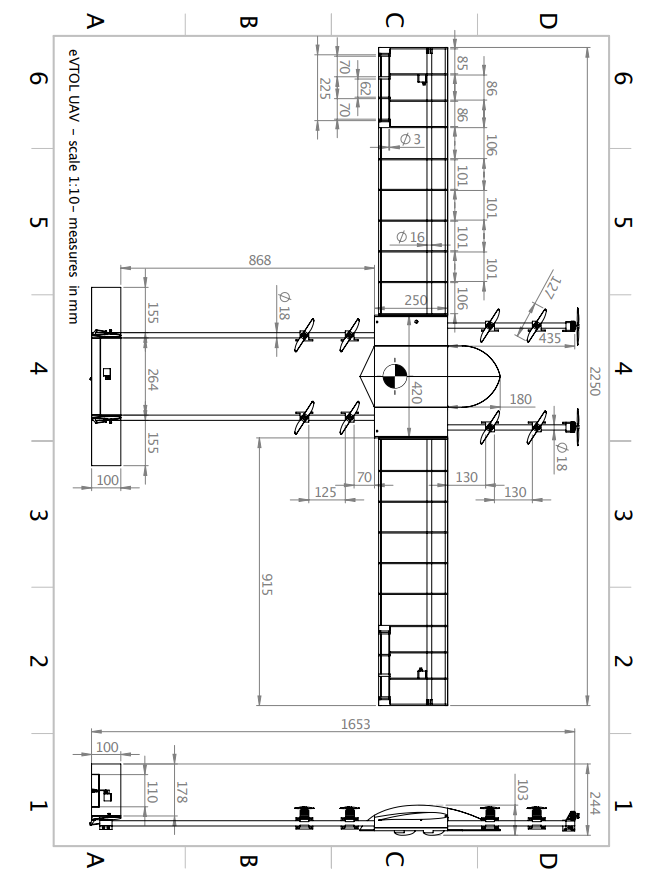
\includegraphics[width=1\linewidth]{Images/Technical drawings of the eVTOL UAV.png}
    \caption{Technical drawings of the eVTOL UAV, scale 1:10. The measurements are given in mm.}
    \label{fig:Technical drawings}
\end{figure}

\begin{figure}
    \centering
    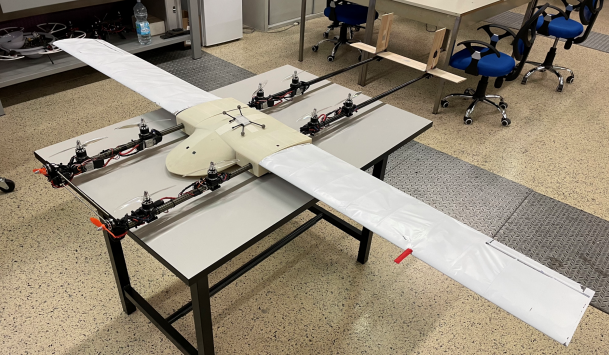
\includegraphics[width=0.75\linewidth]{Images/eVTOL UAV.png}
    \caption{eVTOL UAV developed at P olitecnico di Milano from \cite{battaini2022}}
    \label{fig:eVTOL UAV}
\end{figure}

\section*{Thesis Objectives}

This thesis aims to achieve the following objectives:

\begin{enumerate}
    \item To develop an advanced airframe model of an eVTOL aircraft using MBDyn, a multibody dynamics software, ensuring accuracy and realism in simulating the aircraft's behavior in various flight conditions.
    
    \item To integrate the MBDyn model with Simulink for real-time data exchange and to establish a control system architecture that facilitates precise maneuvering and stability of the eVTOL aircraft.
    
    \item To conduct a comprehensive analysis of the eVTOL aircraft's maneuver performance, particularly focusing on its response and handling qualities in gusty wind conditions as per ADS-33 guidelines.
    
    \item To design and evaluate control strategies for the transition between multi-copter mode and fixed-wing mode in eVTOL aircraft, ensuring smooth and efficient mode switching.
    
    \item To propose a set of quantitative metrics for assessing the agility and maneuverability of eVTOL aircraft, drawing from both UAV-specific and manned aircraft literature.
    
    \item To establish a test procedure and setup for evaluating the maneuvering performance and agility metrics of the eVTOL aircraft through simulations and experimental validations.
    
    \item To identify areas of improvement and provide recommendations for the design and control of eVTOL aircraft, contributing to advancements in the field of aerospace engineering.
\end{enumerate}

These objectives form the foundation of the research and guide the investigation into the capabilities and performance of eVTOL aircraft.

\section*{Structure of the Thesis}

This thesis is meticulously organized to present a cohesive study on the maneuver performance, modeling, and control of an eVTOL aircraft. The structure is as follows:

\begin{itemize}
    \item \textbf{Chapter 1: MBDyn and Airframe Modeling}
    This chapter introduces the fundamental principles of MBDyn, a multibody dynamics software package, and its application in constructing an accurate airframe model. The setup and verification process of the model are discussed in detail.
    
    \item \textbf{Chapter 2: Integration and Control of Subsystems}
    Building upon the airframe model, this chapter outlines the integration process between MBDyn and Simulink. It presents the architecture of the control system, emphasizing the importance of reference frames and rotational principles in aerospace engineering and navigation.
    
    \item \textbf{Chapter 3: Maneuver Performance}
    Chapter 3 evaluates the aircraft's maneuver performance, particularly its response to gust wind conditions as per ADS-33 guidelines. The chapter details the experimental setup, simulation results, and analysis of the aircraft's stability and controllability.
\end{itemize}

\chapter{MBDyn and Airframe Modeling}
\label{ch:chapter1}

This chapter introduces the fundamental principles of MBDyn, a multibody dynamics software package. The key setup of the MBDyn program is discussed, followed by an overview of the relevant MBDyn modules essential for modeling an airframe. Finally, the chapter delves into the specific steps involved in constructing and verifying the accuracy of the airframe model.

\section{MBDyn Software Simulator}
This research utilizes MBDyn, a free multibody dynamics software developed by the Department of Aerospace Engineering (DIAPM) at Politecnico di Milano, Italy. MBDyn offers inherent capabilities for external communication through both local and network configurations. This communication is facilitated by internet and Unix domain sockets, acting as bidirectional communication endpoints at the kernel level. The Stream driver function within MBDyn enables this communication.

Based on the works in \cite{battaini2020}, \cite{martello2021}, and \cite{battaini2022}, the structure of the airframe in \cite{martello2021} was used to build the flight equations of motion with kinematic and dynamic equations in \textit{Simulink} software. Furthermore, a control system was developed for both multi-copter mode and fixed-wing mode. Due to the limitations of the simplified equations of motion, it is challenging to simulate the real conditions of vehicle flight in complex environments. Current airframe modeling schemes may not fully capture the complexities of real-world systems. This necessitates the development of more advanced approaches to achieve more realistic simulations.

MBDyn provides a valuable alternative for simulating the airframe, potentially leading to more realistic results compared to traditional methods \cite{Migliore2019}. This enhanced realism stems from MBDyn's ability to model complex interactions within the airframe. However, the control system design will follow the approach outlined in the references, utilizing \textit{Simulink} for further analysis of drone maneuver performance in subsequent chapters. This choice leverages the extensive analysis tools offered by MATLAB. It is important to note that alternative software could be employed for the control system design to avoid dependence on commercial software.

\subsection{Unconstrained Dynamics}
Because the airframe can move freely in all six degrees of freedom (DoF), the equations governing its motion are described as unconstrained dynamics. We can derive the equations of motion (EOMs) for this unconstrained system using the well-established Newton-Euler approach.

The equations of motion (EOMs) of a general mechanical system are usually derived by the Newton-Euler approach. For a system of unconstrained bodies, EOMs are described by:

\begin{equation}
     M(q) \ddot{q} = l(q, \dot{q}, t)  \label{eq:4_1_1}
\end{equation}

\( l(q, \dot{q}, t) \) is the function describing the external forces acting on nodes and may include structural deformability contributions.

Written in the form of a first-order system, equation \ref{eq:4_1_1} becomes:

\begin{equation}
    M(q) \dot{q} = p \label{eq:4_1_2a}
\end{equation}
\begin{equation}
    \dot{p} = l(q, \dot{q}, p, t) \label{eq:4_1_2b}
\end{equation}

where \( p \in \mathbb{R}^n \) is the momenta and momentum moments vector.

\subsection{Constrained Dynamics}

There exist two types of constraints, holonomic and non-holonomic. Both are modeled by adding explicit algebraic relations:

\textbf{Holonomic Constraints:}
\begin{equation}
    0 = \Phi(q, t) \label{eq:4.1.3}
\end{equation}

\textbf{Non-holonomic Constraints:}
\begin{equation}
    0 = \Psi(q, \dot{q}, t)) \label{eq:4.1.4}
\end{equation}

By using Lagrange’s multipliers formalism, system \ref{eq:4_1_2b} becomes:
\begin{equation}
    M(q) \dot{q} = p ) \label{eq:4.1.5a}
\end{equation}
\begin{equation}
    \dot{p} + \Phi^T/q\lambda + \Psi^T/\dot{q}\mu = l(q, \dot{q}, p, t) \label{eq:4.1.5b}
\end{equation}
\begin{equation}
    \Phi(q, t) = 0 \label{eq:4.1.5c}
\end{equation}
\begin{equation}
    \Psi(q, \dot{q}, t) = 0 \label{eq:4.1.5d}
\end{equation}

where \( \lambda \) and \( \mu \) are the Lagrange’s multipliers.

\section{Numerical Integration}
MBDyn's analyses are based on a unique formulation for the direct time integration of initial value problems (IVPs). These IVPs are expressed as a system of first-order differential-algebraic equations (DAEs) and are solved using implicit, nearly L-stable integration algorithms.

Numerical integration is a fundamental computational technique used to approximate solutions for ordinary differential equations (ODEs) or DAEs. In systems where analytical solutions are impractical, numerical integration plays a crucial role in simulating dynamic behavior across various fields, including engineering and physics.

The Differential Algebraic Equation (DAE) system \ref{eq:4_1_2b} has the general form:

\begin{equation}
    h(\dot{x}, x, t) = 0 \label{eq:4.1.6}
\end{equation}

where \( x = (q, p, \lambda, \mu)^T \).

The numerical solution at time \( t_{k+1} \) using the general multistep method is obtained by solving equation \ref{eq:4.1.6} for \( \dot{x}_{k+1} \) with:

\begin{equation}
    x_{k+1} = \sum_{j=0}^{p-1} (a_j x_{k-j} + h b_j \dot{x}_{k-j}) + h b_p \dot{x}_{k+1} \label{eq:4.1.7}
\end{equation}

Using a Newton-Raphson scheme, the solution is given by:

\begin{equation}
    h_{/\dot{x}} \delta \dot{x}_{k+1} + h_{/ x} \delta x_{k+1} = -h  \label{eq:4.1.8}
\end{equation}

Inserting equation \ref{eq:4.1.7} into equation \ref{eq:4.1.8} yields:

\begin{equation}
    \left(h_{/ \dot{x}} + h b_p h_{/ x}\right) \delta \dot{x}_{k+1} = -h \label{eq:4.1.9}
\end{equation}

because:

\begin{equation}
    \delta x_{k+1} = h b_p \delta \dot{x}_{k+1} \label{eq:4.1.10}
\end{equation}

For each time step (that is, for each instant \( t_k \) of the time grid), iterations are performed to solve equation \ref{eq:4.1.9} until convergence is reached.

\subsection{Two-Step BDF Method}
The Two-Step BDF method is a specific variant of the Backward Differentiation Formula (BDF) family, designed for solving stiff ODEs and DAEs. Unlike explicit methods, which rely solely on information from the current time step, the Two-Step BDF method utilizes data from two preceding time steps to enhance stability and accuracy. This property makes it particularly suitable for systems with widely varying dynamics' time scales, where explicit methods struggle to maintain stability.

The formulation of the Two-Step BDF involves constructing polynomial approximations to the solution using backward differences. Let \( y_n \) denote the solution at time \( t_n \) and \( \Delta t \) denote the time step size. The backward difference approximation for the derivative \( y'(t_n) \) is given by:

\begin{equation}
    y'(t_n) \approx \frac{1}{\Delta t} \left( \alpha_0 y_n + \alpha_1 y_{n-1} + \alpha_2 y_{n-2} \right)
\end{equation}

where \( \alpha_0 \), \( \alpha_1 \), and \( \alpha_2 \) are coefficients determined by the Two-Step BDF method. By incorporating these approximations into the differential equations, the Two-Step BDF method yields implicit equations that are solved iteratively at each time step, often using techniques like Newton's method.

The Two-Step BDF method offers several advantages over other numerical integration techniques. Firstly, it exhibits stability and efficiency, especially in handling stiff systems characterized by both fast and slow dynamics. Unlike explicit methods, which require excessively small time steps to maintain stability in stiff systems, the Two-Step BDF method allows for larger time steps while preserving stability, leading to significant computational savings.

Additionally, the Two-Step BDF method offers second-order accuracy, contributing to more precise solutions, particularly over longer integration intervals, compared to lower-order methods.

\subsection{Block Scheme Simulator}

This kind of simulators have been developed for many years by different groups: examples are \textit{Simulink} \cite{Simulink} by Mathworks, SystemBuild \cite{SystemBuild} by National Instruments, and the Scicos \cite{Scicos} based ScicosLab \cite{ScicosLab} by INRIA and Xcos \cite{Xcos} by the Scilab Consortium.

Considering the efficiency and the versatility, \textit{Simulink} is probably the best simulator available. On the other side, if the user freedom related to the software is the argument driving the comparison, ScicosLab becomes the best candidate. All the indicated simulators, though, are widely recognized by the industry and the academic world to be valid instruments.

\subsection{Inter-process Communication}

The inter-process communication is constructed based on TCP/IP Internet sockets (with the local communication being a special subcase of the network-based data exchange). This kind of data transmission is very efficient (way more than, for example, employing text file read/write functions), and it is naturally directed to multiple machines layout, which, in many cases, can sensitively decrease the time-to-solution.

\section{Airframe Modeling}
The structure of an eVTOL aircraft is designed to enable vertical takeoff and landing, as well as efficient horizontal flight. It typically includes a frame for support, propulsion systems with 8 vertical propellers and 2 horizontal propellers, wings with main wing, horizontal and vertical tail wings, a fuselage including onboard batteries for power, and space for sensors.

\begin{figure}[h]
    \centering
    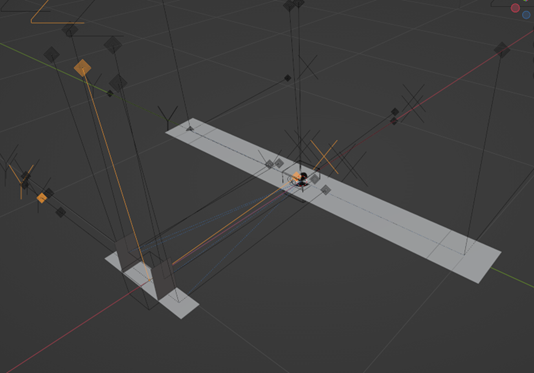
\includegraphics[width=0.9\linewidth]{Images/MBDyn model in blender.png}
    \caption{MBDyn model in Blender.}
    \label{fig:MBDyn_model_in_blender}
\end{figure}

\subsection{Reference System}
A reference system can be seen as a coordinate system used to describe the positions and orientations of elements. Because reference systems can be recursively built on each other, the process of building or transforming an MBDyn model is much easier when utilizing a reference system rather than building a model in the global system.

\subsection{Constitutive Law}
\label{section:Constitutive_law}
To realize the effect of ground contact, a Constitutive Law Module is applied in MBDyn, providing various formulas for 1D continuous contact models. This module can also function as a 3D constitutive law, under the assumption that the 1D formulas are applied with respect to the third direction of the associated 3D entity. In this case, the component three of strain and strain rate are utilized as inputs, and the output force is applied along direction three.

The Constitutive Law Module supports multiple models, including Flores, Hunt-Crossley, and Lankarani-Nikravesh. For this MBDyn model, the Flores model is used as the default. The dissipation coefficient (\(\text{dissipation\_coef}\)) is determined by the equation:

\begin{equation}
    \text{dissipation\_coef} = \frac{8}{5} \cdot \text{stiffness} \cdot \frac{1 - \text{restitution\_coef}}{\text{restitution\_coef} \cdot \dot{x}_0}
\end{equation}

It's important to note that the restitution coefficient (\(\text{restitution\_coef}\)) must satisfy \(0 < \text{restitution\_coef} \leq 1\). The stiffness parameter can be adjusted to approximate the behavior of the real ground. However, choosing an excessively high stiffness may cause the MBDyn simulation to stop abruptly if the drone experiences a hard impact with the ground. Therefore, a reasonable coefficient should be selected, balancing realism with stability.

A specific set of parameters for the constitutive law is chosen, as outlined in Table \ref{tab:Constitutive_law}.

\begin{table}[h]
    \centering
    \begin{tabular}{ccc}
    \hline
    Restitution Coefficient & Stiffness (\(\kappa\)) & Exponential Term \\
    \hline
    0.8 & \(2.4 \times 10^3\) & 1.5 \\
    \hline
    \end{tabular}
    \caption{Constitutive Law configuration}
    \label{tab:Constitutive_law}
\end{table}

To implement the constitutive law, 1 static node needs to be used to clamp on the ground, and 4 deformation displacement joints need to be used in 4 directions. A rigid free fall body from 1 meter height (figure \ref{fig:freefall}) is employed to evaluate the ground effect using the Constitutive Law Module.

\begin{figure}
    \centering
    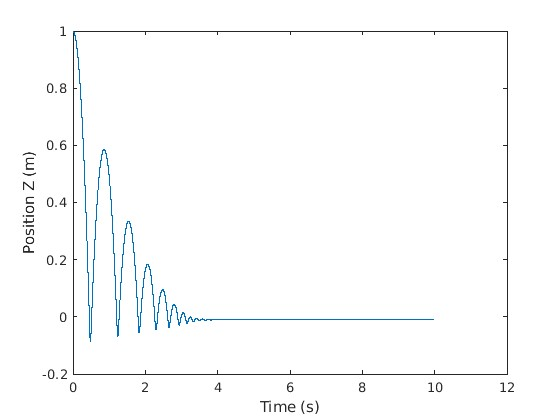
\includegraphics[width=0.5\linewidth]{Images/freefall.jpg}
    \caption{Position Change in Z-axis of free fall simulation.}
    \label{fig:freefall}
\end{figure}

\subsection{Data} 
The data module serves as the input mechanism, defining the geometry, physical properties, and initial conditions of the model.

\subsection{Initial Value} 
This module specifies the starting state of the model, including initial positions, velocities, and other parameters necessary for simulation initialization. The setup in the simulator is shown below.
\begin{itemize}
    \item Initial time: \(0\)
    \item Final time: \(100\)
    \item Time step: \(10^{-3}\)
    \item Tolerance: \(1 \times 10^{-10}\)
    \item Max iterations: \(10\)
    \item Derivatives tolerance: \(10\)
    \item Derivatives max iterations: \(200\)
    \item Derivatives coefficient: \(1 \times 10^{-3}\)
    \item Method: BDF
\end{itemize}

\subsection{Control Data} 
Control Data enables users to specify fundamental simulation parameters, including duration, time step size, and other global settings essential for the progression of the simulation process.

\textbf{Solver Configuration:} MBDyn offers a variety of solvers for simulating mechanical systems. Within the control data section, users can designate the preferred solver and configure its parameters, such as integration methods, convergence criteria, and tolerances.

\textbf{Output Configuration:} Users can define the desired output data, encompassing motion trajectories, forces, accelerations, and other pertinent information crucial for analysis and visualization purposes.

\textbf{Control Strategy:} Dynamic systems often require sophisticated control strategies to regulate system behavior over time. The control data section empowers users to define control algorithms, such as PID controllers or custom strategies, facilitating precise management of system dynamics during simulation.

\textbf{Error Handling and Logging:} MBDyn offers robust error handling and logging mechanisms during simulations. Users can specify error handling procedures and logging configurations to facilitate diagnosis and troubleshooting of simulation issues effectively.
\begin{verbatim}
begin: control data;
    structural nodes:
        +1      # CLAMP
        +1      # Mass Center
        +1      # ground
        +10     # dummy
    ;
    rigid bodies:
        1       # main body
    ;
    joints:
        +1      # ground clamp
        +1      # Mass Center
        +4      # constitutive law
    ;
    forces:
        20      # thrust and torque of propllers
    ;
    aerodynamic elements:
        +3      # Main
        +3      # H Tail
        +2      # V Tail
        +11     # aircraft intrument
    ;
    abstract nodes:
        +10     # angular velocity of motor
        +3      # Movable Surface
    ;
    genels:
        +10     # angular velocity delay function of motor
        +3      # Movable Surface
    ;
    gravity;
    air properties;
    output results : netcdf;
    output elements: 1;
    file drivers: 1;
    default orientation: euler321;
    default output: all;
end: control data;
\end{verbatim}

\subsection{Nodes} 
Nodes represent connection points or joints within the model, facilitating interactions between different components and defining the model's motion.

The type of nodes in MBDyn can be one of the following categories:
\begin{itemize}
    \item abstract
    \item electric
    \item hydraulic
    \item parameter
    \item structural
    \item thermal
\end{itemize}

\subsubsection{Structural Node}
Structural nodes can possess either six degrees of freedom (DOF), representing both position and orientation and thus describing the kinematics of rigid-body motion in space, or three degrees of freedom, representing position only and describing the kinematics of point mass motion in space.

The six-DOF structural node can be categorized as static, dynamic, modal, or dummy, while the three-DOF structural node can be either static or dynamic. Elements requiring only displacement can be connected to either type of node; however, when connected to a six-DOF node, they utilize solely position and velocity, contributing solely to force equilibrium equations. Elements necessitating both displacement and orientation are exclusive to six-DOF nodes.

\textbf{Static Node:} The static keyword means no inertia is related to that node, so it must be appropriately constrained or attached to elastic elements. Static nodes are useful when there is no need to apply inertia to them, thus saving 6 degrees of freedom. In this airframe, 1 static node (\textit{ClampNode}) is applied which is introduced in section \ref{section:Constitutive_law}.

\textbf{Dynamic Node:} The dynamic keyword means inertia can be attached to the node, so it provides linear and angular momenta degrees of freedom and automatically generates the so-called automatic structural elements. 2 Dynamic nodes (\textit{MassCenter}, \textit{ROOT}) need to be used, \textit{MassCenter} is a center to be acted on by aerodynamic force and propeller force and torque. \textit{MassCenter} and \textit{ROOT} are connected with 1 total joint to represent the force and torque which could be monitored in other software.

\textbf{Dummy Node:} The dummy structural node serves the purpose of facilitating the visualization of the kinematics of arbitrary points within the system during simulation. Unlike other structural nodes, the dummy node does not introduce any degrees of freedom itself; rather, it must be connected to another node within the system. This feature enhances the comprehensibility of the simulation output by allowing users to track the motion and behavior of specific points within the system. 10 dummy nodes are used in this airframe in each position of the propeller to apply the aircraft instruments which are introduced in section \ref{section:Aerodynamic elements}.

\subsubsection{Abstract Node}
Abstract nodes are ancestors of all scalar node types. Many general and electric elements can be connected to abstract nodes as well, since they directly use the ancestor class. 10 abstract nodes (\textit{ForceV1-8}, \textit{ForceH1}, \textit{ForceH2}) are used to apply the time delay and obtain the angular velocity of each propeller.

\subsection{Drivers} 
External forces or inputs applied to the model are defined by the drivers module, allowing users to simulate real-world effects and interactions.

\subsubsection{File Drives}
The \textit{Simulink} control system employs a WebSocket module to establish a connection with the MBDyn model. The input command comprises 12 inputs: the first three inputs control the surfaces for the aileron, elevator, and rudder respectively. Inputs 4 to 11 control the throttle for each vertical propeller, while 12 and 13 input controls the throttle for two horizontal propellers.

\subsection{Elements} 
Elements encompass the physical components or bodies within the model, defining their geometry, material properties, and connectivity.

\subsubsection{Rigid Body Element} 
The body element offers the possibility to add a point mass to a structural node. Additionally, inertia can be set.

In consideration of simulation accuracy and computation cost, the main structure in MBDyn is simplified to include only rigid bodies, due to the complex physical shape and negligible aerodynamic effect. The fuselage and the connecting components are neglected. To upgrade the structure of the airframe and provide the relevant information, including mass and inertia moment, the new values are as follows:

\begin{itemize}
    \item Mass: 6.4 kg
    \item Inertia Moment:
    \[
    \begin{pmatrix}
    0.3724 & 0.0004 & 0.0083 \\
    0.0004 & 0.7237 & 0 \\
    0.0083 & 0 & 1.0868 \\
    \end{pmatrix}
    \]
\end{itemize}

With these updated values, the airframe's mass and inertia moment are now accurately represented within the simulation environment. This enhanced structural representation ensures improved fidelity in the simulation results while balancing computational efficiency.

\subsubsection{Joint Element}
Since nodes must be constrained properly to satisfy the equilibrium equations in MBDyn, the joint element can be used to satisfy this request. Additionally, joints can be used to connect nodes together, relatively constraining certain degrees of freedom.

\textbf{Clamp Joint:} The clamp joint element constrains a node at all 6 degrees of freedom. Thus, this element can ideally be used to fix a base node, from which all other elements depend.

\textbf{Total Joint:} With the total joint element, constraints in each degree of freedom can be defined separately. Hereby MBDyn distinguishes between position and orientation constraints. Additionally, the constraints can be influenced in its value using a drive caller. Overall, this element can be used to arbitrarily define nodes' positions and motions.

\textbf{Deformable Displacement Joint:} This joint implements a configuration-dependent force that is exchanged between two points associated with two nodes with an offset. The force may depend, by way of a generic 3D constitutive law, on the relative position and velocity of the two points, expressed in the reference frame of node 1. The constitutive law is attached to the reference frame of node 1, so the sequence of the connections may matter in case of anisotropic constitutive laws if the relative orientation of the two nodes changes during the analysis.

\subsubsection{Force Element}
\label{section:force elements}
The force element has two types of forces that could be applied: structural and abstract. Structural forces have three components that may depend on arbitrary parameters (usually the simulated time) and a location in space. Structural couples have three parameter-dependent components.

Considering the difficulty and high computation cost of building each propeller with actual elements, currently, propeller parts are simplified as structural forces and torques applied at corresponding positions. The \textit{follower} in force and torque keeps the direction of force and moment fixed with the attitude of the main body of the airframe. The propulsion system consists of 8 propellers in the vertical direction, 4 of them are in front of the main wing, and another 4 vertical propellers are on the back of the main, and 2 horizontal propellers which are at the nose of the airframe. The actual positions are shown in Figure \ref{fig:Aircraft top view}.

\begin{figure}
    \centering
    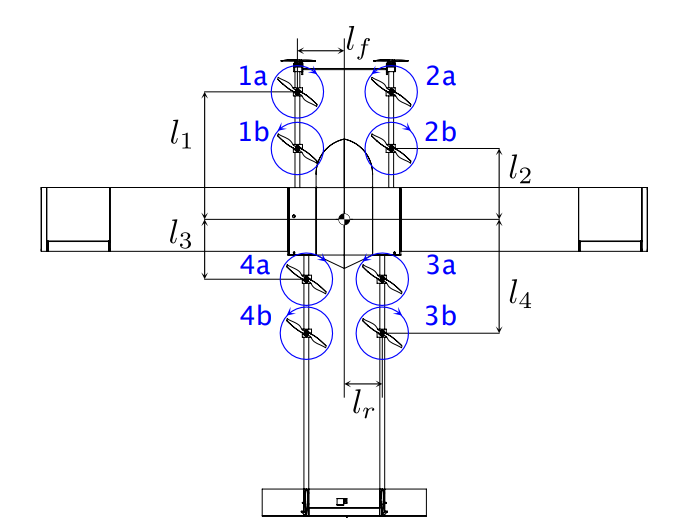
\includegraphics[width=0.8\linewidth]{Images/Aircraft top view.png}
    \caption{Aircraft top view, with relevant dimensions named, propellers numbering and propellers spinning directions.}
    \label{fig:Aircraft top view}
\end{figure}

The control system sends throttle command to rotor motors which drive vertical and horizontal propellers to achieve designed angular velocity to generate thrust and torque to provide the drone with lift and moments. The vertical propeller is controlled in multi-copter mode, and the horizontal propeller is controlled in fixed-wing mode. Considering the high computation cost of building each propeller with detailed aerodynamic bodies, the rotor is simplified as forces and moments at each rotor position.

In \cite{battaini2022}, Each of the propellers exerts a thrust and torque proportional to the square of the angular velocity:

\begin{equation}
    T_i = K_T \Omega_i^2,  K_T = C_T \rho A R^2, \label{eq:thrust} 
\end{equation}
\begin{equation}
    Q_i = K_Q \Omega_i^2,  K_Q = C_Q \rho A R^3, \label{eq:torque}
\end{equation}
where $C_T$ and $C_Q$ are the thrust and torque coefficients, $\rho$ is the air density, $A$ and $R$ are respectively the area of the propeller disk and its radius, and $\Omega_i$ is the rotational speed of the $i$-th propeller.

Previous work in \cite{battaini2022} simplified the propeller without considering the incoming flow, leading to high errors in real-world situations when the drone climbs, descends in multi-copter mode, or moves forward at high speed in fixed-wing mode. This section aims to optimize these equations. To consider the influence of inflow air, blade momentum theory and blade element theory need to be used.

\textbf{Blade Momentum Theory}

Blade Momentum Theory is a simplified method used to analyze the aerodynamic performance of rotor blades in rotary-wing aircraft such as helicopters \cite{Leishman2006}. It is based on the principle of conservation of momentum and assumes that the rotor extracts a constant amount of momentum from the air per unit time. The basic equation governing Blade Momentum Theory is:
\begin{equation}
    T = \dot{m} \cdot \Delta v \label{eq:Blade Momentum Theory}
\end{equation}
where:
\begin{itemize}
    \item $T$: Thrust produced by the rotor.
    \item $\dot{m}$: Mass flow rate of air through the rotor.
    \item $\Delta v$: Change in air velocity across the rotor.
\end{itemize}
The mass flow rate $\dot{m}$ is given by:
\begin{equation}
    \dot{m} = \rho \cdot A \cdot V
\end{equation}
where:
\begin{itemize}
    \item $\rho$: Air density.
    \item $A$: Rotor disk area.
    \item $V$: Airspeed.
\end{itemize}

\textbf{Blade Element Theory}

The blade element approach for the analysis of helicopter rotors has been well established \cite{Leishman2006}. The resultant local flow velocity at any blade element at a radial distance $y$ from the rotational axis has an out-of-plane component $U_P=V_c+v_i$ normal to the rotor as a result of climb and induced inflow and an in-plane component $U_T=\Omega y$ parallel to the rotor because of blade rotation, relative to the disk plane. The resultant velocity at the blade element is, therefore,
\begin{equation}
U=\sqrt{U_T^{2}+U_P^{2}}.
\end{equation}
The relative inflow angle (or induced angle of attack) at the blade element will be
\begin{equation}
\phi=\tan^{-1}\left(\frac{U_P}{U_T}\right)\approx\frac{U_P}{U_T} \text{ for small angles.}
\end{equation}
Thus, if the pitch angle at the blade element is $\theta$, then the aerodynamic or effective angle of attack is
\begin{equation}
\alpha=\theta-\phi=\theta-\frac{U_P}{U_T}.
\end{equation}
The resultant incremental lift $dL$ and drag $dD$ per unit span on this blade element are given by:
\begin{equation}
dL=\frac{1}{2}\rho U^{2}cC_l dy
\end{equation}
and
\begin{equation}
dD=\frac{1}{2}\rho U^{2}cC_d dy,
\end{equation}
where $C_l$ and $C_d$ are the lift and drag coefficients, respectively, and $c$ is the local blade chord.

\textbf{Thrust Approximation:} Based on steady linearized aerodynamics, the local blade lift coefficient can be written as
\begin{equation}
C_l = C_{l\alpha}(\alpha - \alpha_0) = C_{l\alpha}(\theta - \alpha_0 - \varphi),
\end{equation}
where $C_{l\alpha}$ is the 2-D lift-curve-slope of the airfoil section(s) comprising the rotor, and $\alpha_0$ is the corresponding zero-lift angle. For an incompressible flow, $C_{l\alpha}$ would have a value close to the thin-airfoil result of $2\pi$ per radian. Also, unless otherwise stated, it will be assumed that $\alpha_0$ can be combined into $\theta$.

Therefore, $C_{L_{w}}$ can be taken outside of the integral sign giving
\begin{equation}
    C_{T}=\frac{1}{2}\sigma\int_{0}^{1}C_{l}r^{2}dr=\frac{1}{2}\sigma~C_{l_{a}}\int_{0}^{1}(\theta-\phi)r^{2}dr,
\end{equation}
and using the result that $\phi=\lambda/r$ then the thrust coefficient can be written as
\begin{equation}
    C_{T}=\frac{1}{2}\sigma~C_{k}\int_{0}^{1}(\theta r^{2}-\lambda r)dr.
\end{equation}
In the condition of Untwisted Blades in Uniform Inflow, for a blade with zero twist, $\theta$ is constant ($\theta_0$), and for uniform inflow velocity, which is assumed in simple momentum theory, $\lambda$ is constant. Therefore, in this case, the thrust coefficient is given by
\begin{equation}
    C_{T}=\frac{1}{2}\sigma~C_{l_{*}}\int_{0}^{1}(\theta_{0}r^{2}-\lambda r)dr=\frac{1}{2}\sigma~C_{l_{*}}\left[\frac{\theta_{0}r^{3}}{3}-\frac{\lambda r^{2}}{2}\right]_{0}^{1}=\frac{1}{2}\sigma~C_{l_{a}}\left[\frac{\theta_{0}}{3}-\frac{\lambda}{2}\right]
\end{equation}

\textbf{Optimized derived Thrust and Torque of Rotor}

Based on these assumptions, (\ref{eq:Blade Momentum Theory}) from Blade Momentum Theory could be written as:
\begin{equation}
    T = 2 \rho A (v_c + u) u \label{eq:thrust_1}
\end{equation}
where:
\begin{itemize}
    \item $u$: outcome airflow.
    \item $v_c$: income airflow.
\end{itemize}
And in Blade Element Theory:
\begin{equation}
    \lambda = \frac{{(v_c + u)}}{{\omega R}}    \label{eq:thrust_2}
\end{equation}
\begin{equation}
    C_T = \frac{1}{2} \sigma C_{L\alpha} B^2 \left( \frac{{\theta B}}{3} - \lambda \right)  \label{eq:thrust_3}
\end{equation}
the thrust of the propeller could be written as:
\begin{equation}
    F = C_T \rho A \omega^2 R^2 \label{eq:thrust_4}
\end{equation}
Combining (\ref{eq:thrust_1}), (\ref{eq:thrust_2}), (\ref{eq:thrust_3}), and (\ref{eq:thrust_4}), the induced velocity in a generic cross-section is obtained:
\begin{equation}
    u = \sqrt{\frac{{B^4 C_{L\alpha}^2 \omega^2 R^2}}{{16}} + \frac{{4 \theta B^3 C_{L\alpha} \omega^2 R^2}}{3} - B^2 C_{L\alpha} \omega R v_c + 4 v_c^2} / 4 - \frac{{v_c}}{2} - \frac{{B^2 C_{L\alpha} \omega R}}{16}  \label{eq:outcome_airflow}
\end{equation}
(\ref{eq:outcome_airflow}) deviates the outcome airflow with the income airflow correction. Based on this, the corrected rotor thrust coefficient could be obtained by (\ref{eq:thrust_3}). For the torque generated by the propeller, in Torque-power approximations, according to blade element theory, by assuming uniform inflow and $C_d = C_{d0} = \text{constant}$, the torque coefficient with the inflow air correction could be obtained as:
\begin{equation}
    C_Q = \lambda C_T + \frac{1}{8} \sigma C_{d0}
\end{equation}
\cite{battaini2022} upgraded the motor and vertical propellers. After optimization, the new propellers used in the airframe are:

According to the propeller dimensions and experimental data provided in \cite{battaini2022}, the data used in the propeller is summarized in Table \ref{tab:propeller_specs}.

\begin{table}[h]
\centering
\caption{Propeller Coefficients}
\label{tab:propeller_specs}
\begin{tabular}{@{}lllllll@{}}
\hline
Propeller Type & Format & Dimension & $B$ & $\theta_0$ & $\sigma$ & $C_{D\alpha}$ \\
\hline
Horizontal & KDE 2304XF-2350 & 5x4.5 inch & 0.98 & $13^\circ$ & 0.187 & 0.26 \\
Vertical & KDE 2315XF-2050 & 7x4.2 inch & 0.98 & $17.3^\circ$ & 0.122 & 0.85 \\
\hline
\end{tabular}
\end{table}

\textbf{Comparison with MBDyn Rotor Model}

To prove the accuracy of derived thrust and torque equations, the previous thrust and moment equations applied in \cite{battaini2022} are also computed, and a detailed rotor aerodynamic MBDyn model is used as a reference to compare the thrust and torque in the same work condition. The data obtained in the previous section are used to build the MBDyn rotor model:

\begin{itemize}
    \item BLADE\_TWIST = 0
    \item INPUT\_THETA\_0
    \item OMEGA\_100 = 1917
    \item SIGMA
    \item R
    \item N\_B = 2
    \item N\_REVS = 20
\end{itemize}

A typical simulation result of the rotor MBDyn model is shown in Figure \ref{fig:aero_rotor Mbdyn}. After activation of the propeller at the initial phase, the force and moment of the rotor become stable values. The values of force and moment are chosen as the average value in the end phase.

As Figures \ref{fig:aero_rotor Thottle V} and \ref{fig:aero_rotor Thottle H} show, when propellers work without the influence of inflow wind, the force and moment in the optimized equation and MBDyn simulation are basically fit to the old simplified equation computed value. Because the MBDyn model could not build an absolute same model with the real propeller, the value of MBDyn simulation is a little different from the derived optimized equation and simplified equation.

In the simulation condition that constant 100\% throttle command with different inflow wind velocities (Figures \ref{fig:aero_rotor Wind H}, \ref{fig:aero_rotor Wind V}), it could be seen that the force and moment decrease with inflow velocity increase. Due to the MBDyn model accuracy, limitation of optimized equation that neglects the twist angle and tip loss effect, the difference between MBDyn simulation and estimate equation computed value increases with the increase of inflow velocity. Compared with other cases, the moment in the horizontal propeller has high error, but in actual simulation, the rotation orientation is opposite so that the moment value could be neglected. Basically, the optimized equation is enough to apply in actual MBDyn simulation.

The values are summarized in Tables \ref{tab:aero_rotor throttle H}, \ref{tab:aero_rotor throttle V}, and  \ref{tab:aero_rotor wind}.

\begin{figure}
    \centering
    \subfigure[Force]{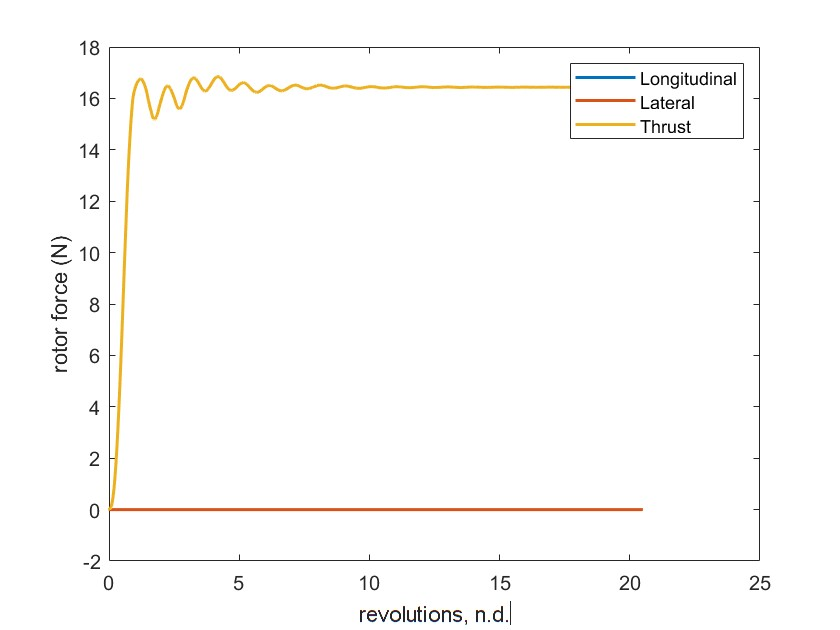
\includegraphics[width=0.3\textwidth]{Images/aero_rotor/aerorotor force_V0.jpg}}
    \hfil % Add some horizontal space between the figures
    \subfigure[Moment]{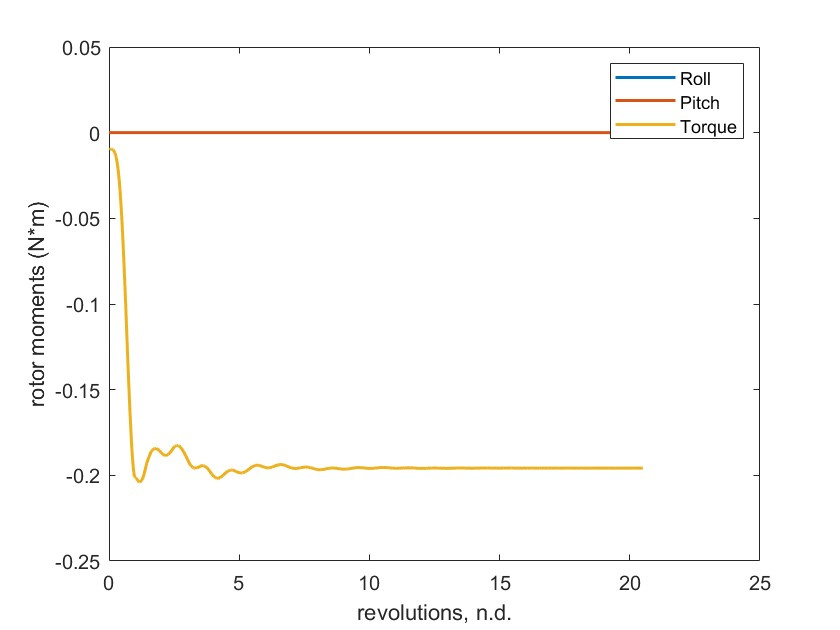
\includegraphics[width=0.3\textwidth]{Images/aero_rotor/aerorotor moment_V0.jpg}}    
    \hfil % Add some horizontal space between the figures
    \subfigure[Induced Velocity]{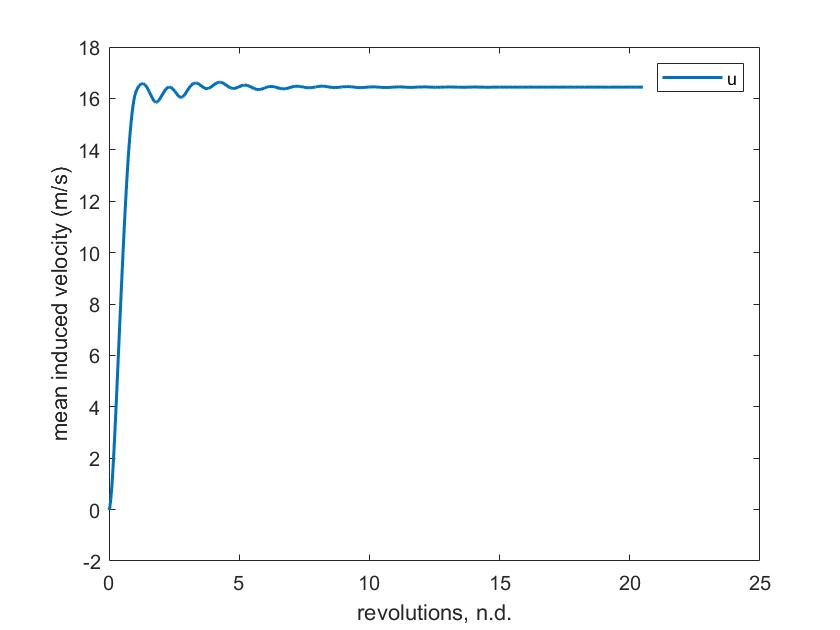
\includegraphics[width=0.3\textwidth]{Images/aero_rotor/aerorotor Velocity_V0.jpg}}    
    \caption{Force and moment change of rotor MBDyn simulation}
    \label{fig:aero_rotor Mbdyn}
\end{figure}

\begin{figure}
    \centering
    \subfigure[Force]{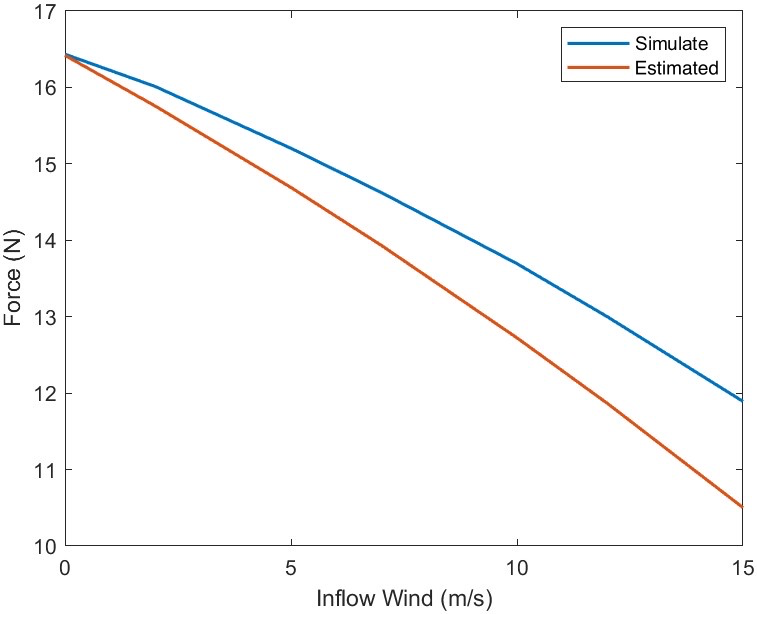
\includegraphics[width=0.4\textwidth]{Images/aero_rotor/aerorotor Force V Wind.png}}
    \hfil % Add some horizontal space between the figures
    \subfigure[Moment]{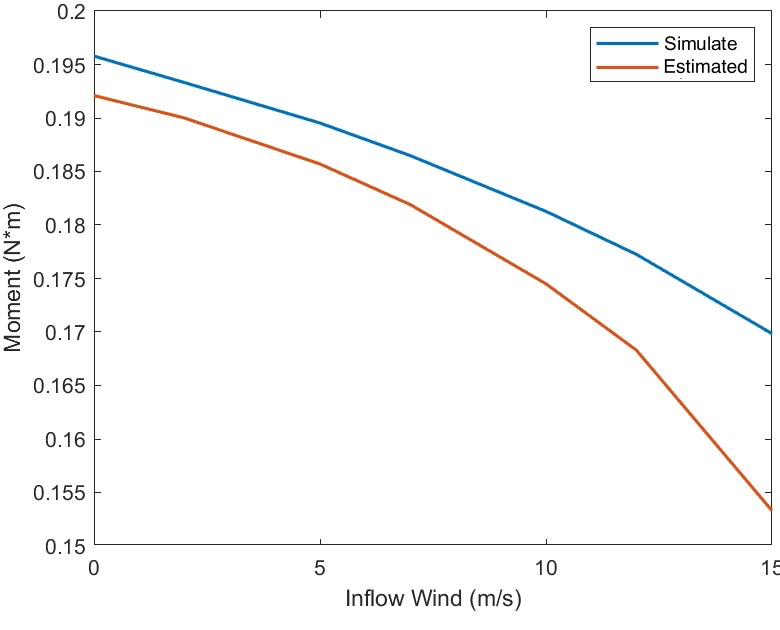
\includegraphics[width=0.4\textwidth]{Images/aero_rotor/aerorotor Moment V Wind.png}}
    \caption{Comparison between optimized equation computed value and MBDyn simulation with change of inflow velocity in vertical propellers.}
    \label{fig:aero_rotor Wind V}
\end{figure}

\begin{figure}
    \centering
    \subfigure[Force]{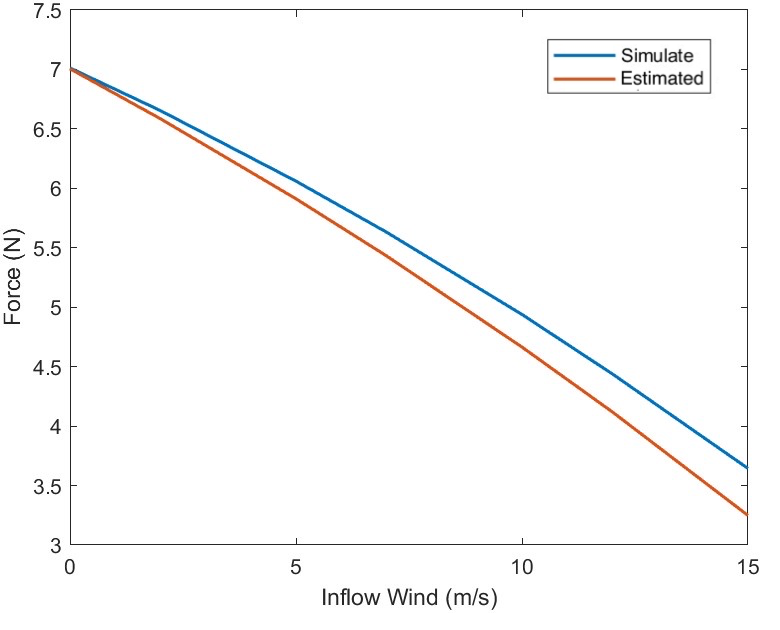
\includegraphics[width=0.4\textwidth]{Images/aero_rotor/aerorotor Force H Wind.png}}
    \hfil % Add some horizontal space between the figures
    \subfigure[Moment]{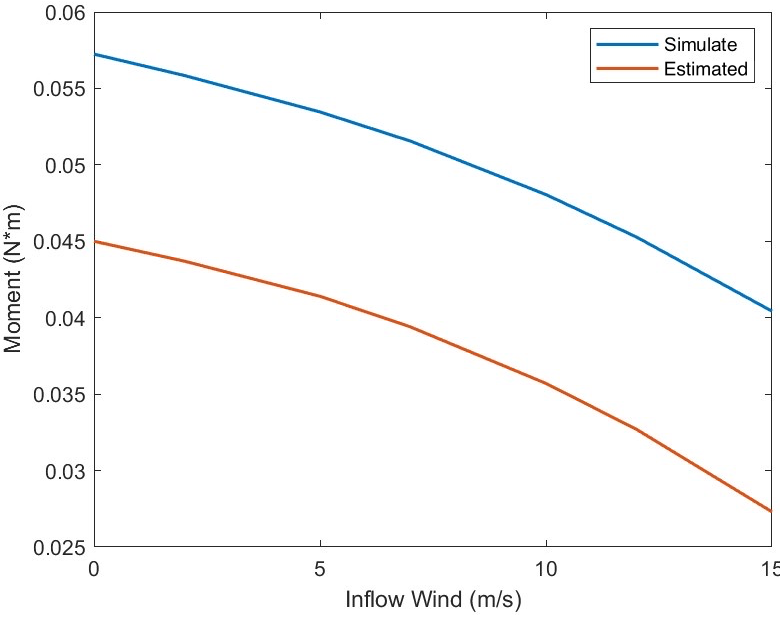
\includegraphics[width=0.4\textwidth]{Images/aero_rotor/aerorotor Moment H Wind.png}} 
    \caption{Comparison between optimized equation computed value and MBDyn simulation with change of inflow velocity in horizontal propellers.}
    \label{fig:aero_rotor Wind H}
\end{figure}

\begin{figure}
    \centering
    \subfigure[Force]{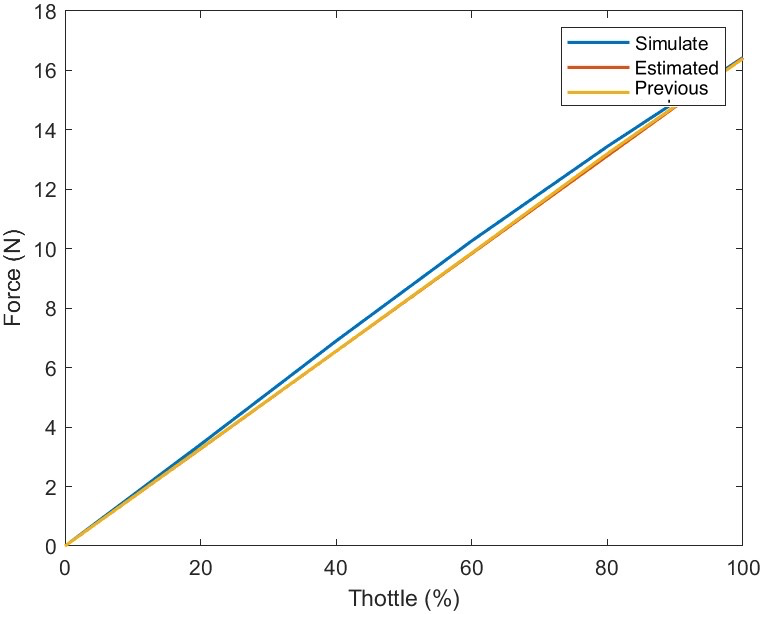
\includegraphics[width=0.4\textwidth]{Images/aero_rotor/aerorotor Force V Thottle.png}}
    \hfil % Add some horizontal space between the figures
    \subfigure[Moment]{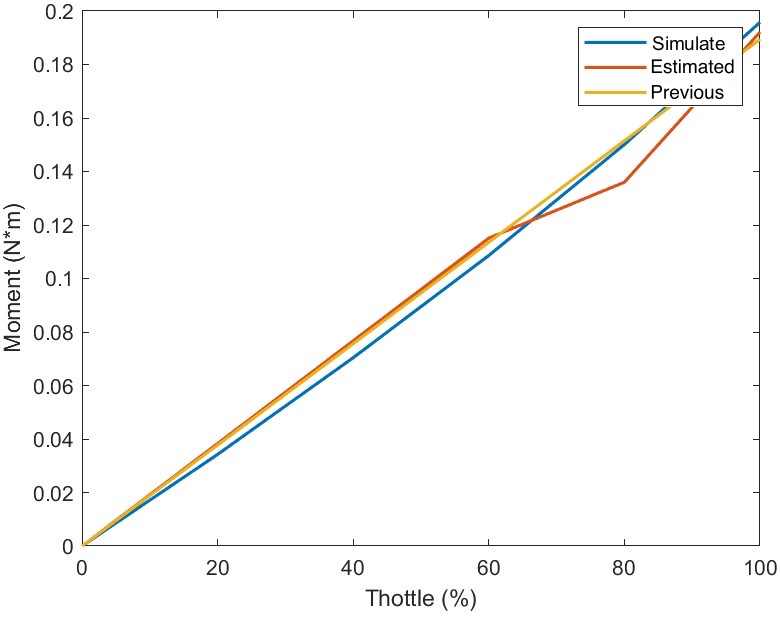
\includegraphics[width=0.4\textwidth]{Images/aero_rotor/aerorotor Moment V Thottle.png}}    
    \caption{Change with Thottle}
    \label{fig:aero_rotor Thottle V}
\end{figure}

\begin{figure}
    \centering
    \subfigure[Force]{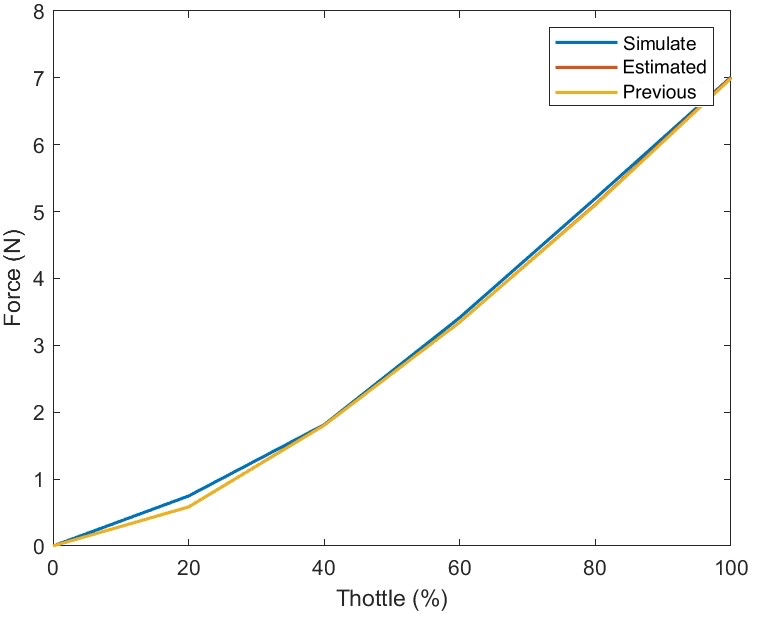
\includegraphics[width=0.4\textwidth]{Images/aero_rotor/aerorotor Force H Thottle.png}}
    \hfil % Add some horizontal space between the figures
    \subfigure[Moment]{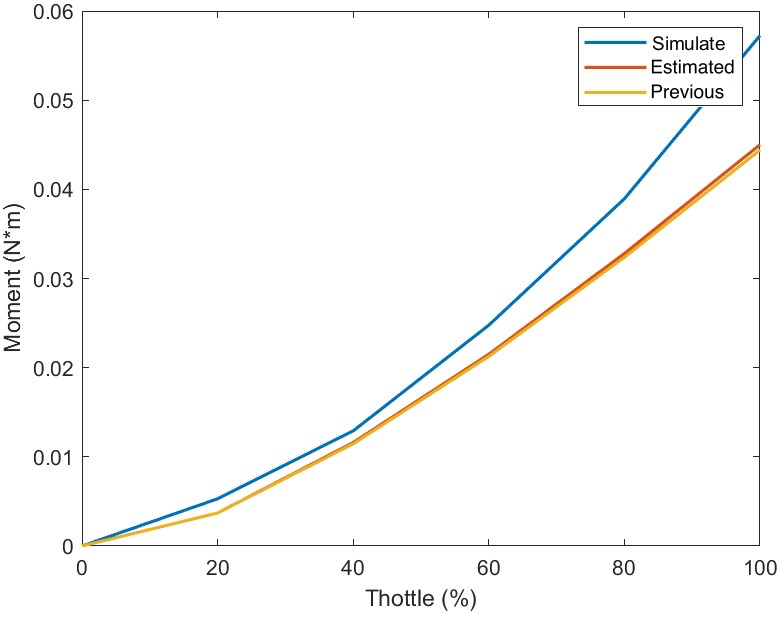
\includegraphics[width=0.4\textwidth]{Images/aero_rotor/aerorotor Moment H Thottle.png}}    
    \caption{Comparison between optimized equation computed value, MBDyn simulation and old simplified equation computed value with change of throttle command.}
    \label{fig:aero_rotor Thottle H}
\end{figure}

\begin{sidewaystable}
\centering
\caption{Comparison between optimized equation computed value and MBDyn simulation with change of inflow velocity in vertical and horizontal propellers.}
\begin{tabular}{c|cc|cc|cc|cc}
\hline
Inflow Velocity (m/s) & \multicolumn{4}{c}{Vertical propeller} & \multicolumn{4}{c}{Horizontal propeller} \\
\hline
       & \multicolumn{2}{c}{Force (N)}  & \multicolumn{2}{c}{Moment (N*m)} & \multicolumn{2}{c}{Force (N)}  & \multicolumn{2}{c}{Moment (N*m)}\\
       \hline
       & Simulation & Estimated & Simulation & Estimated & Simulation & Estimated & Simulation & Estimated \\
       \hline
0      & 16.4345 & 16.4191 & 0.195786 & 0.1921 & 7.01236 & 7.0054 & 0.0572453 & 0.045 \\
2      & 16.0111 & 15.7553 & 0.193313 & 0.19   & 6.65378 & 6.5854 & 0.0558456 & 0.0437 \\
5      & 15.2033 & 14.6906 & 0.189529 & 0.1857 & 6.06021 & 5.9119 & 0.0534594 & 0.0414 \\
7      & 14.6242 & 13.9332 & 0.186478 & 0.1819 & 5.6318  & 5.4323 & 0.0515545 & 0.0394 \\
10     & 13.6939 & 12.7228 & 0.18127  & 0.1745 & 4.93898 & 4.6645 & 0.0480527 & 0.0357 \\
12     & 12.9989 & 11.8653 & 0.177255 & 0.1683 & 4.43862 & 4.1191 & 0.0452798 & 0.0327 \\
15     & 11.8917 & 10.5018 & 0.169847 & 0.1533 & 3.64383 & 3.2484 & 0.0404258 & 0.0273 \\
\hline
\label{tab:aero_rotor wind}
\end{tabular}
\end{sidewaystable}

\begin{table}[htbp]
\centering
\caption{Comparison between optimized equation computed value, MBDyn simulation and old simplified equation computed value in vertical propeller with change of throttle command.}

\begin{tabular}{c|ccc|ccc}
\hline
Throttle(\%) & \multicolumn{3}{c}{Force(N)} & \multicolumn{3}{c}{Moment(N*m)} \\
\hline
 & Simulation & Estimated & Previous & Simulation & Estimated & Previous  \\
 \hline
0   & 0        & 0        & 0        & 0         & 0        & 0         \\
20  & 3.41705  & 3.2702   & 3.275202 & 0.0342378 & 0.0383   & 0.037727  \\
40  & 6.89989  & 6.5544   & 6.564398 & 0.0703868 & 0.0767   & 0.075615  \\
60  & 10.267   & 9.8419   & 9.856905 & 0.108608  & 0.1151   & 0.113541  \\
80  & 13.4427  & 13.1302  & 13.150217& 0.150066  & 0.136    & 0.151476  \\
100 & 16.4345  & 16.4191  & 16.444145& 0.195786  & 0.1921   & 0.189418  \\
\hline
\label{tab:aero_rotor throttle V}
\end{tabular}
\end{table}

\begin{table}[htbp]
\centering
\caption{Comparison between optimized equation computed value, MBDyn simulation and old simplified equation computed value in horizontal propeller with change of throttle command.}
\begin{tabular}{c|ccc|ccc}
\hline
Throttle (\%) & \multicolumn{3}{c}{Force (N)} & \multicolumn{3}{c}{Moment (N*m)} \\
\hline
 & Simulation & Estimated & Previous & Simulation & Estimated & Previous \\
 \hline
0   & 0        & 0        & 0        & 0         & 0        & 0         \\
20  & 0.747664 & 0.5837   & 0.582698 & 0.005292  & 0.0037   & 0.003700  \\
40  & 1.81467  & 1.8073   & 1.804101 & 0.012908  & 0.0116   & 0.011456  \\
60  & 3.41634  & 3.3472   & 3.349052 & 0.024764  & 0.0215   & 0.021267  \\
80  & 5.19855  & 5.1078   & 5.098734 & 0.038943  & 0.0328   & 0.032378  \\
100 & 7.01236  & 7.0054   & 6.992987 & 0.057245  & 0.045    & 0.044406  \\
\hline
\label{tab:aero_rotor throttle H}
\end{tabular}
\end{table}

In the MBDyn model, the thrust and torque are applied by force and couple elements, using string type to compute the value of the equations. A dummy node provides income airflow in corresponding rotor positions. The angular velocity value of each propeller is obtained from the Simulink throttle command after processing in genel elements.

\subsubsection{Aerodynamic Elements}
\label{section:Aerodynamic elements}

To build the main wings and tail wings structure, aerodynamic elements should be applied to construct wings as rigid wings, as this model primarily focuses on the lift and drag forces acting on the airframe. Air properties are added to simulate the necessary environmental conditions about air. Aircraft instruments are used to monitor aircraft status information.

\textbf{Air Properties}

In MBDyn, airstream properties are determined by the air's physical attributes and the velocity's direction and magnitude. Standard SI units are employed, with adjustments made for a temperature deviation of -55 K and a reference altitude of 1000 m. Users can also provide parameters for computing air properties based on the requested z-position. These parameters include reference pressure $p_0$, reference density $\rho_0$, reference temperature $T_0$, initial temperature gradient $\frac{dT}{dz}$, gas constant $R$, initial gravity acceleration $g_0$, and the bottom and top altitudes of the null temperature gradient region $z_1$ and $z_2$. In this model, the temperature deviation and reference altitude are set to zero.

\textbf{Gust Wind:} Using the optional \texttt{gust} keyword enables the incorporation of a gust model. A basic gust model represents a uniform change in airstream speed and direction, achieved through a time-dependent airstream drive. To simulate the drone's performance in gusty conditions, gust wind is applied in different simulation scenarios. The Front 1D Gust model is chosen to simulate wind passing through the drone, providing a uniform front:
\[
\mathbf{v}(x, t) = n g(V_{\text{ref}} \cdot t - f \cdot x)
\]
where:
\begin{itemize}
    \item $\mathbf{v}$ is the velocity perturbation in the global frame.
    \item $x$ is the position, in the global frame, of the point whose airstream velocity is being evaluated.
    \item $t$ is the current time.
    \item $n$ is the unit vector perturbation\_direction that defines the direction of the velocity perturbation in the global frame.
    \item $g(\cdot)$ is the function front\_profile that defines the gust profile as a function of $x = V_{\text{ref}} \cdot t - f \cdot x$, i.e., the local position (in units of length) of the measure point in a frame moving with the gust front along the $f$ direction.
    \item $f$ is the unit vector front\_direction that defines the direction of propagation of the front in the global frame.
    \item $V_{\text{ref}}$ is the constant velocity front\_velocity of propagation of the front in direction $f$.
\end{itemize}

The wind curve chooses cosine signal as a curve to simulate the real gust environment. Typical gusts move along the X, Y, Z-axis, which need to be considered separately in multi-copter control mode and fixed-wing control mode.

\textbf{Aerodynamic Body}

The elements differ in their treatment of aerodynamics: one assumes a rigid surface from a single node.

The \texttt{control\_drive} parameter, combined with angle of attack, simulates control surface deflection across the element. It's calculated using the ratio of lift stability to control derivatives.

\begin{equation}
    \text{Control\_Drive} = \frac{C_{L/\delta}} {C_{L/\alpha}} \delta
\end{equation}

Aircraft motion through air generates aerodynamic forces and moments, crucial for flight prediction. These depend on surface interaction, geometry, angle of attack, and airspeed.

\textbf{Equations of Motion}

The equations of motion for an aircraft can be expressed as follows:

\begin{align}
    \sum F_x &= m \cdot a_x \\
    \sum F_y &= m \cdot a_y \\
    \sum F_z &= m \cdot a_z \\
    \sum M_x &= I_x \cdot \alpha_x \\
    \sum M_y &= I_y \cdot \alpha_y \\
    \sum M_z &= I_z \cdot \alpha_z
\end{align}

where:
\begin{itemize}
    \item $F_x$, $F_y$, $F_z$: Forces in the $x$, $y$, and $z$ directions, respectively.
    \item $M_x$, $M_y$, $M_z$: Moments about the $x$, $y$, and $z$ axes, respectively.
    \item $m$: Mass of the aircraft.
    \item $a_x$, $a_y$, $a_z$: Accelerations in the $x$, $y$, and $z$ directions, respectively.
    \item $I_x$, $I_y$, $I_z$: Moments of inertia about the $x$, $y$, and $z$ axes, respectively.
    \item $\alpha_x$, $\alpha_y$, $\alpha_z$: Angular accelerations about the $x$, $y$, and $z$ axes, respectively.
\end{itemize}

\textbf{Aerodynamic Coefficients}

The aerodynamic forces and moments can be expressed in terms of aerodynamic coefficients, which are dimensionless parameters that depend on the geometry of the aircraft and its flight conditions. Some commonly used aerodynamic coefficients include:

\begin{itemize}
    \item Lift coefficient ($C_L$)
    \item Drag coefficient ($C_D$)
    \item Side force coefficient ($C_Y$)
    \item Roll moment coefficient ($C_l$)
    \item Pitch moment coefficient ($C_m$)
    \item Yaw moment coefficient ($C_n$)
\end{itemize}

These coefficients can be related to the aerodynamic forces and moments using the following equations:

\begin{align}
    L &= \frac{1}{2} \rho V^2 S C_L \\
    D &= \frac{1}{2} \rho V^2 S C_D \\
    Y &= \frac{1}{2} \rho V^2 S C_Y \\
    L &= \frac{1}{2} \rho V^2 S C_l \\
    M &= \frac{1}{2} \rho V^2 S C_m \\
    N &= \frac{1}{2} \rho V^2 S C_n
\end{align}

where:
\begin{itemize}
    \item $L$, $D$, $Y$: Lift, drag, and side force, respectively.
    \item $M$, $N$: Pitch and yaw moments, respectively.
    \item $\rho$: Air density.
    \item $V$: Airspeed.
    \item $S$: Reference area of the aircraft.
\end{itemize}

These equations provide a framework for understanding the aerodynamic forces and moments acting on an aircraft and are essential for aircraft design, analysis, and control.

\textbf{Wing}

Based on the previous work in \cite{battaini2022}, the wing part could be modeled in the main wing and tail wing with 1 horizontal tail wing and 2 vertical tail wings. According to the information from \cite{martello2021} and \cite{battaini2022}, the main wing section of the drone utilizes the Selig 2046 airfoil, while other airfoil sections employ the NACA 0008 airfoil. In the MBDyn software, lift coefficient, drag coefficient, and moment coefficient for a specific airfoil are interpolated by C81 format file, which is obtained from \cite{airfoiltools}.
the detailed data \cite{airfoiltools} are shown in Table \ref{tab:aero_coeffs}. Due to the lack of aerodynamic coefficient in high angle of attack, this part is replaced with default data of NACA 0012 provided by MBDyn.

\begin{figure}
    \centering
    \subfigure[Curve of $C_l$ and $C_d$ aerodynamic coefficient]{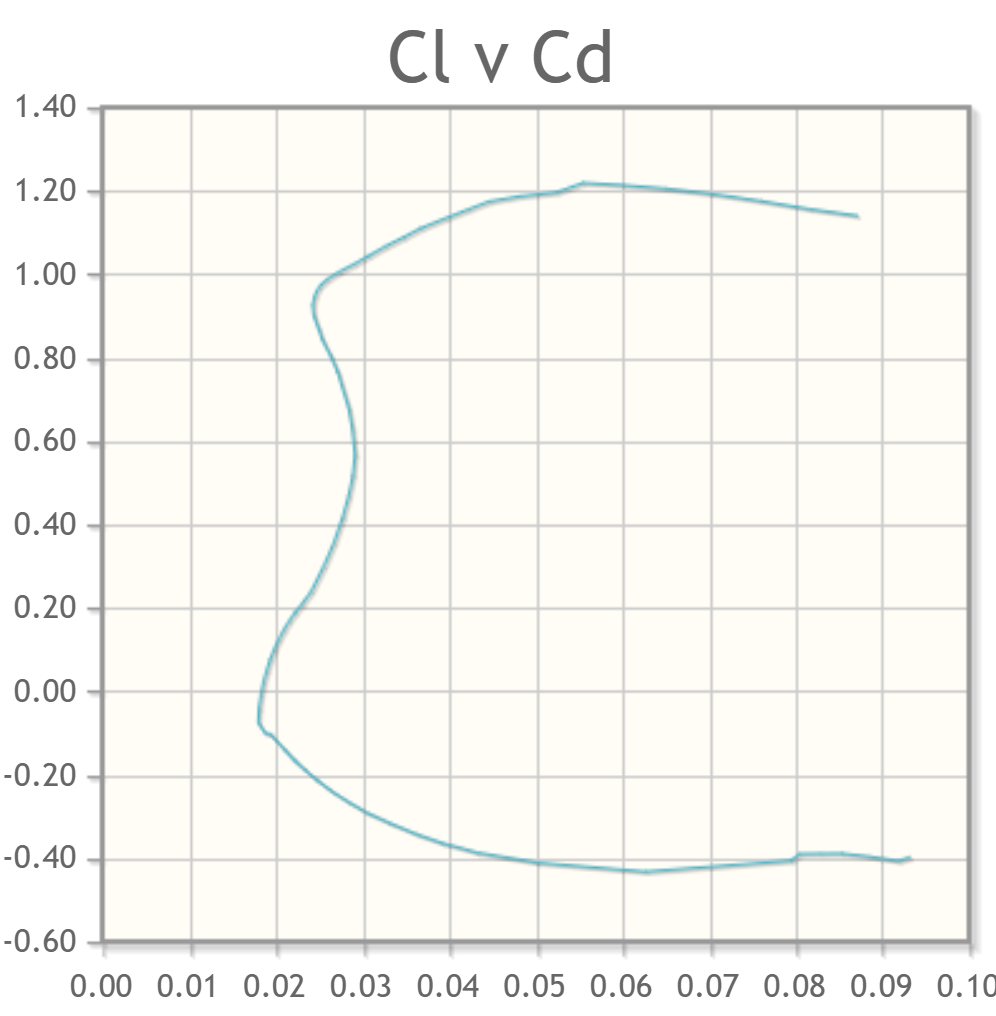
\includegraphics[width=0.4\textwidth]{Images/s2046 clvcd.png}}
    \hfil % Add some horizontal space between the figures
    \subfigure[Curve of $C_l$ and angle of attack]{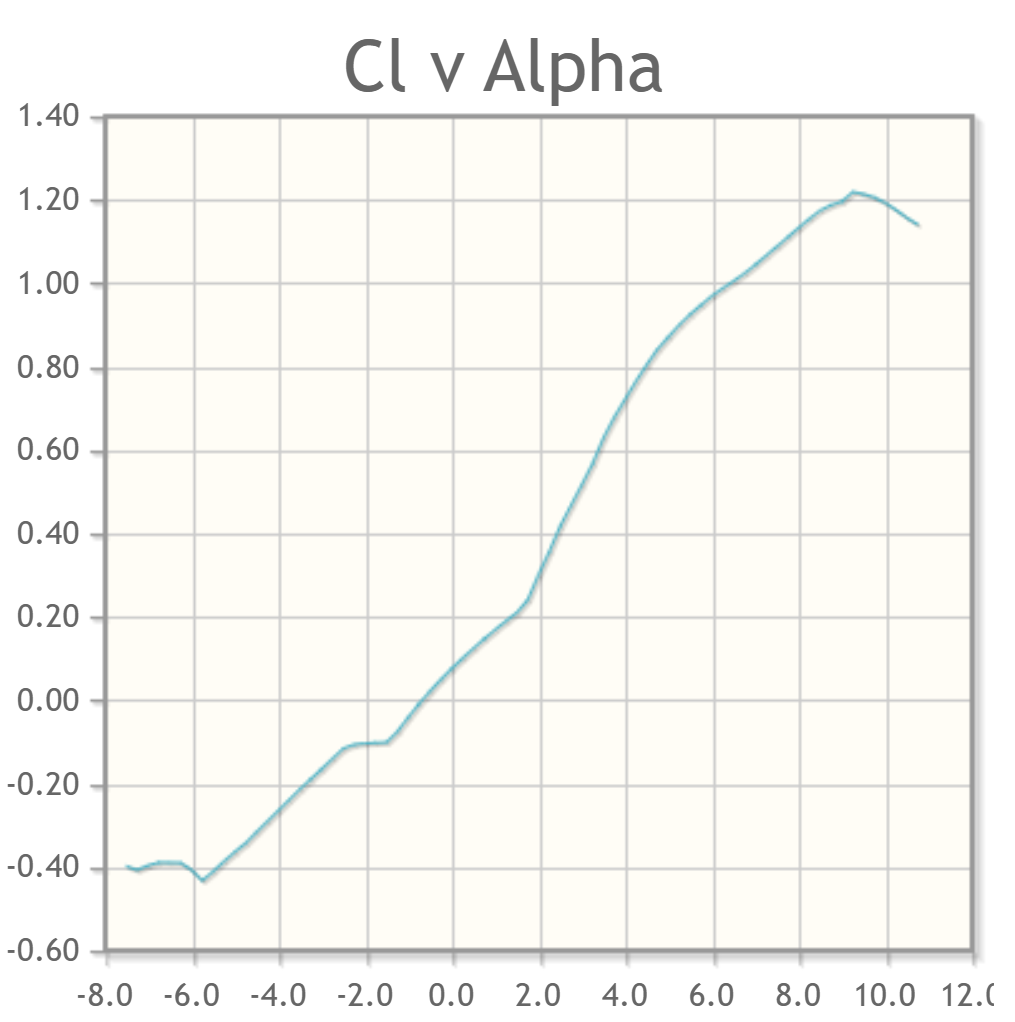
\includegraphics[width=0.4\textwidth]{Images/s2046 clvalpha.png}}    
    \caption{Selig 2046 airfoil aerodynamic coefficient Curve}
    \label{fig:aerodynamic coefficient Selig 2046}
\end{figure}

\begin{figure}
    \centering
    \subfigure[Curve of $C_l$ and $C_d$ aerodynamic coefficient]{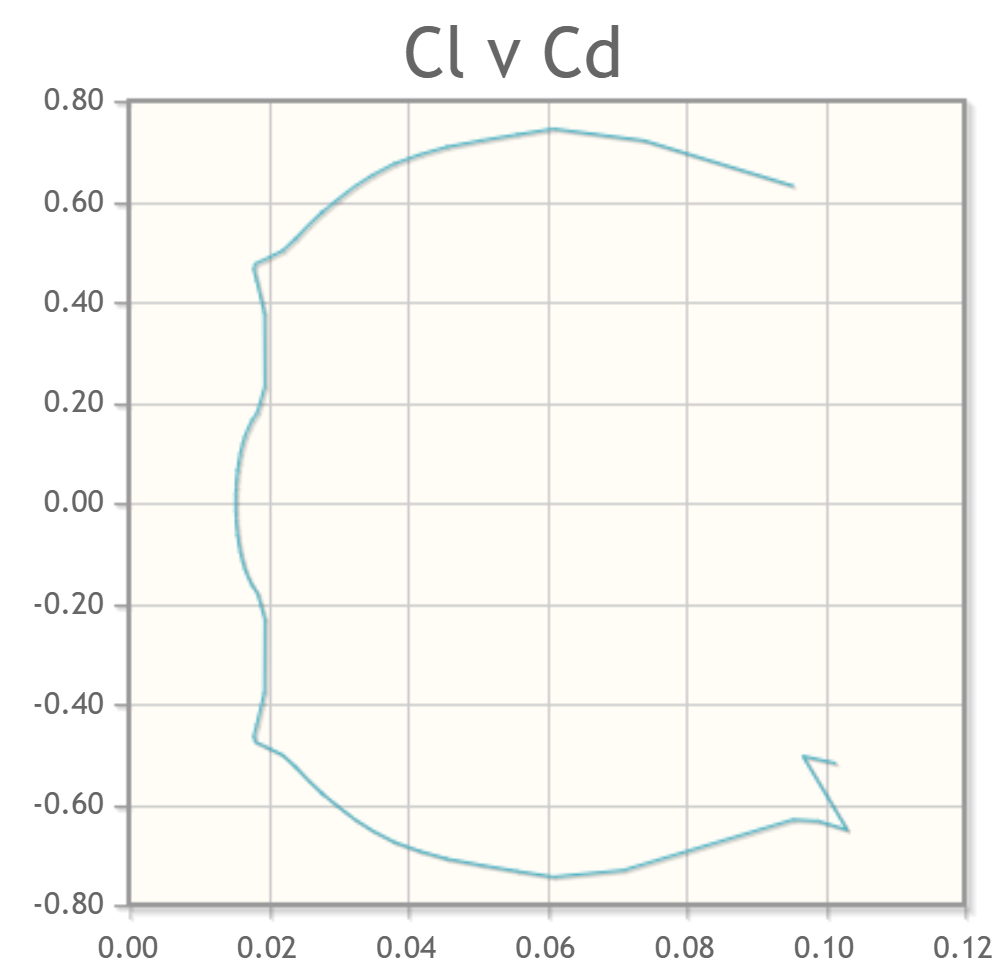
\includegraphics[width=0.4\textwidth]{Images/naca008 clvcd.png}}
    \hfil % Add some horizontal space between the figures
    \subfigure[Curve of $C_l$ and angle of attack]{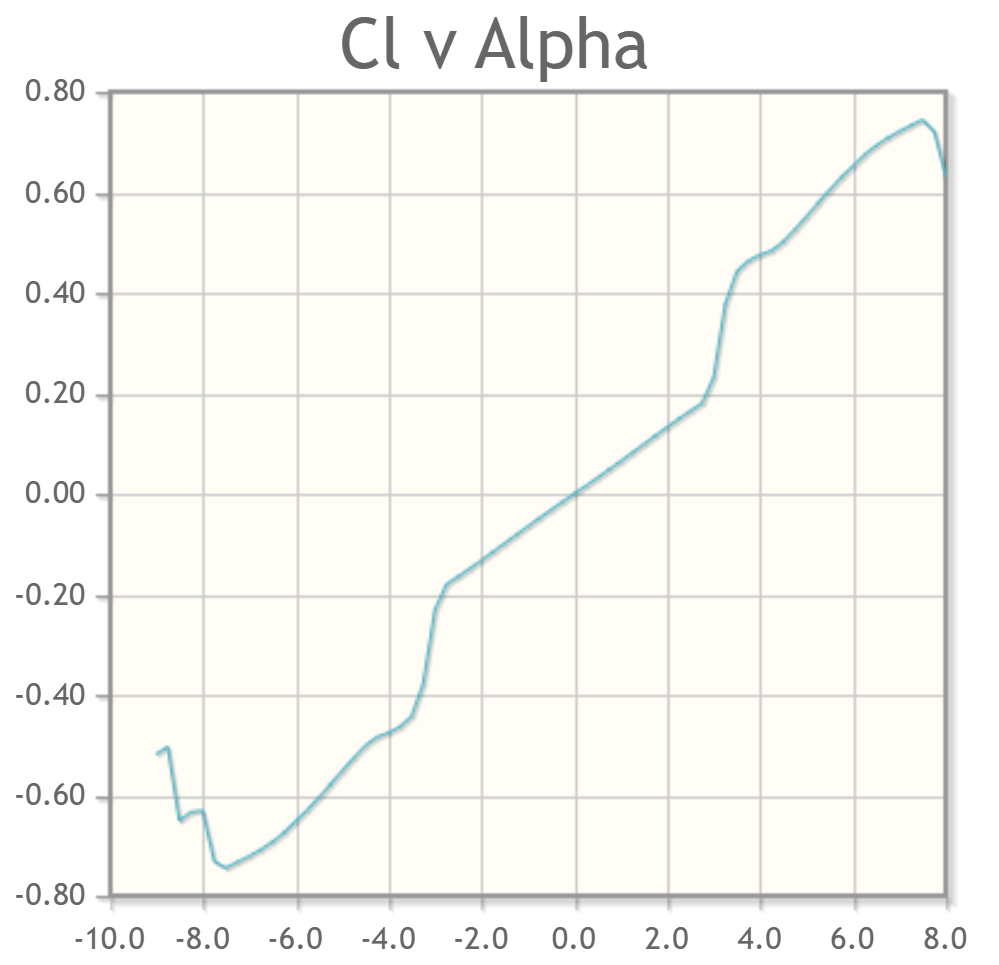
\includegraphics[width=0.4\textwidth]{Images/naca008 clvalpha.png}}    
    \caption{NACA 0008 airfoil aerodynamic coefficient Curve}
    \label{fig:aerodynamic coefficient naca 0008}
\end{figure}

\begin{table}[h]
\centering
\caption{C81 Data for Selig 2046 and NACA0008 Airfoils}
\label{tab:aero_coeffs}
\begin{tabular}{|c|c|c|c|c|c|c|}
\hline
\multirow{2}{*}{$\alpha$ (deg)} & \multicolumn{3}{c|}{S2046} & \multicolumn{3}{c|}{NACA0008} \\
\cline{2-7}
 & $C_{l\alpha}$ & $C_{d\alpha}$ & $C_{m\alpha}$ & $C_{l\alpha}$ & $C_{d\alpha}$ & $C_{m\alpha}$ \\
\hline
-2.50 & -0.1157 & 0.02003 & -0.0574 & -0.1649 & 0.01782 & -0.0122 \\
-2.25 & -0.1059 & 0.01961 & -0.0518 & -0.1490 & 0.01724 & -0.0119 \\
-2.00 & -0.1033 & 0.01962 & -0.0448 & -0.1325 & 0.01677 & -0.0112 \\
-1.75 & -0.1017 & 0.01941 & -0.0381 & -0.1157 & 0.01641 & -0.0104 \\
-1.50 & -0.1007 & 0.01888 & -0.0317 & -0.0988 & 0.01611 & -0.0093 \\
-1.25 & -0.0752 & 0.01807 & -0.0311 & -0.0818 & 0.01588 & -0.0081 \\
-1.00 & -0.0408 & 0.01816 & -0.0349 & -0.0649 & 0.01571 & -0.0067 \\
-0.75 & -0.0085 & 0.01838 & -0.0378 & -0.0483 & 0.01557 & -0.0052 \\
-0.50 & 0.0215 & 0.01867 & -0.0399 & -0.0319 & 0.01548 & -0.0035 \\
-0.25 & 0.0494 & 0.01903 & -0.0416 & -0.0158 & 0.01543 & -0.0018 \\
0.00 & 0.0757 & 0.01944 & -0.0428 & 0.0000 & 0.01541 & 0.0000 \\
0.25 & 0.1005 & 0.01991 & -0.0437 & 0.0158 & 0.01543 & 0.0018 \\
0.50 & 0.1243 & 0.02043 & -0.0445 & 0.0319 & 0.01548 & 0.0035 \\
0.75 & 0.1470 & 0.02100 & -0.0451 & 0.0483 & 0.01557 & 0.0052 \\
1.00 & 0.1689 & 0.02164 & -0.0456 & 0.0649 & 0.01570 & 0.0067 \\
1.25 & 0.1898 & 0.02235 & -0.0461 & 0.0818 & 0.01588 & 0.0081 \\
1.50 & 0.2099 & 0.02313 & -0.0465 & 0.0988 & 0.01611 & 0.0093 \\
1.75 & 0.2396 & 0.02418 & -0.0489 & 0.1158 & 0.01640 & 0.0104 \\
2.00 & 0.3003 & 0.02563 & -0.0566 & 0.1326 & 0.01677 & 0.0112 \\
2.25 & 0.3561 & 0.02679 & -0.0630 & 0.1490 & 0.01724 & 0.0119 \\
2.50 & 0.4167 & 0.02779 & -0.0696 & 0.1649 & 0.01782 & 0.0122 \\
\hline
\end{tabular}
\end{table}

Consider the implementation of control movable surfaces on the wings. For each wing, the main wings and horizontal tail wing need to be modeled separately.

\textbf{Main Wings:}
\begin{itemize}
    \item 3 elements
    \item Mid fixed wing, left and right wing with airfoil
    \item Each wing includes aileron control surfaces
    \item The aileron part constitutes 20\% of the modeled aerodynamic wing surface
    \item Considering the presence of the tip part, the actual ratio $\beta$ is 0.19
\end{itemize}

For the horizontal tail wing, which has an elevator control surface at the center of the aerodynamic wing surface, the horizontal surface is separated into 3 elements.

\textbf{Tail Wings:}
\begin{itemize}
    \item 5 elements
    \item Mid horizontal tail wing with elevator
    \item Left and right horizontal fixed tail wing
    \item 2 vertical tail wings with rudder
    \item The ratio $\beta$ is 30\% for both the horizontal and vertical tail wings
    \item Considering the presence of the tip part, the actual value of $\beta$ is 0.25
\end{itemize}

\begin{align}
    \beta_{\text{aileron}} = 0.1764 \\
    \beta_{\text{elevator}} = 0.3 \\
    \beta_{\text{rudder}} = 0.1050
\end{align}

\textbf{Aircraft Instruments}

The \texttt{aircraft\_node} in MBDyn represents the aircraft within a defined reference frame. By default, the positive x-direction aligns with the tail-to-nose axis, the positive z-direction aligns with the top-to-bottom axis, and the positive y-direction aligns with the rightward direction relative to the pilot. An optional orientation parameter can be specified for adjustments.

During simulation, various measures related to the aircraft's dynamics are accessible, such as airspeed, altitude, attitude, turn rate, and more. Additional data, like initial position, accelerations, and environmental conditions, are also available.

These parameters provide essential data for analyzing the aircraft's behavior and performance within the simulation environment.

\textbf{Body Velocity of Propeller:} In the part of force and moment element for the propeller, the airspeed of each propeller in the thrust direction is necessary to be used as the correction factor to generate the force and moment for each propeller. Considering the rotational movement of the drone itself and the influence of gust wings on the airspeed in complex test environments, using only the status data in the \textit{MassCenter} node is not accurate enough. A dummy node could be applied as sub-nodes for dynamic nodes, which could be used to build separate aircraft instruments in the position of every propeller. Use aircraft instruments to get the airspeed in the X-axis in the body frame of the drone for horizontal propellers and the airspeed in the Z-axis in the body frame of the drone for vertical propellers.

In addition to the aircraft instrument used for the propeller, another aircraft instrument is needed to be applied in the \textit{MassCenter} to monitor status information, such as airspeed, attitude angle, angular velocity, angular acceleration, etc. These data would be output by the output element part.

\subsubsection{General Elements}

To implement hardware delay in MBDyn, a scalar filter as a transfer function within General Elements is crucial.

This element models a scalar filter with the equation:
\begin{equation}
    A(s) y = B(s) u
\end{equation}
where \( A \) and \( B \) are polynomials of arbitrary order:
\begin{equation}
    y(s) = \frac{{b_0 s^{n_n} + b_1 s^{n_n-1} + \ldots + b_{n_n}}}{{a_0 s^{n_d} + a_1 s^{n_d-1} + \ldots + a_{n_d}}}u(s) 
\end{equation}
The filter must be proper, meaning \( n_d \) (output order) must be greater than or equal to \( n_n \) (input order). Polynomial \( A \) is monic (\( a_0 = 1 \)), and only coefficients from \( a_1 \) to \( a_n \) are needed. All coefficients of polynomial \( B \) must be provided, from \( b_0 \) to \( b_{n_n} \).

If a gain is supplied, all coefficients of \( B \) are multiplied by the gain.

Originally, input was required from a ScalarDof; now, it can also be taken from a drive, simplifying setup complexity.

In actual control situations, there is a hardware delay time that should be considered. In \cite{martello2021}, the actual delay time for movable surfaces has been provided. Referring to the data provided in \cite{battaini2020} on the Corona 939 Metal Gear servomotor \cite{CoronaServo} used for controlling surfaces, a time delay of 0.13 seconds is reported for movable surface control.

In \cite{battaini2022}, the actual delay time for the propeller has been provided. According to the experimental results in \cite{martello2021}, the delay time range is between 0.19 seconds and 0.27 seconds. For the MBDyn model, 0.25 seconds is chosen as the delay time applied in MBDyn.

These time delays for vertical propellers, horizontal propellers, and control surface actuation, as mentioned above, are integrated into the model using abstract nodes. The time delay for vertical propellers, which is upgraded in \cite{battaini2022}, is 0.015 seconds, and the time delay for horizontal propellers, which is designed in \cite{martello2021}, is 0.25 seconds.

Differential of Abstract Node and Scalar filter of Genel element is used to realize the delay effect in MBDyn. The transfer function is shown below:
\begin{equation}
    H(s) = \frac{\frac{1}{\tau}}{s+\frac{1}{\tau}}
\end{equation}
where \( \tau \) is a constant time value, set as the time delay value for each element.

Because the input command is the throttle of the motor, which needs to be computed to the actual angular velocity of the propeller used in the thrust or moment computation. The quadratic model between the angular velocity of the propeller and throttle command could be described as:
\begin{equation}
    th = a \cdot \Omega^2 + b \cdot \Omega \label{eq:th2Omega}
\end{equation}
where: \\
\(th\) is throttle command from the control system in percentage\\
\(\Omega\) is achieved angular velocity of the propeller
By equation (\ref{eq:th2Omega}), the relationship between angular velocity \( \Omega \) and throttle command \( th \) could be derived as:
\begin{equation}
    \Omega = \frac{- b + \sqrt{ b ^ 2 + 4 \cdot a \cdot th }}{2 \cdot a}
\end{equation}
The coefficients \( a \) and \( b \) of the vertical propeller, obtained with least square fitting in \cite{battaini2022}. To keep same in horizontal propeller, the coefficients \( a \) and \( b \) of horizontal propellers are also fitted using square fitting, are summarized in Table \ref{tab:Angular velocity against throttle quadratic model’s coefficients}. The curve between angular velocity and throttle command is shown in Figures \ref{fig:Motor dynamic response} and \ref{fig:Motor dynamic response2}.

\begin{table}[h]
    \centering
    \begin{tabular}{ccc}
        \hline
        Coefficients & Vertical & Horizontal \\
        \hline
        \( a \) & 2.71e-5 & 6.2972e-6 \\
        \( b \) & 1.73e-4 & 2.17e-2 \\
        \hline
    \end{tabular}
    \caption{Angular velocity against throttle quadratic model’s coefficients}
    \label{tab:Angular velocity against throttle quadratic model’s coefficients}
\end{table}

\begin{table}
    \centering
    \begin{tabular}{cccc}
    \hline
        $C_T$[-] & $C_Q$[-] & $C_P$[-] & $\tau$[1/s] \\
    \hline
        0.0186 & 0.00241 & 0.00241 & 0.015 \\
    \hline
    \end{tabular}
    \caption{Motor static coefficients and time constant; motor for vertical flight $KDE2315-XF2050$, 7x4.2 propeller.}
    \label{tab:Motor static coefficients}
\end{table}

\begin{table}[h]
    \centering
    \begin{tabular}{ccccc}
    \hline
    Start throttle & End throttle & Gain \( p \) & Time constant \( T \) & Fit percentage \\
    \hline
    40\% & 50\% & 18.9 & 0.24 & 79\% \\
    50\% & 60\% & 17.3 & 0.18 & 83\% \\
    60\% & 70\% & 17.8 & 0.25 & 80\% \\
    70\% & 80\% & 16.7 & 0.25 & 81\% \\
    \hline
    \end{tabular}
    \caption{Motor dynamic response identification results, motor for forward flight KDE2304XF-2350, 5x4.5 inch, 2 blades bullnose propeller.}
    \label{tab:Motor dynamic response1}
\end{table}

\begin{table}[h]
    \centering
    \begin{tabular}{ccccc}
    \hline
    Start throttle & End throttle & Gain \( p \) & Time constant \( T \) & Fit percentage \\
    \hline
    40\% & 50\% & 18.9 & 0.27 & 86\% \\
    50\% & 60\% & 17.3 & 0.23 & 85\% \\
    60\% & 70\% & 17.8 & 0.23 & 88\% \\
    70\% & 80\% & 16.7 & 0.26 & 87\% \\
    \hline
    \end{tabular}
    \caption{Motor dynamic response identification results, motor for vertical flight $KDE2315XF-2050$, 5x4.5 inch, 2 blades bullnose propeller.}
    \label{tab:Motor dynamic response2}
\end{table}

\begin{figure}
    \centering
    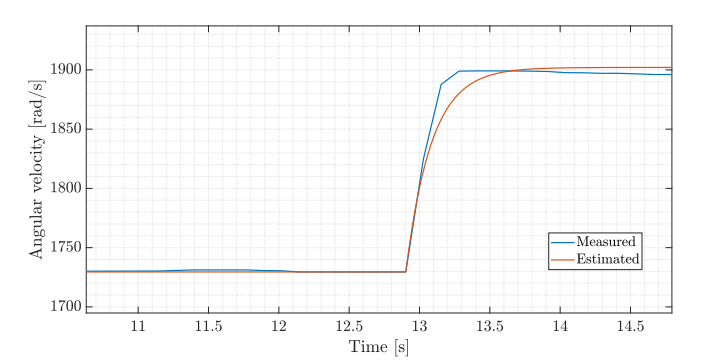
\includegraphics[width=0.75\linewidth]{Images/Motor dynamic response.png}
    \caption{Motor dynamic response, measured and identified response, motor powered from DC power supply at 14.8 V, motor for forward flight $KDE2304XF-2350$, 5x4.5 inch, 2 blades bullnose propeller.}
    \label{fig:Motor dynamic response}
\end{figure}

\begin{figure}
    \centering
    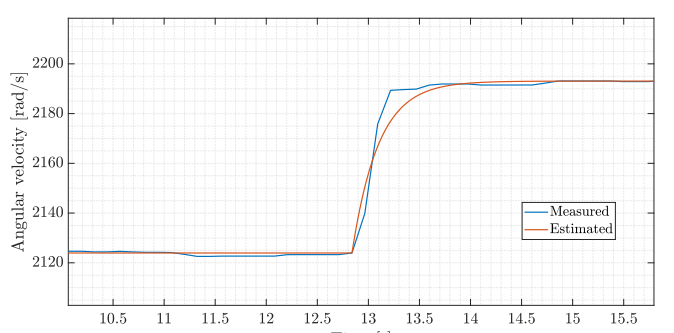
\includegraphics[width=0.75\linewidth]{Images/Motor dynamic response2.png}
    \caption{Motor dynamic response, measured and identified response, motor powered from DC power supply at 14.8 V, motor for vertical flight $KDE2315XF-2050$, 5x4.5 inch, 2 blades bullnose propeller.}
    \label{fig:Motor dynamic response2}
\end{figure}

\begin{figure}
    \centering
    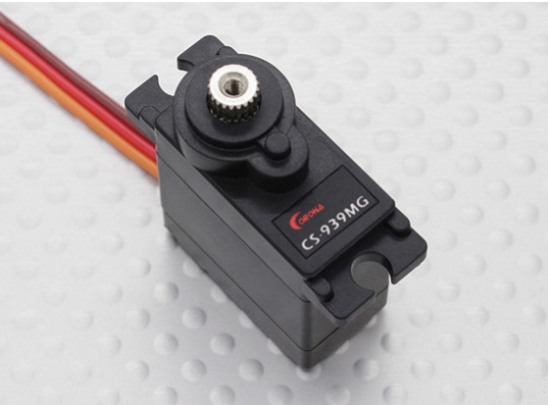
\includegraphics[width=0.5\linewidth]{Images/Corona 939 Metal Gear.png}
    \caption{Corona 939 Metal Gear}
    \label{fig:Corona 939 Metal Gear}
\end{figure}

\subsubsection{Gravity Elements}
To account for the influence of gravity force, a gravity element needs to be added. The 3D drive caller \textit{gravity\_acceleration} represents the gravity acceleration in the global reference frame.
This drone works below 100m, so the change of gravity acceleration with height could be neglected. The gravity acceleration is set to -9.81 m/s in the global Z-axis direction.

\subsubsection{Output Elements}
Output elements facilitate inter-process communication and can use specific communication means based on the type of simulation they are used for. They can transmit various types of data. In this simulation, the Stream output element is employed as a special element responsible for sending output to external processes via either \textit{local} or \textit{inet} sockets during batch or real-time simulations. It's worth noting that this topic is under development, so expect frequent changes, and please do not rely too heavily on backward compatibility. 

The Stream output allows MBDyn to send streamed outputs to remote processes during both batch and real-time simulations, using sockets either in the \textit{local} or \textit{inet} namespace. If the simulation runs in real-time using RTAI, RTAI mailboxes are used instead. The socket port is set to 10011, and \textit{send first} is enabled so that the control system could receive necessary airframe status information promptly. To obtain real-time flight status, including position, velocity, Euler angles, and angular velocity, data can be sourced from the \textit{MassCenter} node and its aircraft instruments. Additionally, to capture the force and moment acting on the center of mass, a total joint is utilized to link the \textit{MassCenter} node with the root. This arrangement allows for the representation of the rigid body within the root node, thereby facilitating the presentation of the force and moment acting on the center of mass through this joint. The total output information is shown in table \ref{tab:output element}.

\begin{table}
    \centering
    \begin{tabular}{ccc}
    \hline
        Output information & Number of ports & Unit\\
    \hline
        Position in global frame & 3 & $m$ \\
        Velocity in global frame & 3 & $m/s$ \\
        Acceleration in global frame & 3 & $m/s^2$ \\
        Euler angle in body frame & 3 & $rad$ \\
        Euler rates in body frame & 3 & $rad/s$ \\
        Euler angular acceleration & 3 & $rad/s^2$ \\
        Quaternions & 4 & 1 \\
        airspeed & 1 & $m/s$ \\
        angle of attack & 1 & $rad$ \\
        angle of slip & 1  & $rad$ \\
        Velocity in body frame & 3  & $rad/s$ \\
        altitude & 1 & $m$ \\
        Forces acted on mass of center of drone in body frame & 3 & $N$ \\
        Torques acted on mass of center of drone in body frame & 3 & $N \cdot m$ \\
    \hline
    \end{tabular}
    \caption{Output Information}
    \label{tab:output element}
\end{table}

\subsection{MBDyn Model Verification}
To validate the accuracy of the MBDyn model simulation, tests were conducted at an airspeed of 22 m/s. The default condition was tested with the aircraft fixed on the ground, having null attitude angles and null control surface deflections. In an additional case, the aircraft was positioned at a pitch angle of 5 degrees, and each control surface (aileron, elevator, rudder) was deflected by 5 degrees. Additionally, a rolling rotation velocity of 0.1 degrees per second was applied.

Expected values were manually calculated based on the same conditions using MBDyn simulation. Aerodynamic coefficients for each element were obtained according to the deflection angles set in the simulation. The total force and moment acting on the mass center were then calculated using dynamic pressure and measurements related to the mass center of each part. The table \ref{tab:Comparison of expect value and simulated results} presents the results, including both the simulation and manual expected computation:

\begin{sidewaystable}[htbp]
\centering
\begin{tabular}{|l|c|c|c|c|c|c|}
\hline
\textbf{Condition} & \textbf{$F_{x}$ (N)} & \textbf{$F_{y}$ (N)} & \textbf{$F_{z}$ (N)} & \textbf{$M_{x}$ (m*N)} & \textbf{$M_{y}$ (m*N)} & \textbf{$M_{z}$ (m*N)} \\
\hline
default condition & expect & -5.13E+00 & 0.00E+00 & 1.24E+02 & 0.00E+00 & -3.88E-01 \\
& Simulation & -5.14E+00 & 0.00E+00 & 1.24E+02 & -1.78E-15 & -3.88E-01 \\
& Error & 0.36\% & 0.00\% & 0.39\% & 0.00\% & 0.04\% \\
\hline
Pitch (5°) & expect & -1.05E+01 & 0.00E+00 & 2.10E+02 & 0.00E+00 & 1.09E-01 \\
& Simulation & -1.05E+01 & 0.00E+00 & 2.10E+02 & 3.46E-15 & 1.04E-01 \\
& Error & 0.01\% & 0.00\% & 0.00\% & 0.00\% & 4.68\% \\
\hline
Aileron (5°) & expect & -5.11E+00 & 3.56E-13 & 1.23E+02 & -6.69E+00 & -3.87E-01 \\
& Simulation & -5.11E+00 & 3.56E-13 & 1.23E+02 & -6.69E+00 & -3.87E-01 \\
& Error & 0.00\% & 0.00\% & 0.00\% & 0.00\% & 0.00\% \\
\hline
Elevator (5°) & expect & -5.16E+00 & 0.00E+00 & 1.26E+02 & 0.00E+00 & 1.74E+00 \\
& Simulation & -5.12E+00 & 0.00E+00 & 1.23E+02 & -1.78E-15 & -1.44E+00 \\
& Error & 0.00\% & 0.00\% & 0.00\% & 0.00\% & 0.00\% \\
\hline
Rudder (5°) & expect & -5.14E+00 & -3.54E-01 & 1.24E+02 & 3.15E-02 & -3.88E-01 \\
& Simulation & -5.14E+00 & -3.54E-01 & 1.24E+02 & 3.15E-02 & -3.88E-01 \\
& Error & 0.00\% & 0.00\% & 0.00\% & 0.00\% & -0.05\% \\
\hline
Rolling (0.1°/s) & expect & -5.14E+00 & 0.00E+00 & 1.24E+02 & -5.80E-02 & -3.88E-01 \\
& Simulation & -5.13E+00 & -1.08E+00 & 1.24E+02 & -5.62E-02 & -4.13E-01 \\
& Error & 0.36\% & 0.00\% & 0.39\% & 3.22\% & -6.08\% \\
\hline
\end{tabular}
\caption{Comparison of expect value and simulated results}
\label{tab:Comparison of expect value and simulated results}
\end{sidewaystable}

Comparison of the desired force and moment acting on the mass center with the simulation results reveals significant differences in the moment along the y-axis. This discrepancy may be attributed to errors in the main wing data or calculations. However, the results for all other metrics generally align with expectations. In the rolling movement section, the force and moment are affected by the non-linear relationship with the angle of attack. Consequently, there is a notable error compared to the simulation results, although it remains consistent with the manual computation. Figure \ref{fig:Force and moment monitored in clamp joint} illustrates the simulation results for force and moment in the global frame. Signals in the figure exhibit negligible noise caused by the simulation algorithm, which is lower than the error tolerance.

\begin{figure}[htbp]
    \centering
    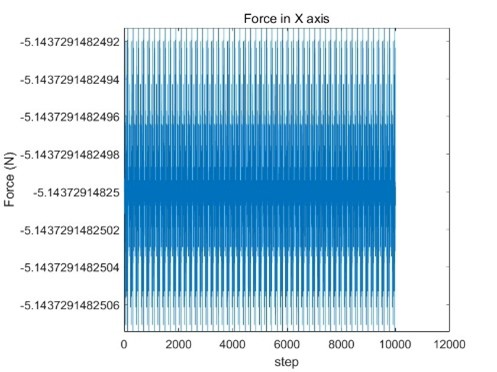
\includegraphics[width=0.45\textwidth]{Images/Vertify init/Picture1.jpg}
    \hfil
    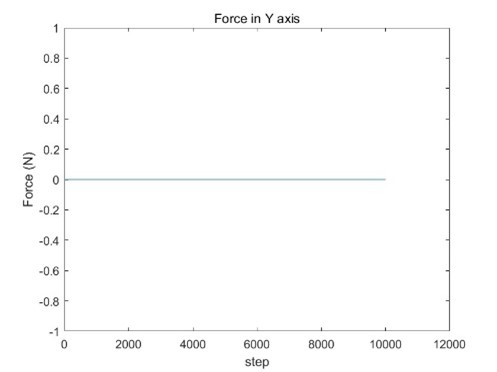
\includegraphics[width=0.45\textwidth]{Images/Vertify init/Picture2.jpg}
    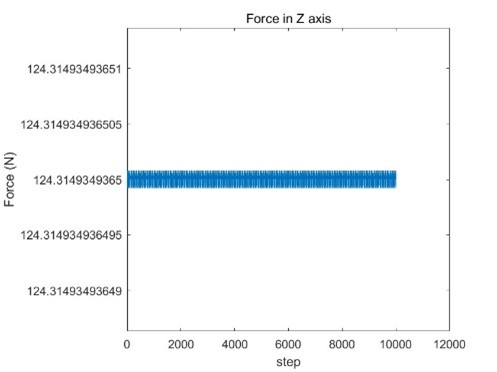
\includegraphics[width=0.45\textwidth]{Images/Vertify init/Picture3.jpg}
    \hfil
    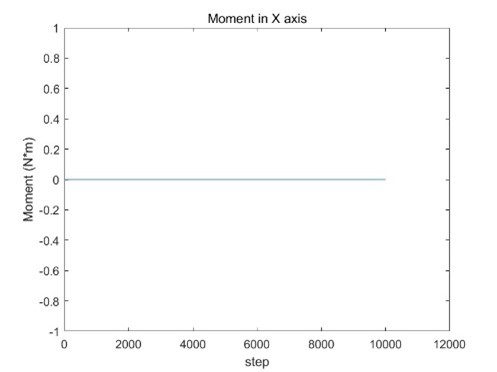
\includegraphics[width=0.45\textwidth]{Images/Vertify init/Picture4.jpg}
    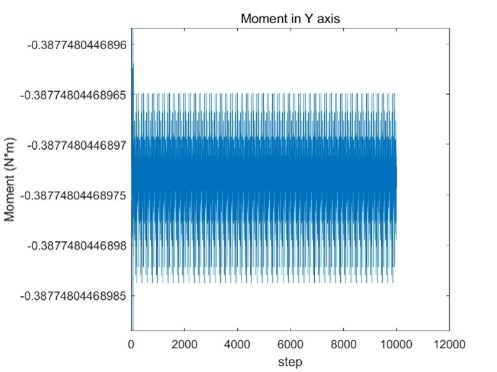
\includegraphics[width=0.45\textwidth]{Images/Vertify init/Picture5.jpg}
    \hfil
    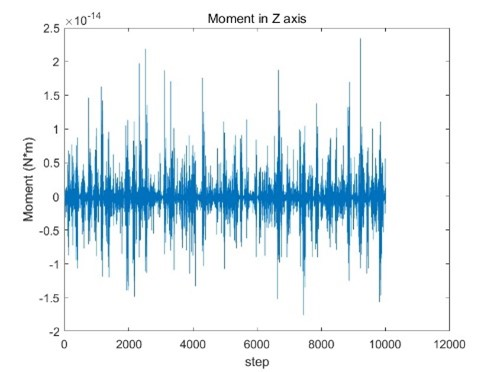
\includegraphics[width=0.45\textwidth]{Images/Vertify init/Picture6.jpg}
    \caption{Force and moment signal noise monitored in \textit{MassCenter} clamp joint}
    \label{fig:Force and moment monitored in clamp joint}
\end{figure}


\chapter{Integration and Control of Subsystems}

This chapter outlines the integration process between MBDyn and \textit{Simulink}, relevant concepts in \textit{Simulink} and control theory, and the architecture of the \textit{Simulink} control system. Following construction, the foundational control system is evaluated, and the typical control responses are examined.

\section{Concepts of Reference Frames and Rotation}

In aerospace engineering and navigation, a comprehensive grasp of reference frames and rotational principles is indispensable for accurately characterizing object and vehicle movements. These concepts underpin navigation, control, and simulation across various domains.

\subsection[Global Navigation Frame N]{Global Navigation Frame $\overrightarrow{\mathcal{N}}$}

The global navigation frame establishes a universal reference for delineating an object's motion relative to the Earth's surface. Typically, it is defined using Earth-centered coordinates like latitude, longitude, and altitude. Notable instances encompass the Earth-Centered, Earth-Fixed (ECEF) frame and the Geodetic frame. This frame furnishes a steadfast benchmark for navigation systems, enabling precise object localization and tracking across expansive geographic regions.

\subsection[Local Vertical Frame (NED)]{Local Vertical Frame (NED) $\mathcal{N}$}

The local vertical frame, also referred to as the North-East-Down (NED) frame, serves as a localized reference frame extensively employed in aircraft navigation and control. Centered at the vehicle's position, it aligns its $x$-axis with north, $y$-axis with east, and $z$-axis with the downward direction toward the Earth's center. Facilitating navigation and control algorithms, the NED frame provides an intuitive reference for elucidating the vehicle's motion in relation to its environment.

\subsection[Vehicle Body Frame]{Vehicle Body Frame $\mathcal{B}$}

The vehicle body frame serves as a reference frame fixed to the vehicle's structure. Aligned with the vehicle's movements and rotations, it provides a convenient framework for describing its motion and dynamics. Typically, the $x$-, $y$-, and $z$-axes of the body frame correspond to the vehicle's longitudinal, lateral, and vertical axes, respectively. Crucial for analyzing and managing the vehicle's motion, the body frame offers a reference relative to which forces and torques can be computed and applied.

\subsection[Wind Frame]{Wind Frame $\mathcal{W}$}

The wind frame constitutes a reference frame moving with the air mass surrounding the vehicle. It proves particularly valuable for scrutinizing aerodynamic forces and moments acting on an aircraft. In the wind frame, the $x$-axis aligns with the direction of the relative wind, the $y$-axis is perpendicular to the relative wind in the horizontal plane, and the $z$-axis points upward. Facilitating precise analysis of the vehicle's aerodynamic performance, the wind frame accommodates considerations of wind effects on its motion.

\begin{figure}
    \centering
    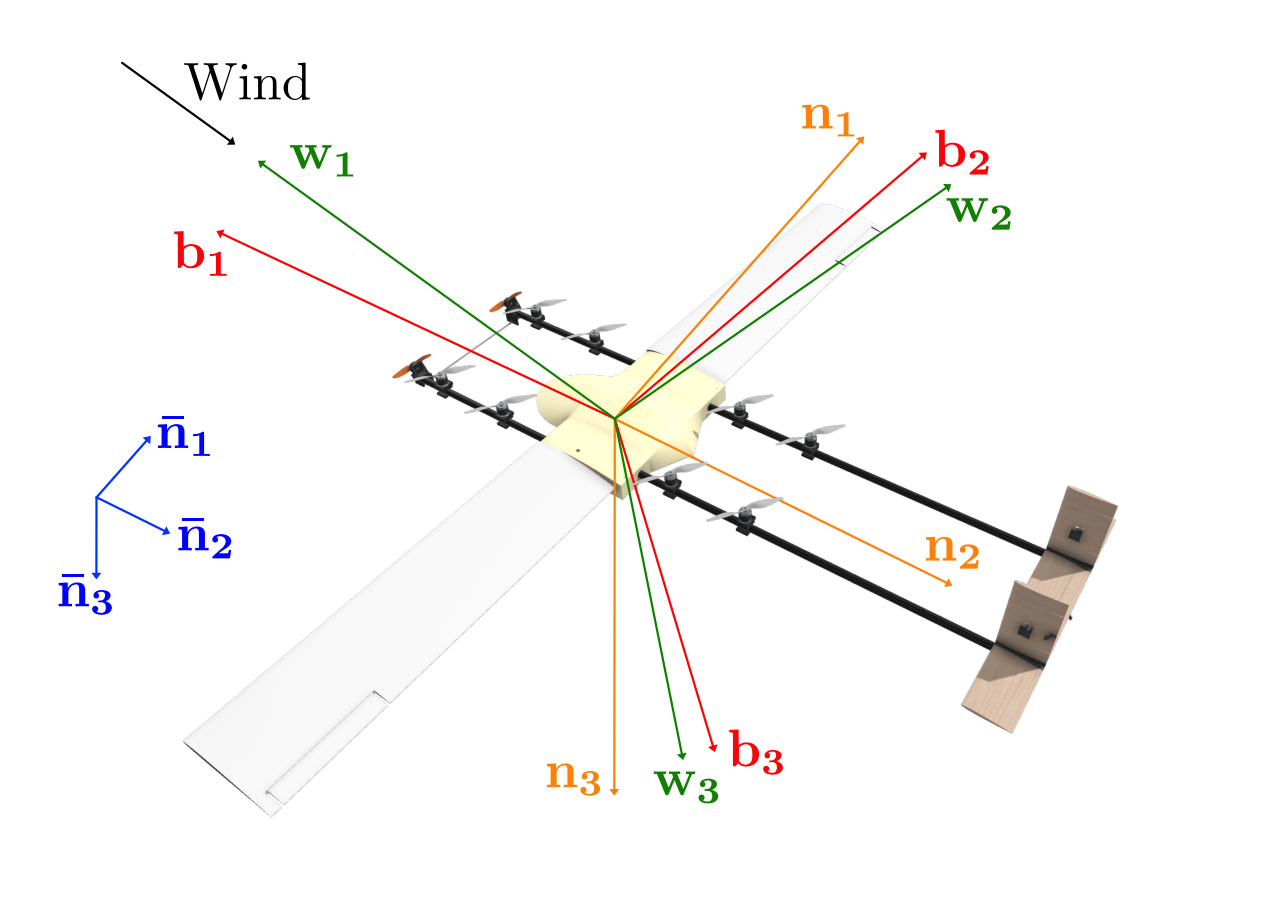
\includegraphics[width=0.8\linewidth]{Images/reference_frame.png}
    \caption{Schematic representation of reference frames.}
    \label{fig:reference_frames}
\end{figure}

\subsection{Rotation Formalism}

Rotation formalism is used to represent the orientation of an object or coordinate frame relative to another frame. Common representations include Euler angles, time derivatives of Euler angles, and quaternions.

\subsubsection{Euler Angles}
The Euler angles (called roll \(\phi\), pitch \(\theta\) and yaw \(\psi\)) are three independent angular quantities able to describe the 3D orientation of an object, using two sets of reference frames: an inertial Earth-fixed one and a body one, rigidly attached to the object. The Euler angles define the transformation of the components of a generic vector between two sets of axes. A vector \(\mathbf{v}_A\) in the initial reference frame \(A\) can be rotated into the reference frame \(B\) obtaining \(\mathbf{v}_B\), with the rotation matrix \(\mathbf{R}_{B}^{A}\):
\begin{equation}
    \mathbf{v}_B = \mathbf{R}_{A}^{B} \mathbf{v}_A. \label{eq:rotation_matrix}
\end{equation}
Any arbitrary attitude is obtained by an ordered sequence of three consecutive rotations around each axis of an orthogonal frame; the rotation around the \(x\) axis can be described with matrix \(R_x(\phi)\):
\begin{equation}
    R_X(\phi) = \begin{bmatrix} 
        1 & 0 & 0 \\ 
        0 & \cos \phi & \sin \phi \\ 
        0 & -\sin \phi & \cos \phi 
    \end{bmatrix}, \label{eq:rotation_x}
\end{equation}
while, in similar fashion the rotation around \(y\) and \(z\) are described respectively with rotation matrices \(R_y(\theta)\), \(R_z(\psi)\):
\begin{align}
    R_Y(\theta) &= \begin{bmatrix} 
        \cos \theta & 0 & -\sin \theta \\ 
        0 & 1 & 0 \\ 
        \sin \theta & 0 & \cos \theta 
    \end{bmatrix}, \label{eq:rotation_y} \\
    R_Z(\psi) &= \begin{bmatrix} 
        \cos \psi & \sin \psi & 0 \\ 
        -\sin \psi & \cos \psi & 0 \\ 
        0 & 0 & 1 
    \end{bmatrix}. \label{eq:rotation_z}
\end{align}
In aircraft dynamics, the generic attitude of the vehicle is obtained by the so-called rotation sequence 321: the attitude of the body axes \(B\) (always aligned with the aircraft) with respect to a non-rotating NED \(N\) reference frame, is obtained by a first rotation about the \(z\) axis of an angle \(\psi\), then a rotation about the \(y\) axis of an angle \(\theta\), and finally a rotation about the \(x\) axes of an angle \(\phi\). The final rotation matrix from \(N\) to \(B\) is obtained by the ordered multiplication of the previous rotation matrices (equations \eqref{eq:rotation_x}, \eqref{eq:rotation_y}, and \eqref{eq:rotation_z}); it is called Euler rotation matrix and has the following expression:
\begin{equation}
    \mathbf{T}_{N}^{B}(\phi, \theta, \psi) = \begin{bmatrix} 
        C_{\theta}C_{\psi} & C_{\theta}S_{\psi} & -S_{\theta} \\ 
        S_{\phi}S_{\theta}C_{\psi} - C_{\phi}S_{\psi} & S_{\phi}S_{\theta}S_{\psi} + C_{\phi}C_{\psi} & S_{\phi}C_{\theta} \\ 
        C_{\phi}S_{\theta}C_{\psi} + S_{\phi}S_{\psi} & C_{\phi}S_{\theta}S_{\psi} - S_{\phi}C_{\psi} & C_{\phi}C_{\theta} 
    \end{bmatrix}, \label{eq:euler_rotation_matrix}
\end{equation}
where \(C_{\alpha} = \cos(\alpha)\) and \(S_{\alpha} = \sin(\alpha)\) for the sake of brevity.
The roll angle \(\phi\), the pitch angle \(\theta\), and the yaw angle \(\psi\) are grouped in the vector \(\boldsymbol{\alpha}_e\), which uniquely describes the aircraft’s attitude in space with respect to the NED reference frame \(N\):
\begin{equation}
    \boldsymbol{\alpha}_e = \begin{bmatrix} 
        \phi \\ 
        \theta \\ 
        \psi 
    \end{bmatrix}. \label{eq:euler_angles_vector}
\end{equation}

\subsubsection{Time derivatives of Euler angles}
The attitude of an aircraft changes with time when the aircraft maneuvers. The Euler angle rates are a function of the Euler angles and body-axis angular rates. The components of the angular velocity measured in the body frame \(\omega_B\) are the roll rate \(p\), pitch rate \(q\), and yaw rate \(r\):
\begin{equation}
    \boldsymbol{\omega}_B = \begin{bmatrix} 
        p \\ 
        q \\ 
        r 
    \end{bmatrix}. \label{eq:angular_velocity}
\end{equation}
The rate of change of Euler angles is related to \(\omega_B\) by the following equation:
\begin{equation}
    \dot{\boldsymbol{\alpha}}_e = E^{-1} \boldsymbol{\omega}_B, \label{eq:euler_angle_rate}
\end{equation}
with \(E^{-1}\) being the inverse of matrix \(E\), whose expressions are given by:
\begin{align}
    E(\phi, \theta) &= \begin{bmatrix} 
        1 & 0 & -\sin \theta \\ 
        0 & \cos \phi & \sin \phi \cos \theta \\ 
        0 & -\sin \phi & \cos \phi \cos \theta 
    \end{bmatrix}, \label{eq:matrix_E} \\
    E^{-1}(\phi, \theta) &= \begin{bmatrix} 
        1 & \sin \phi \tan \theta & \cos \phi \tan \theta \\ 
        0 & \cos \phi & -\sin \phi \\ 
        0 & \frac{\sin \phi}{\cos \theta} & \frac{\cos \phi}{\cos \theta} 
    \end{bmatrix}. \label{eq:matrix_E_inverse}
\end{align}
It can be seen that matrix \(E\) is singular for pitch angles of \(\pm 90^\circ\); this singularity is called gimbal lock and can be avoided using quaternions.
\subsubsection{Quaternions}
A quaternion \( q \) is a parametrization of the four-dimensional unit sphere that can be used to represent the orientation of a rigid body or a coordinate frame in three-dimensional space:
\begin{equation}
    q = \begin{bmatrix} 
        q_0 \\ 
        q_1 \\ 
        q_2 \\ 
        q_3 
    \end{bmatrix}, \quad ||q|| = 1.    
\end{equation}
The quaternion elements generate the following rotation matrix (analogous to the one expressed in Equation \eqref{eq:euler_rotation_matrix} in terms of Euler angles):
\begin{equation}
\mathbf{T}_{N}^{B} = \begin{bmatrix} 
    q_0^2 + q_1^2 - q_2^2 - q_3^2 & 2(q_1q_2 + q_0q_3) & 2(q_1q_3 - q_0q_2) \\ 
    2(q_1q_2 - q_0q_3) & q_0^2 - q_1^2 + q_2^2 - q_3^2 & 2(q_2q_3 + q_0q_1) \\ 
    2(q_1q_3 + q_0q_2) & 2(q_2q_3 - q_0q_1) & q_0^2 - q_1^2 - q_2^2 + q_3^2 
\end{bmatrix}.
\end{equation}
The Euler angles \(\phi\), \(\theta\), and \(\psi\) can be obtained from the elements of the quaternion expressing the aircraft’s orientation with respect to a non-rotating frame through
\begin{align}
    \phi &= \tan^{-1} \left( \frac{2q_3q_4 - 2q_1q_2}{2q_1^2 - 1 + 2q_4^2} \right), \label{eq:euler_angles_phi} \\
    \theta &= -\sin^{-1}(2q_2q_4 + 2q_1q_3), \label{eq:euler_angles_theta} \\
    \psi &= \tan^{-1} \left( \frac{2q_2q_3 - 2q_1q_4}{2q_1^2 - 1 + 2q_2^2} \right). \label{eq:euler_angles_psi}
\end{align}
The quaternion conjugate, denoted by \( (\cdot)^* \), can be used to swap the frames described by an orientation. To follow the previous example, the orientation of frame \( B \) with respect to frame \( A \) can be described by the quaternion \( q_{AB} \), and its conjugate \( q_{AB}^* \) describes the orientation of frame \( A \) relative to frame \( B \) (\( q_{BA} \)), like in the following equation:
\begin{equation}
q_{AB}^* = q_{BA} = \begin{bmatrix} 
    q_0 \\ 
    -q_1 \\ 
    -q_2 \\ 
    -q_3 
\end{bmatrix}.
\end{equation}

The quaternion product, denoted as \( (\otimes) \), is used to describe successive rotations and can be determined using the Hamilton rule, as expressed by Equation \eqref{eq:qac}. The quaternion product is not commutative.
\begin{equation}
q_{AC} = q_{BC} \otimes q_{AB} = \begin{bmatrix} 
    a_0 \\ 
    a_1 \\ 
    a_2 \\ 
    a_3 
\end{bmatrix} \otimes \begin{bmatrix} 
    b_0 \\ 
    b_1 \\ 
    b_2 \\ 
    b_3 
\end{bmatrix} = \begin{bmatrix} 
    a_1b_1 - a_2b_2 - a_3b_3 - a_4b_4 \\ 
    a_1b_2 + a_2b_1 + a_3b_4 - a_4b_3 \\ 
    a_1b_3 - a_2b_4 + a_3b_1 + a_4b_2 \\ 
    a_1b_4 + a_2b_3 - a_3b_2 + a_4b_1 
\end{bmatrix}.  \label{eq:qac}
\end{equation}
A three-dimensional vector can be rotated by a quaternion using Equation \eqref{eq:vb_qbc} by appending a zero as the first element of the vector to make it dimensionally consistent with quaternions:
\begin{equation}
    \mathbf{v}_B = q_{AB} \otimes \mathbf{v}_A \otimes q_{AB}^*,    \label{eq:vb_qbc}
\end{equation}
where \( \mathbf{v}_A \) and \( \mathbf{v}_B \) are the same vector described in frame A and frame B, respectively.

Finally, the quaternion derivative describing the rate of change of orientation of the Earth frame relative to the body frame can be calculated by the equation:
\begin{equation}
\dot{q}_{BE} = \frac{1}{2} q_{BE} \otimes \boldsymbol{\omega}, \quad \text{where} \quad \boldsymbol{\omega} = \begin{bmatrix} 0 \\ \omega_B \end{bmatrix}, \label{eq:q_BE}
\end{equation}
Resolving Equation \eqref{eq:q_BE} leads to
\begin{equation}
    \begin{bmatrix} 
        \dot{q}_1 \\ 
        \dot{q}_2 \\ 
        \dot{q}_3 \\ 
        \dot{q}_4 
    \end{bmatrix} = \frac{1}{2} \begin{bmatrix} 
        0 & -p & -q & -r \\ 
        p & 0 & r & -q \\ 
        q & -r & 0 & p \\ 
        r & q & -p & 0 
    \end{bmatrix} \begin{bmatrix} 
        q_1 \\ 
        q_2 \\ 
        q_3 \\ 
        q_4 
    \end{bmatrix}.    
\end{equation}

\section{Integration with Airframe in MBDyn}

MBDyn offers a variety of modules for interfacing with different software platforms, such as \textit{Simulink}, enabling real-time data exchange with MBDyn to maintain consistent configurations in the model. In the \textit{Simulink} model, the time step is set to \(10^{-3}\) seconds.

\begin{sidewaysfigure}
    \centering
    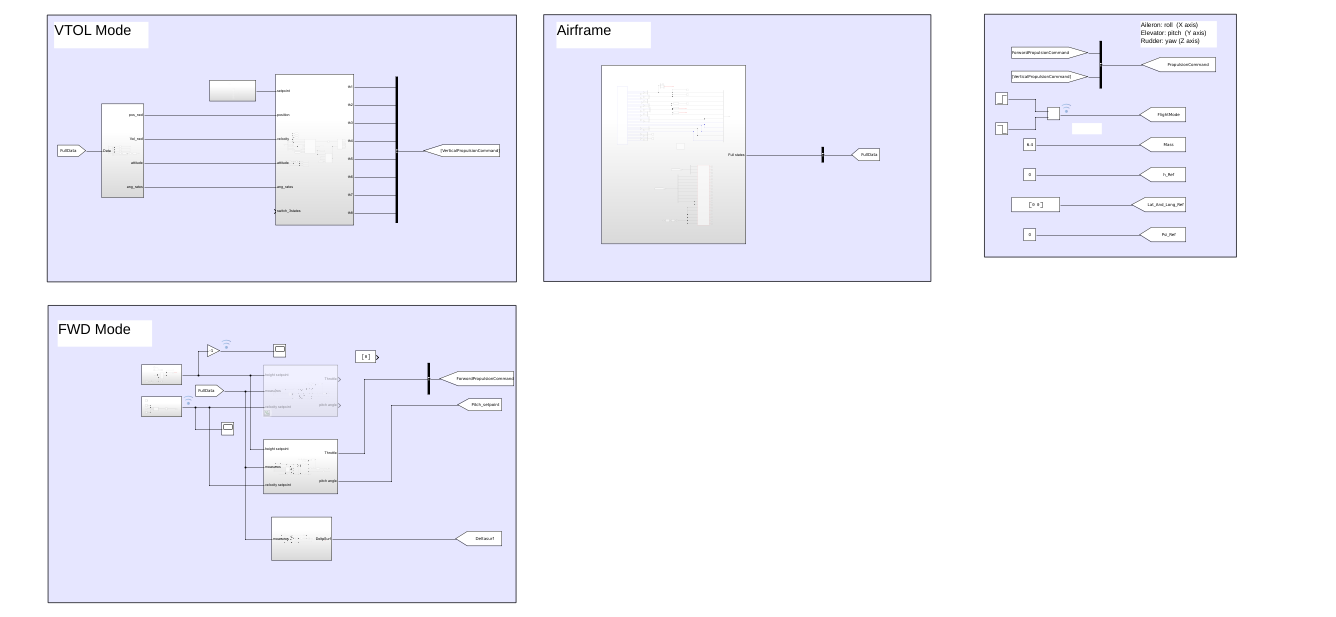
\includegraphics[width=1\linewidth]{Images/SImulink_overview.png}
    \label{fig:Simulink_overview}
    \caption{Overview of the \textit{Simulink} Control System}
\end{sidewaysfigure}

\section{\textit{Simulink} Control System}

The \textit{Simulink} model remains consistent with the description provided in \cite{battaini2022}, featuring both multi-copter and fixed-wing modes within the control system. Inputs and outputs have been adjusted for communication with the MBDyn model.

The \textit{Simulink} module sends 13 control command signals to the MBDyn system, comprising 1-3 ports for movable surfaces (aileron, elevator, rudder), 4-11 ports for throttle command for vertical motors, and 12-13 ports for throttle command for horizontal motors. Conversely, the \textit{Simulink} module receives status information from the MBDyn module, encompassing a total of 35 received signals as outlined in Table \ref{tab:output element}. The integrated MBDyn send and receive module in \textit{Simulink} is depicted in Figure \ref{fig:Simulink_Block_connect_with_MBDyn}.

Since all data output from the MBDyn simulation is in either the global frame, body frame, or wind frame, within the \textit{Simulink} control system, all data is utilized in the global navigation frame, vehicle body frame, or wind frame. Consequently, data is rotated to the corresponding frame using a gain block with a value of -1 before being utilized in the control system.

\begin{sidewaysfigure}
  \centering
  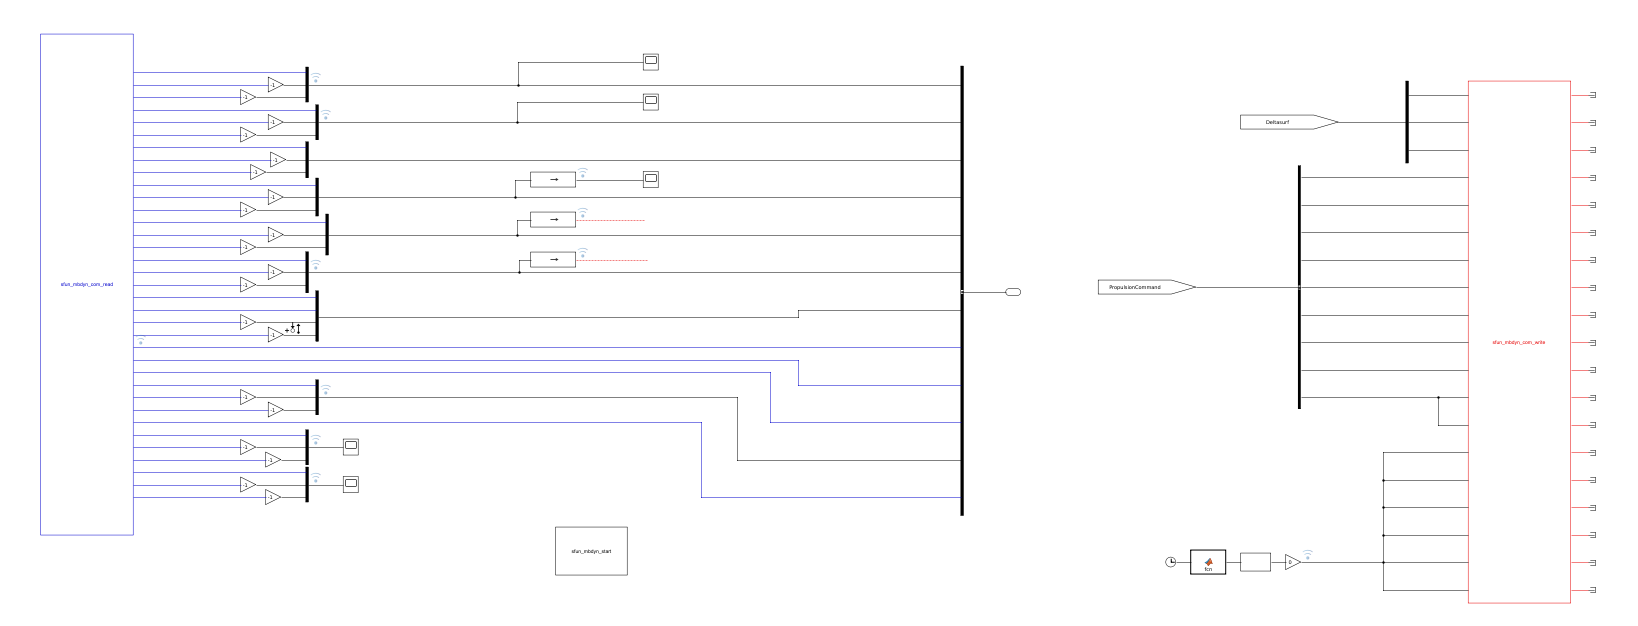
\includegraphics[width=1\linewidth]{Images/airframe.png}
  \caption{Integration of Simulink Block with MBDyn}
  \label{fig:Simulink_Block_connect_with_MBDyn}
\end{sidewaysfigure}

\subsection{Multi-Copter Mode}

The multicopter controller architecture described in \cite{battaini2022} consists of standard cascaded loops with PID controllers derived from \cite{px4controller}. Four loops are present: on the body angular rates, on the attitude angles, on the inertial velocity, and on the inertial position. The structure of the controller \cite{Px4AutopilotWebsite} is depicted in Figure \ref{fig:Multicopter_controller}: a proportional controller \(P\) is used for position and attitude control, while a proportional, integral, and derivative (PID) controller is used for rates and velocity control. The final outputs of the controller are the vertical body force \(T\) and body moments \(L\), \(M\), \(N\), which are converted into motor angular velocities \(\Omega\) with the pseudo-inverse of the mixer matrix \(\chi\), and then into throttle commands \(th\) with the relation \cite{Px4DiscussionForum}:

\begin{equation}
    th = a \Omega^2 + b \Omega, \label{eq:throttle}
\end{equation}

as found in Chapter \ref{ch:chapter1}.

\begin{figure}[h]
    \centering
    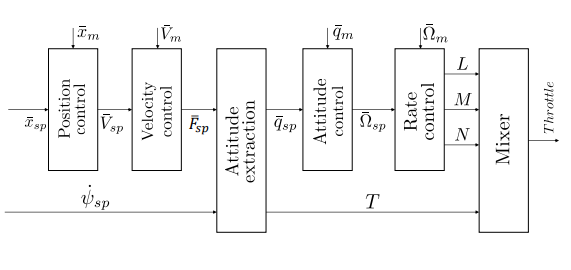
\includegraphics[width=0.9\linewidth]{Images/Multicopter controller.png}
    \caption{Multicopter controller.}
    \label{fig:Multicopter_controller}
\end{figure}

The Simulink implementation of the controller is depicted in Figure \ref{fig:VTOL_controller}. Three main subsystems are visible:

\begin{itemize}
    \item Position controller block, which calculates the body force \(T\) and the desired attitude from position/velocity setpoint;
    \item Attitude controller block, which calculates body moments \(L\), \(M\), \(N\) from attitude setpoint;
    \item Mixer block, which transforms force and moments into throttle commands.
\end{itemize}

The details of the position controller block are shown in Figure \ref{fig:position_controller}: including the position control, velocity control, and setpoint attitude extraction subsystems. Saturation limits are introduced to account for propulsion limits. An integral reset flag is added to avoid continuous error integration by the controller when the multi-rotor is not flying: if the thrust command value is below 20\%, the integration is stopped. There is a feed-forward term on the acceleration setpoint, and the constant force contribution of the weight is considered. The in-plane thrust suppression block manages the force contribution when the drone is on the ground: in this condition, the force is maintained at an idle value until the thrust command reaches 20\%. Additionally, during ALTITUDE MODE, the in-plane thrust suppression block cancels the horizontal component of the force.

The attitude controller block is depicted in Figure \ref{fig:attitude_controller}, composed of attitude and rate control with saturation limits and integral reset.

The attitude controller is based on \cite{brescianini2013nonlinear} and makes use of quaternions \([q_x, q_y, q_z, q_w]\). The drone is an under-actuated mechanical system since it has a lower number of control inputs than the number of degrees of freedom to be controlled: the force generated is oriented in the body vertical direction, so it can only accelerate along this axis. Therefore, the force setpoint \(\bar{F}_{\text{sp}}\) calculated by the velocity controller is transformed into a target orientation \(\bar{q}_{\text{sp}}\), such that the corresponding z-axis is aligned with the desired force.

\begin{sidewaysfigure}
  \centering
      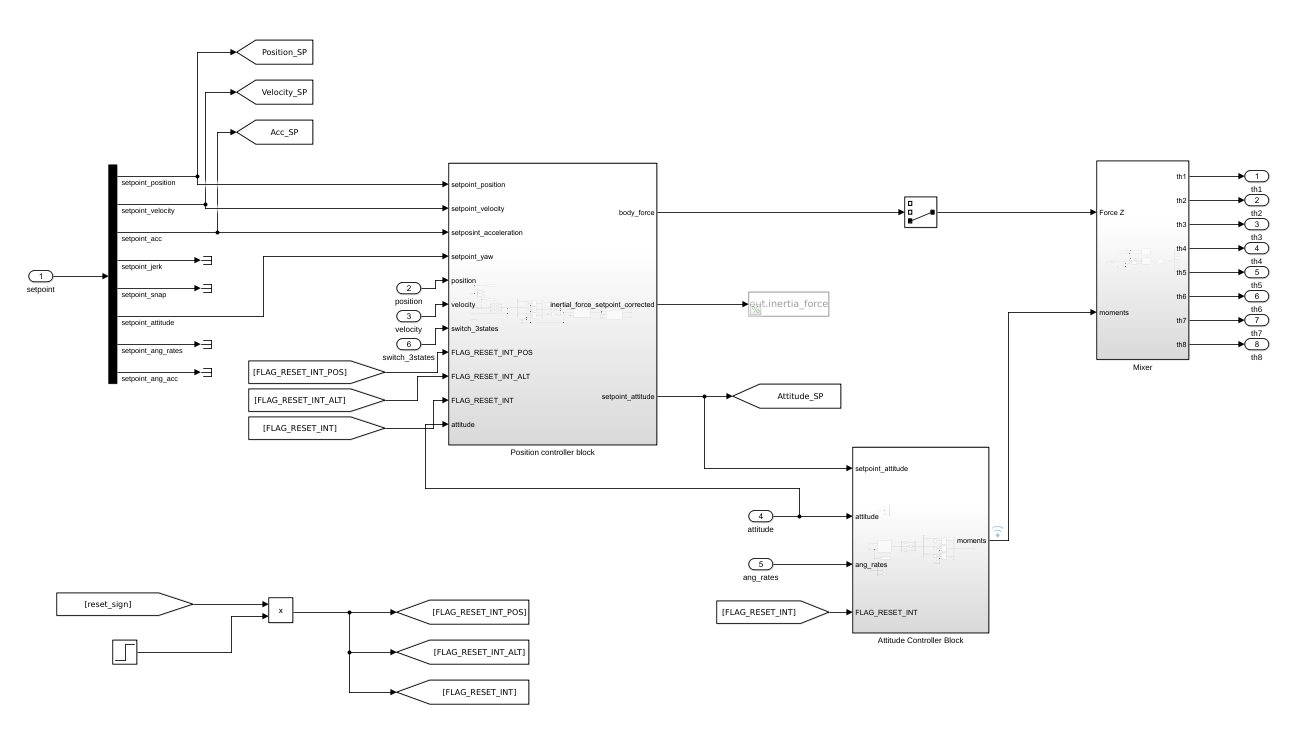
\includegraphics[width=1\linewidth]{Images/VTOL_controller.png}
      \caption{VTOL controller block}
      \label{fig:VTOL_controller}
\end{sidewaysfigure}

\begin{sidewaysfigure}
  \centering
      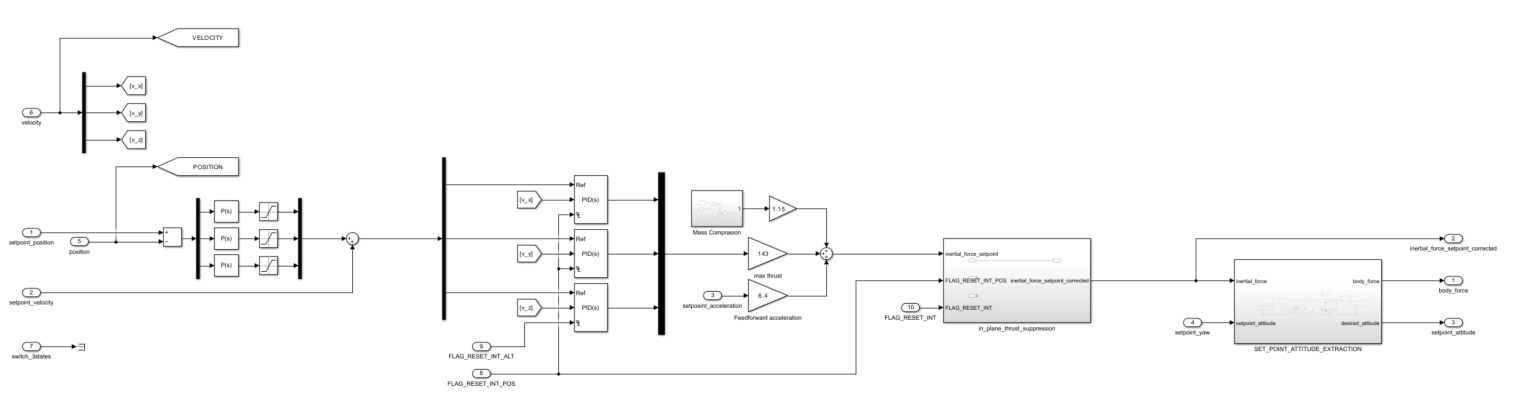
\includegraphics[width=1\linewidth]{Images/position_controller.png}
      \caption{Position controller block}
      \label{fig:position_controller}
\end{sidewaysfigure}

\begin{sidewaysfigure}
  \centering
      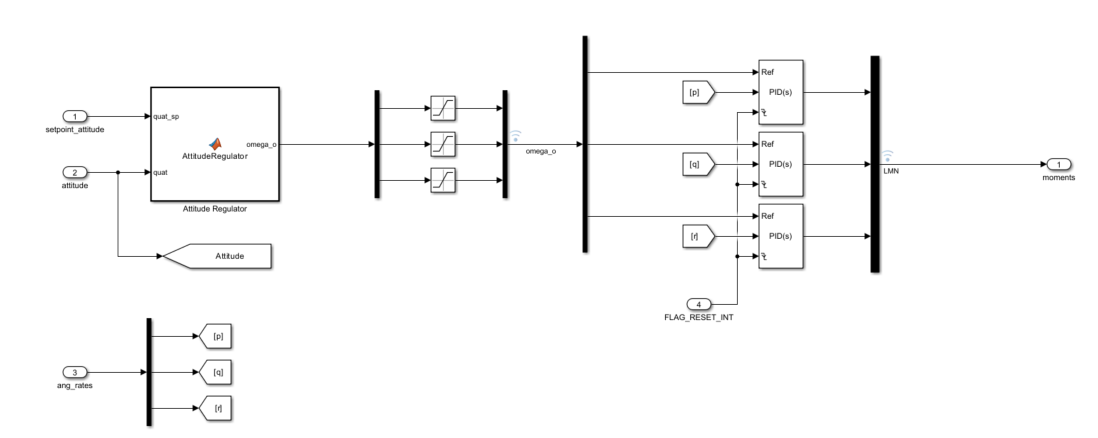
\includegraphics[width=1\linewidth]{Images/attitude_controller.png}
      \caption{Attitude controller block}
      \label{fig:attitude_controller}
\end{sidewaysfigure}

\begin{sidewaysfigure}
  \centering
      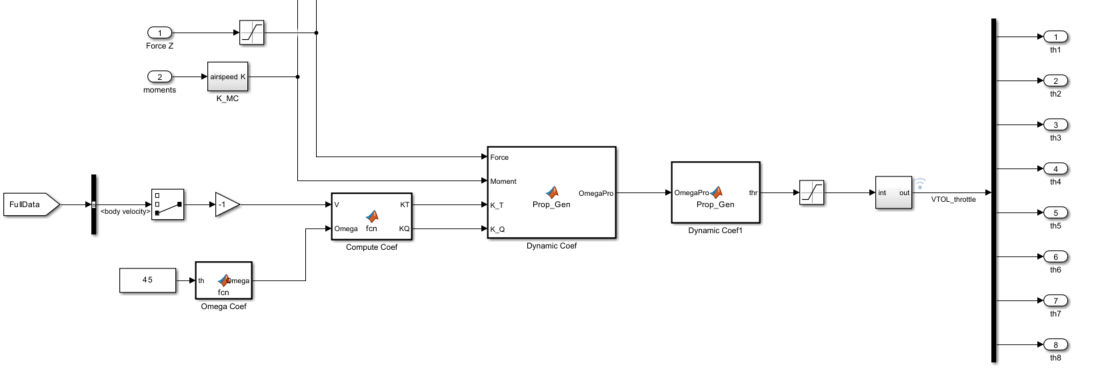
\includegraphics[width=1\linewidth]{Images/mixer_control.png}
      \caption{Mixer controller block}
      \label{fig:mixer_control}
\end{sidewaysfigure}

\subsubsection{Notch Filter}

Significant effort was dedicated to selecting proportional gains to strike a balance between tracking performance and minimizing vibrations. However, even after the tuning campaign, noticeable vibrations persisted. Visual analysis suggested that these vibrations originated in the wings and propagated throughout the entire vehicle. To confirm this hypothesis, a flight was conducted without wings, resulting in the absence of vibrations, thus validating their origin. To address this issue, a notch filter was introduced to exclude the contribution of wing vibrations to the controller action. The notch filter is defined as:
\begin{equation}
    N(s) = \frac{s^2 + 2 \cdot g \cdot d \cdot f \cdot s + f^2}{s^2 + 2 \cdot d \cdot f \cdot s + f^2}
\end{equation}
where \( f \) is the frequency of the notch, \( g \) controls the notch depth, and the damping ratio \( d \) controls the notch width. Table \ref{tab:filter_parameters} summarizes the final parameters. Subsequently, the filter was converted into discrete time using the Tustin method and implemented on the controller, acting only on the roll rate measurements. 

\begin{table}[h]
    \centering
    \begin{tabular}{ccc}
    \hline
        \(f\) & \(g\) & \(d\) \\
    \hline
        91.98 & 0.0001 & 0.2 \\
    \hline
    \end{tabular}
    \caption{Notch filter parameters.}
    \label{tab:filter_parameters}
\end{table}

\subsubsection{Adaptation with MBDyn in Signal filter block}
In the Simulink state filter block of the multi-copter control system in \cite{battaini2022}, Earth position, Earth velocity, Euler angles, and body angular velocity are used as reference measured statuses. Additionally, the Euler angle to quaternion module is used to transform Euler angles to Euler quaternions. A noise signal generator module and a discrete measurement module are used to simulate the status information measured in a real environment. A time delay module is used to simulate hardware time delay. Due to the time delay characteristic already being realized in the MBDyn model, this part in the Simulink states filter block would be removed. Additionally, since the current MBDyn module could output quaternions, the Euler angle to quaternion module is also not necessary.

\begin{figure}[h]
    \centering
    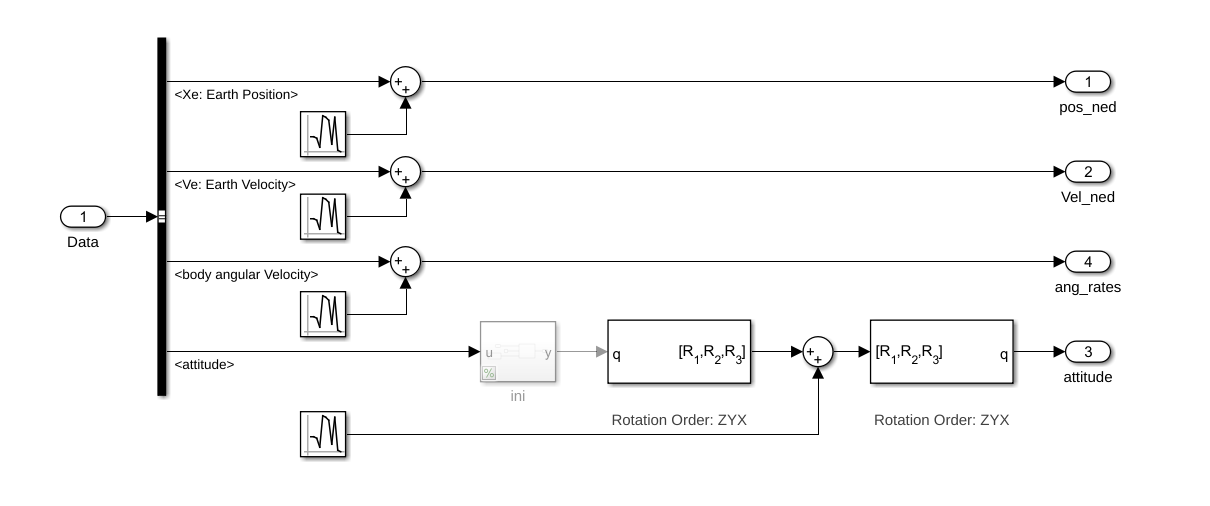
\includegraphics[width=0.95\linewidth]{Images/Current Status.png}
    \caption{Signal filter block}
    \label{fig:signal_filter_block}
\end{figure}

\subsection{Fixed-Wing Attitude Controller}
In this section, the attitude control system of the VTOL in the fixed-wing phase is presented in detail. The main structure is derived from \cite{px4controller}. Longitudinal and lateral dynamics are assumed to be uncoupled. The variables that have to be controlled are roll angle \( \phi \), pitch angle \( \theta \), and yaw rate \( \dot{\psi} \).

\subsubsection{Roll and Pitch Control}
The roll and pitch controllers follow a PID cascade loop structure (Figure \ref{fig:pid_cascade_loop}). The outer loop computes the error between the attitude setpoint \( \phi_{sp} \), \( \theta_{sp} \) and the estimated attitude \( \phi \), \( \theta \) respectively. This error, multiplied by the proportional gain \( P \), generates the Euler angle derivatives setpoint \( \dot{\phi}_{sp} \), \( \dot{\theta}_{sp} \), which is then converted into body rate setpoint \( p_{sp} \), \( q_{sp} \) with the matrix \( E \). The inner loop computes the rate error and utilizes proportional and integral controllers (PI) to produce the desired control surface deflections \( \delta_a \), \( \delta_e \) (aileron and elevator respectively).

The yaw controller generates its yaw rate setpoint using the turn coordination constraint to minimize lateral acceleration.

\begin{figure}[h]
    \centering
    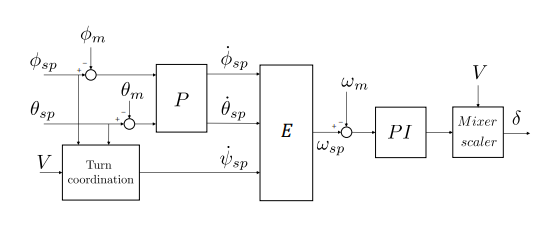
\includegraphics[width=1\linewidth]{Images/pid_cascade_loop.png}
    \caption{Fixed-wing Attitude Control Architecture: $\boldsymbol{\omega}$ is the body rates vector, $\boldsymbol{\delta}$ the control surfaces deflections vector ($\boldsymbol{\delta} = [\delta_a, \delta_e, \delta_r]$), and $V$ the airspeed.}
    \label{fig:pid_cascade_loop}
\end{figure}

\subsubsection{Yaw Rate Control: Turn Coordination}

During a turn maneuver (Figure \ref{fig:Forces during a turn}), the horizontal equilibrium yields:
\begin{equation}
    F_{\text{lift}} \sin \phi = mV \dot{\psi}
\end{equation}
where \( F_{\text{lift}} \) is the lift, \( V \) the aircraft speed, \( m \) the aircraft mass, and \( \dot{\psi} \) the yaw rate. The vertical component must balance gravity:
\begin{equation}
    F_{\text{lift}} \cos \phi = mg
\end{equation}
This leads to the yaw rate equation:
\begin{equation}
    \dot{\psi} = \frac{g}{V} \tan \phi \cos \theta
\end{equation}

A scaling factor \( K_{\text{scaler}} \) adjusts the control action based on airspeed \( V \), while saturation limits are applied to control surface deflections (Table \ref{tab:Maximum measured surfaces deflections.}).

\begin{figure}[h]
    \centering
    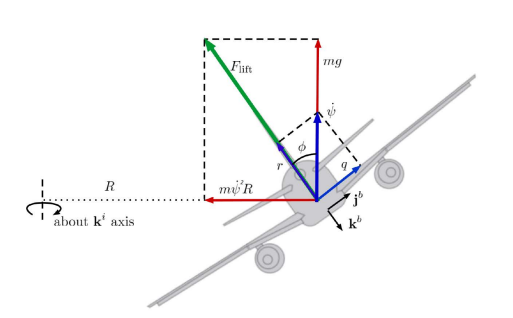
\includegraphics[width=0.9\linewidth]{Images/Forces during a turn, from [35].png}
    \caption{Forces during a turn}
    \label{fig:Forces during a turn}
\end{figure}

\begin{table}[h]
    \centering
    \begin{tabular}{ccc}
    \hline
        Rudder & Elevator & Aileron \\
    \hline
        \(50^\circ\) Left & \(60^\circ\) Down & \(35^\circ\) Down \\
        \(55^\circ\) Right & \(-50^\circ\) Up & \(-45^\circ\) Up \\
    \hline
    \end{tabular}
    \caption{Maximum measured surfaces deflections}
    \label{tab:Maximum measured surfaces deflections.}
\end{table}

\subsubsection{Total Energy Control System (TECS)}
In TECS (Total Energy Control System), managing both true airspeed and altitude simultaneously poses a challenge due to the coupled responses of the aircraft. Traditional Single-Input Single-Output (SISO) controllers handle each control variable separately, often leading to control coupling issues. TECS offers a solution by reframing the problem in terms of energies rather than original setpoints. By transforming initial setpoints into energy quantities, the control problem becomes decoupled. Thrust is then utilized to regulate the specific total energy of the aircraft, while pitch maintains a balance between potential and kinetic energy.

\subsubsection{Controller Algorithm}
The analysis presented here is derived from \cite{faleiro1999analysis}. The total energy of an aircraft is expressed as the sum of kinetic and potential energy, and its derivative leads to the total energy rate. Thrust setpoint is used for total energy control, while elevator is considered for energy distribution control. A simple control law, using proportional and integral control feedback, can be formulated. The control outputs are the normalized thrust and the pitch angle. Feedbacks of specific energy rate and energy balance rate are used to avoid the creation of unwanted zeros in the system transfer functions. The main structure of the algorithm is shown in Figure \ref{fig:TECS algorithm structure}.

\begin{figure}
    \centering
    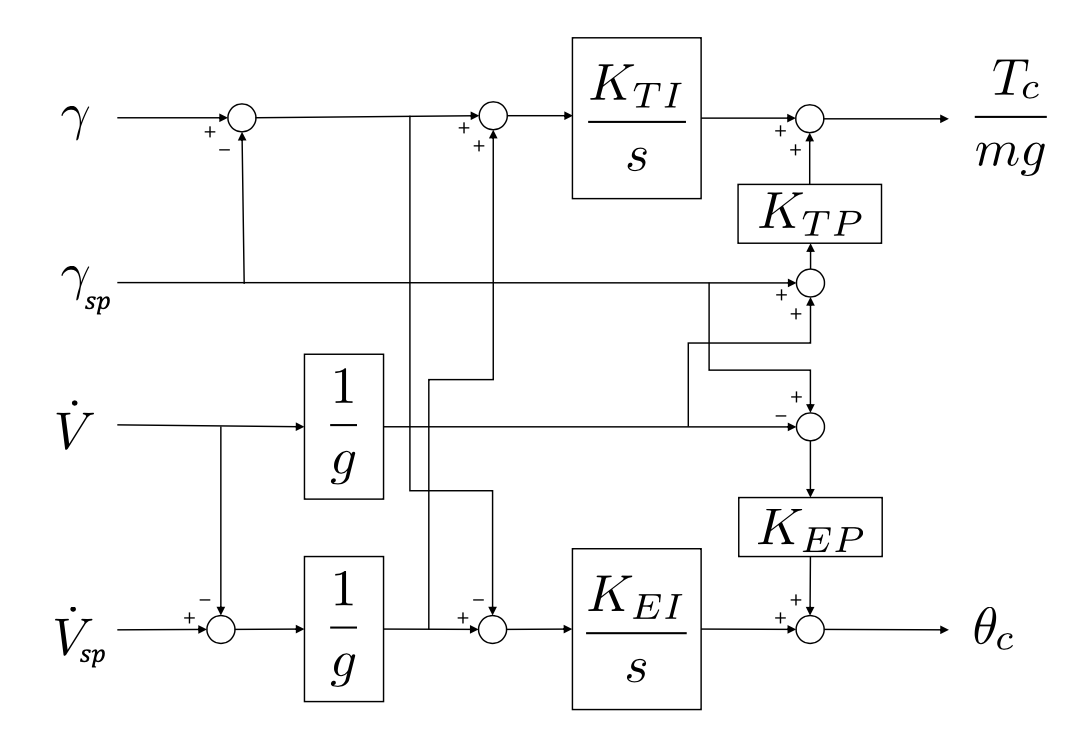
\includegraphics[width=0.9\linewidth]{Images/TECS algorithm structure..png}
    \caption{TECS algorithm structure.}
    \label{fig:TECS algorithm structure}
\end{figure}

\subsubsection{Controller Input and Output}
From a control perspective, the interest lies in altitude \( H_{sp} \) and speed \( V_{sp} \). The flight path angle \( \gamma_{sp} \) and the normalized longitudinal acceleration \( \frac{{\dot{V}_{sp}}}{{g}} \) are computed externally using a proportional controller on height and velocity error:
\begin{align}
    \dot{V}_{sp} &= K_v (V_{sp} - V), \\
    \dot{H}_{sp} &= K_H (H_{sp} - H), \\
    \gamma_{sp} &= \frac{{\dot{H}_{sp}}}{{V}}.
\end{align}
Speed and altitude errors are weighted equally to achieve decoupled control and efficient energy management during simultaneous flight path and speed maneuvers. Thus, the gains \( K_v \) and \( K_H \) should be equal \cite{faleiro1999analysis}.

These commands, \( \dot{V}_{sp} \) and \( \gamma_{sp} \), must be limited according to the aircraft performance to stay within a safe flight envelope.

For the input measurement \( \dot{V} \), it is suggested \cite{fari2017guidance} to take the acceleration measurement on the \( b_1 \) axis and subtract the contribution given by gravity:
\begin{equation}
    \dot{V} = a_x - g \sin \theta.
\end{equation}

The outputs of the TECS controller consist of a normalized thrust \( \frac{{T_c}}{{mg}} \) and a pitch angle \( \theta_c \). The latter is given as input into the attitude controller. Thus, the performance of TECS is directly affected by the performance of the pitch control loop.

The normalized thrust, after multiplication with the aircraft weight, is converted into throttle command \( \delta_t \) according to the following relations:
\begin{align}
    \Omega = \sqrt{\frac{{T_c}}{{K_T n_{\text{motors}}}}}
    \delta_t = \frac{{\Omega - q_{\text{fwd}}}}{{m_{\text{fwd}}}}
\end{align}
where \( \Omega \) is the angular speed of the motors. The coefficients \( K_T \), \( q_{\text{fwd}} \), and \( m_{\text{fwd}} \) have been computed in \cite{martello2021}.

\subsection{Optimization of the Throttle command generation block}
The original throttle command generation module operates under the assumption that the influence of incoming airflow can be neglected. However, this can lead to significant errors in estimating the thrust and torque generated by the propellers. To address this issue, a new Throttle Command Generation Module is developed, building upon the theoretical framework introduced in Section \ref{section:force elements} of Chapter \ref{ch:chapter1}. This new module utilizes equations (\ref{eq:thrust_1}) to (\ref{eq:outcome_airflow}) to predict the required motor angular velocity, thrusts, and torques based on this theory, thereby improving the accuracy of throttle commands.

Equation (\ref{eq:outcome_airflow}) requires knowledge of the motor's angular velocity and incoming airflow to calculate generated thrusts and torques. To ensure compatibility with real-world flight conditions, default throttle values are set for both fixed-wing and multi-copter modes. In fixed-wing mode, where the drone maintains a stable airspeed of $15 \text{ m/s}$, the throttle is set to $40\%$. Similarly, in multi-copter mode, where the drone is hovering, the assumed throttle value is set to $45\%$.

Additionally, due to the computational cost of the control system and the complexity of measuring incoming airflow for each propeller, a simplification in the calculation is necessary. Therefore, the incoming airflow is approximated by the body velocity of the drone itself. This simplification is justified by the negligible rotation speed of the drone compared to the cruise speed in fixed-wing mode and the climb/descent speed in multi-copter mode.

\begin{figure}
    \centering
    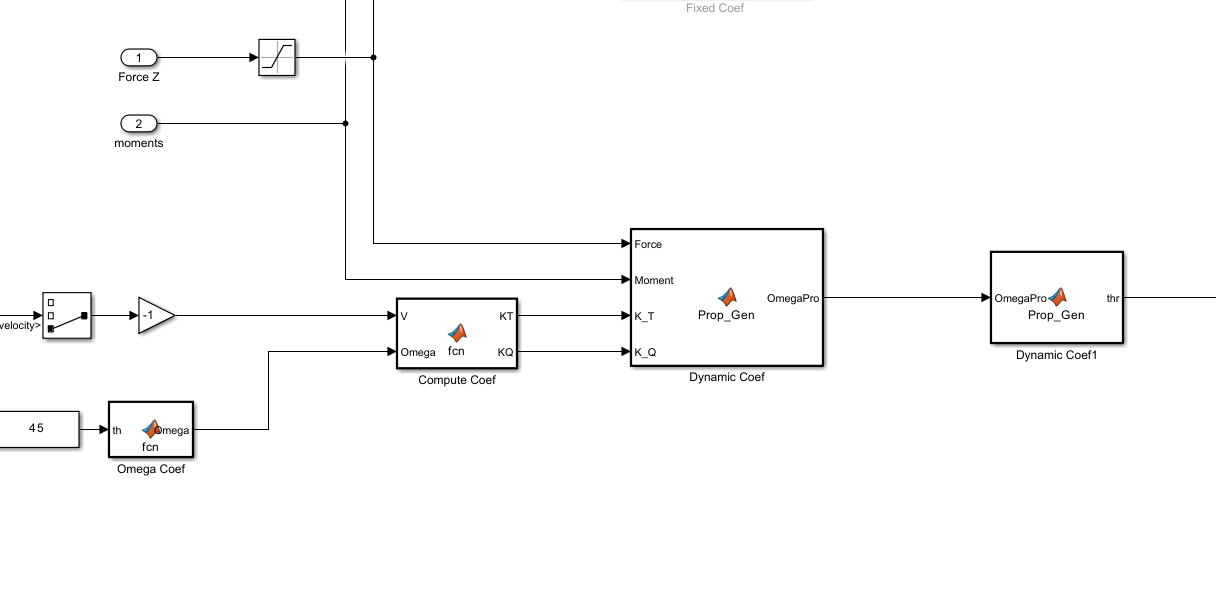
\includegraphics[width=0.9\linewidth]{Images/throttle command generation block.png}
    \caption{Throttle Command Generation Module.}
    \label{fig:Throttle Command Generation Module}
\end{figure}


\chapter{Maneuver Performance}

\section{Gust Wind}

Gust wind is a pivotal factor considered in evaluating aircraft handling qualities, as delineated in ADS-33 (Aeronautical Design Standard). A gust denotes a sudden and temporary increase in wind speed or alteration in wind direction experienced by an aircraft during flight. These gusts can arise from diverse atmospheric conditions, including thermal activity, weather fronts, or terrain features \cite{Wu2019}.

ADS-33 furnishes guidelines for assessing aircraft handling qualities in gusty conditions to ensure the aircraft remains controllable and predictable for the pilot. This standard delineates specific gust inputs applied to the aircraft during flight tests to evaluate its response and behavior.

These gust inputs typically involve step changes in airspeed and/or altitude, simulating the effects of encountering a gust \cite{raza2015autonomous}. Standardized to represent different levels of turbulence severity, these inputs are applied during specific flight maneuvers such as level flight, climbing, descending, or turning.

During flight testing pursuant to ADS-33, the aircraft's response to gust inputs is evaluated based on predetermined criteria related to stability, control authority, pilot workload, and aircraft behavior. The objective is to ensure the aircraft maintains stability and controllability under various gust conditions, enabling the pilot to conduct safe and effective flight operations.

Essentially, gust wind testing in ADS-33 aims to assess the aircraft's ability to withstand turbulent atmospheric conditions and provide a satisfactory level of handling qualities for the pilot, thereby enhancing flight safety and operational capability.

\subsection{Gust Wind Verification}

To accurately assess the impact of gust wind on an airframe, gusty wind is employed to analyze the effects of gust wind on force and moment in different orientations.

Using a clamp joint to secure the airframe on the ground and introducing a step signal to simulate moving gust wind, measurements of reaction force and moment on the clamp joint at the mass center position can be carefully observed.

This experimental setup involves a wind velocity of 1 m/s while the gust wind value is set at 10 m/s, with evaluations conducted in the x, y, and z axes. Figure \ref{fig:Gust} illustrates the case where gust in the Z-axis moves backward along the X-axis. To analyze the influence of gust wind on the propeller, two additional horizontal rotors are utilized with the throttle set at 50\% in case 1 and case 2, and vertical rotors are also utilized with the throttle set at 50\% in case 4. Using Equation \ref{eq:th2Omega}, the angular velocity of the rotor is calculated as:

\begin{equation}
    \Omega_{\text{thr50\%}} = 1579.8 \, \text{rad/s}
\end{equation}

The total verification case consists of 4 scenarios:

\begin{figure}[htbp]
    \centering
    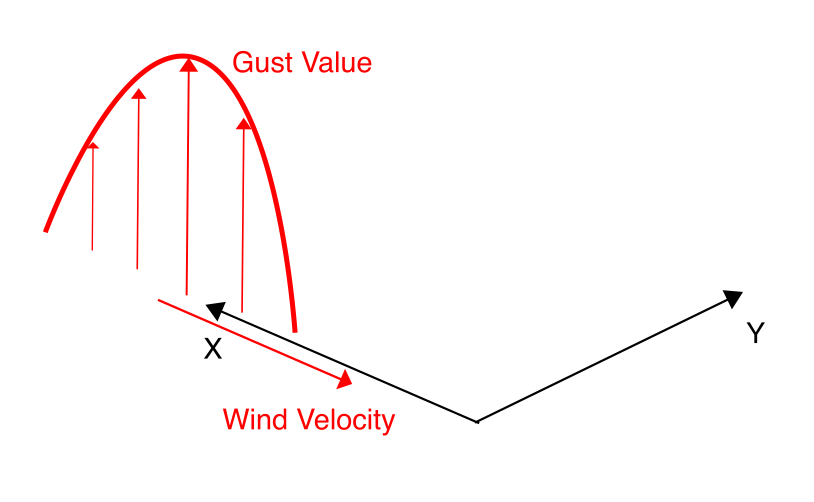
\includegraphics[width=0.85\linewidth]{Images/Gust.png}
    \caption{Gust Movement}
    \label{fig:Gust}
\end{figure}

\begin{itemize}
    \item Case 1: -10 m/s Gust in X-axis: Gust wind moves backward along the X-axis with 1 m/s.
    \item Case 2: 10 m/s Gust in X-axis: Gust wind moves forward along the X-axis with 1 m/s.
    \item Case 3: 10 m/s Gust in Y-axis: Gust wind moves forward along the Y-axis with 1 m/s.
    \item Case 4: 10 m/s Gust in Z-axis: Gust wind moves backward along the X-axis with 1 m/s.
\end{itemize}

Figures \ref{fig:fixed -x}, \ref{fig:fixed x}, \ref{fig:fixed y}, and \ref{fig:fixed z} depict the change of reaction force and moment of the joint at the mass center.

In Chapter \ref{ch:chapter1}, Section \ref{section:Aerodynamic elements}, aerodynamic force and moment generated by the wing are introduced, and in Section \ref{section:force elements}, the thrust force generated by the propeller is introduced by Equation \ref{eq:thrust}. Based on these equations, reaction force and moment acting on the clamp joint can be analyzed.

\begin{figure}[htbp]
    \centering
    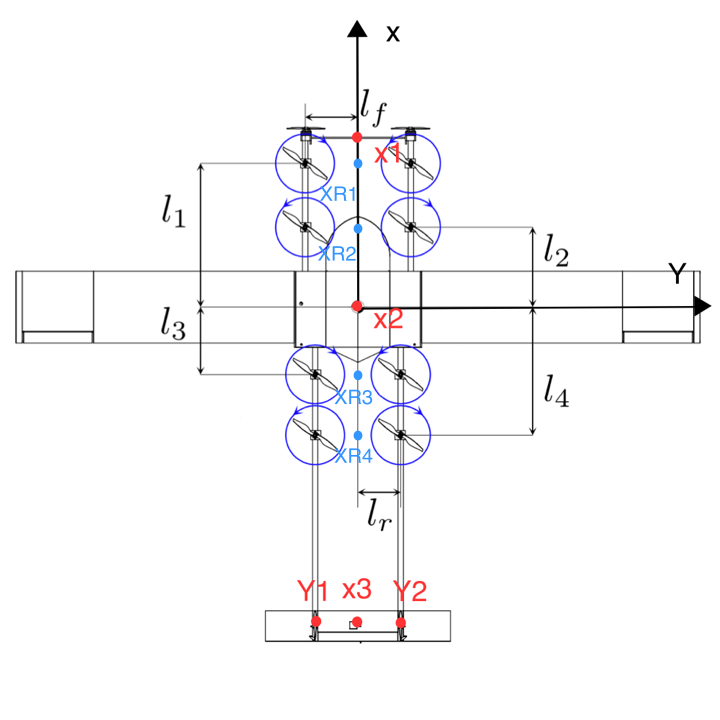
\includegraphics[width=0.75\linewidth]{Images/Gust_Position.png}
    \caption{Gust Position}
    \label{fig:Gust position}
\end{figure}

\textbf{Case 1:} In Figure \ref{fig:fixed -x}, as depicted in Figure \ref{fig:Gust position}, the gust moves backward along the X-axis. When the gust arrives at different positions, the force and moment change. When the gust passes through position \textit{X1}, the thrust force generated by the propeller decreases due to gust airflow. Then, when the gust arrives at position \textit{X2}, the main wing generates a large lift and drag due to the gust. Finally, when the gust arrives at position \textit{X3}, the tail wing generates lift and drag. Due to the smaller pitch angle and wing surface compared to the main wing, the effect on the reaction force and moment changes less. The values are summarized in Table \ref{tab:verify -x}.

\textbf{Case 2:} Similarly, in Figure \ref{fig:fixed x}, the gust moves forward along the X-axis. The gust would arrive at position \textit{X3} first, then arrive at position \textit{X2}. The computed values are summarized in Table \ref{tab:verify x}.

\textbf{Case 3:} In Figure \ref{fig:fixed y}, the reaction force and moment are generated due to the vertical tail wing. The gust moves forward along the Y-axis, arriving at position \textit{Y1} first, then position \textit{Y2}. The computed values are summarized in Table \ref{tab:verify y}.

\textbf{Case 4:} In Figure \ref{fig:fixed z}, the gust moves backward along the X-axis, which is Similar with case 1, when the gust arrives at position \textit{X2}, the main wing generates a large lift and drag due to the gust, and when the gust arrives at position \textit{X3}. When the gust passes through position of each vertical propeller, the thrust force generated by the propeller increase in turn due to gust airflow. The computed values are summarized in Table \ref{tab:verify z}.

Comparing the computed values and measured values in simulation, due to an error between hand-computed and simulation values below $1 \times 10^{-6}$, they can be considered equivalent.

\begin{table}
    \centering
    \begin{tabular}{ccccc}
    \hline
        Position & Time Delay (s) & $F_{X}$ (N) & $F_{Z}$ (N) & $M_{Y}$ (N*m) \\
    \hline
        before X1   &       & 5.1002 & 0        & 0 \\
        X1          &       & 2.0135 & 0        & 0 \\
        X2          & 0.4960 & 1.0533 & -24.8717 & 0.899845 \\
        X3          & 1.08  & 0.9507 & -25.6849  & 0.0801132\\
    \hline
    \end{tabular}
    \caption{Joint reaction force, moment change and time delay when gust move backward along X-axis}
    \label{tab:verify -x}
\end{table}

\begin{table}
    \centering
    \begin{tabular}{ccccc}
    \hline
        Position & Time Delay (s) & $F_{X}$ (N) & $F_{Z}$ (N) & $M_{Y}$ (N*m) \\
    \hline
        before X3   &       & 5.1004 & 0        & 0 \\
        X3          &       & 5.31  & 1.09691 & 1.15002 \\
        X2          & 1.08  & 7.17  & 15.4294 & 1.5691 \\
        X1          & 0.4960 & 9.16 & 15.4294 & 1.5691 \\
    \hline
    \end{tabular}
    \caption{Joint reaction force, moment change and time delay change when gust move forward along X-axis}
    \label{tab:verify x}
\end{table}

\begin{table}
    \centering
    \begin{tabular}{cccccc}
    \hline
        Position & Time Delay (s) & $F_{X}$ (N) & $F_{Y}$ (N)& $M_{X}$ (N*m) & $M_{Z}$ (N*m) \\
    \hline
        before Y1   &           & 5.1004 & 0        & 0         & 0 \\
        Y1          &           & 5.1689 & -2.20449 & -0.1962   & 2.28083 \\
        Y2          & 0.2630    & 5.2368 & -4.40897 & -0.392398 & 4.57972 \\
    \hline
    \end{tabular}
    \caption{Joint reaction force, moment change and time delay when gust move forward along Y-axis}
    \label{tab:verify y}
\end{table}
% REDONE
\begin{table}
    \centering
    \begin{tabular}{ccccc}
    \hline
        Position & Time Delay (s) & $F_{X}$ (N) & $F_{Z}$ (N) & $M_{Y}$ (N*m)\\
    \hline
        before XR1  &       &  0        & -65.68    & 2.34        \\       
        XR1         &       &  0        & -69.45    & 3.91         \\   
        XR2         & 0.146 &  0        & -73.22   & 4.92        \\       
        X2          & 0.267 &  -1.593   & -142.889  & 5.2433     \\       
        XR3         & 0.191 &  -1.593   & -146.664   & 4.4889      \\       
        XR4         & 0.146 &  -1.593   & -150.439  &  3.195    \\           
        X3          & 0.67  &  -1.66    & -157.54   &  -4.185    \\           
    \hline
    \end{tabular}
    \caption{Joint reaction force, moment change and time delay when gust move forward along Z-axis}
    \label{tab:verify z}
\end{table}

\begin{figure}[htbp]
  \centering
  \begin{minipage}[b]{0.3\textwidth}
    \centering
    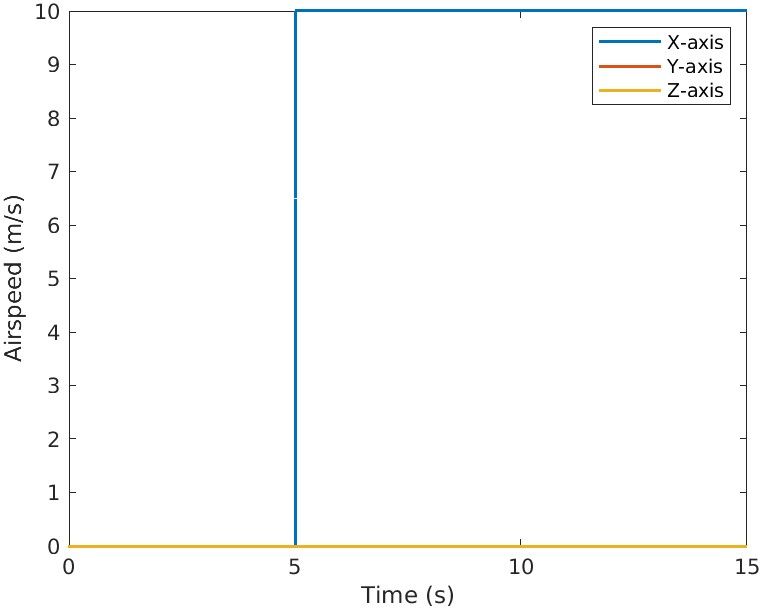
\includegraphics[width=\textwidth]{Images/Gust/FIXED/1 airspeed_1.jpg}
    \caption*{\textit{True Airspeed}}
  \end{minipage}
  \hfil
  \begin{minipage}[b]{0.3\textwidth}
    \centering
    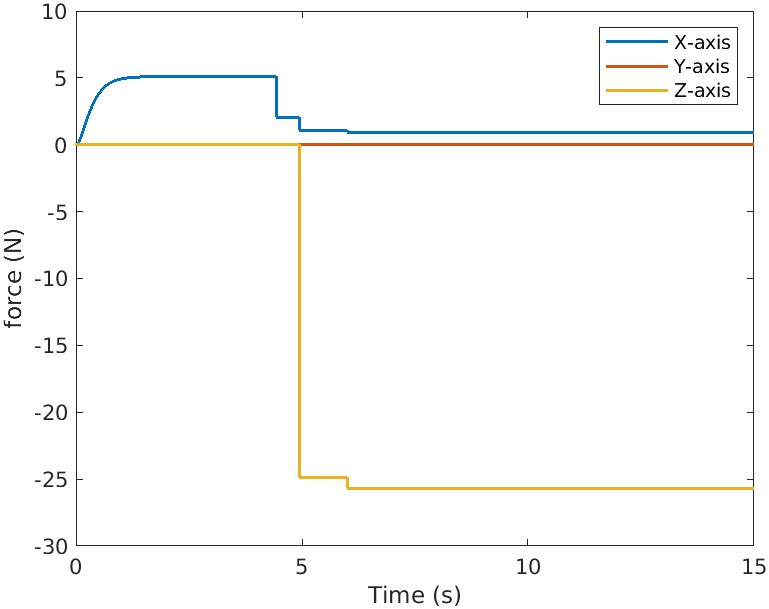
\includegraphics[width=\textwidth]{Images/Gust/FIXED/2 force_1.jpg}
    \caption*{\textit{Reaction Force}}
  \end{minipage}
  \hfil
  \begin{minipage}[b]{0.3\textwidth}
    \centering
    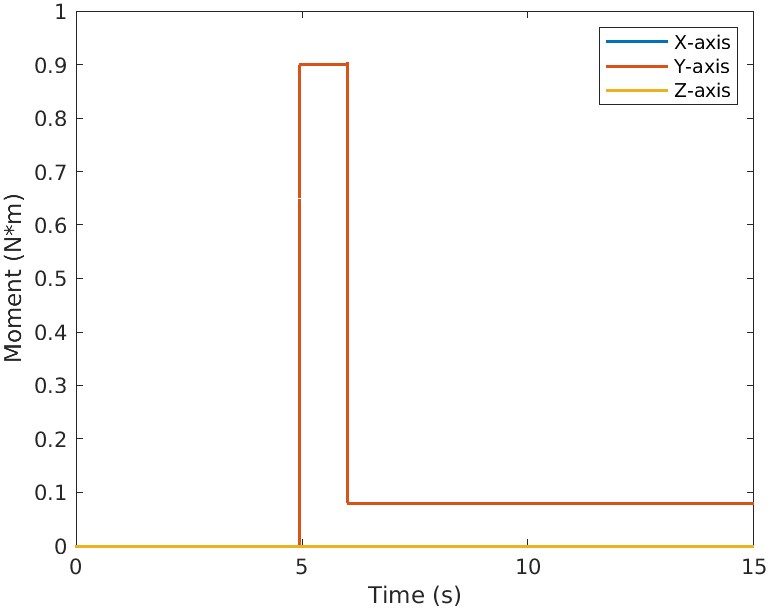
\includegraphics[width=\textwidth]{Images/Gust/FIXED/3 moment_1.jpg}
    \caption*{\textit{Reaction Moment}}
  \end{minipage}
  \caption{Status in mass center of airframe when step gust move backward along X-axis}
  \label{fig:fixed -x}
\end{figure}

\begin{figure}[htbp]
  \centering
  \begin{minipage}[b]{0.3\textwidth}
    \centering
    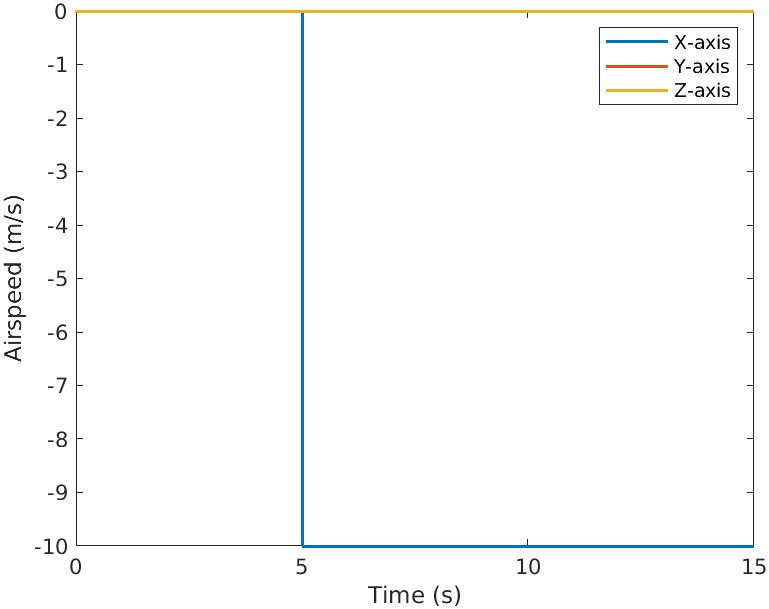
\includegraphics[width=\textwidth]{Images/Gust/FIXED/1 airspeed_2.jpg}
    \caption*{\textit{True Airspeed}}
  \end{minipage}
  \hfil
  \begin{minipage}[b]{0.3\textwidth}
    \centering
    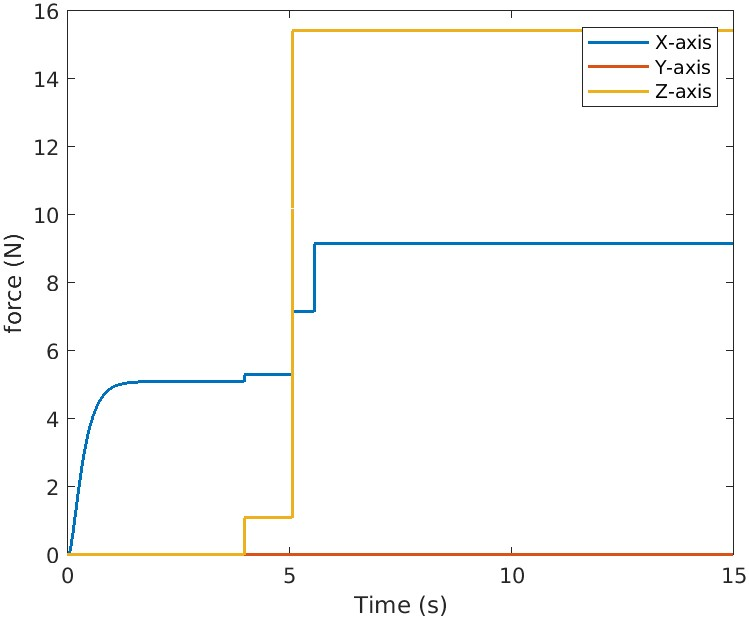
\includegraphics[width=\textwidth]{Images/Gust/FIXED/2 force_2.jpg}
    \caption*{\textit{Reaction Force}}
  \end{minipage}
  \hfil
  \begin{minipage}[b]{0.3\textwidth}
    \centering
    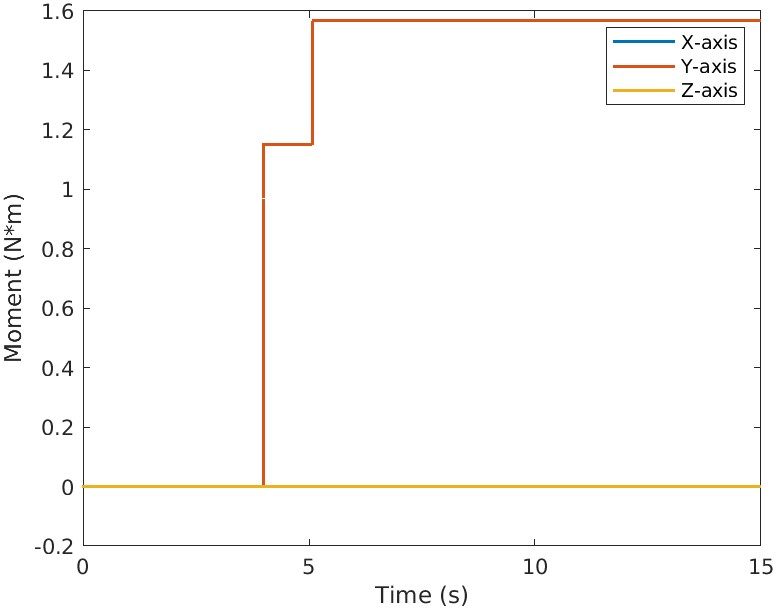
\includegraphics[width=\textwidth]{Images/Gust/FIXED/3 moment_2.jpg}
    \caption*{\textit{Reaction Moment}}
  \end{minipage}
  \caption{Status in mass center of airframe when step gust move forward along X-axis}
  \label{fig:fixed x}
\end{figure}

\begin{figure}[htbp]
  \centering
  \begin{minipage}[b]{0.3\textwidth}
    \centering
    \includegraphics[width=\textwidth]{Images/Gust/FIXED/1 airspeed_3.jpg}
    \caption*{\textit{True Airspeed}}
  \end{minipage}
  \hfil
  \begin{minipage}[b]{0.3\textwidth}
    \centering
    \includegraphics[width=\textwidth]{Images/Gust/FIXED/2 force_3.jpg}
    \caption*{\textit{Reaction Force}}
  \end{minipage}
  \hfil
  \begin{minipage}[b]{0.3\textwidth}
    \centering
    \includegraphics[width=\textwidth]{Images/Gust/FIXED/3 moment_3.jpg}
    \caption*{\textit{Reaction Moment}}
  \end{minipage}
  \caption{Status in mass center of airframe when step gust move forward along Y-axis}
  \label{fig:fixed y}
\end{figure}
% REDONE
\begin{figure}[htbp]
  \centering
  \begin{minipage}[b]{0.3\textwidth}
    \centering
    \includegraphics[width=\textwidth]{Images/Gust/FIXED/1 airspeed_4.jpg}
    \caption*{\textit{True Airspeed}}
  \end{minipage}
  \hfil
  \begin{minipage}[b]{0.3\textwidth}
    \centering
    \includegraphics[width=\textwidth]{Images/Gust/FIXED/2 force_4.jpg}
    \caption*{\textit{Reaction Force}}
  \end{minipage}
  \hfil
  \begin{minipage}[b]{0.3\textwidth}
    \centering
    \includegraphics[width=\textwidth]{Images/Gust/FIXED/3 moment_4.jpg}
    \caption*{\textit{Reaction Moment}}
  \end{minipage}
  \caption{Status in mass center of airframe when step gust move forward along Z-axis}
  \label{fig:fixed z}
\end{figure}

\subsection{Gust Experimental Test Procedure and Setup}

When comparing this specific UAV to traditional helicopters and multi-copter UAVs, it is essential to consider its additional wing structure, which can significantly influence its performance in gusty winds. According to ADS-33 regulations, the drone undergoes gust testing under various wind conditions, ranging from calm (0-5 knots, 0-2.57 m/s), light (10-15 knot, 5.14-7.72 m/s)  moderate (25-35 knots, 12.86-18.01 m/s). While most missions can be accomplished in calm or light winds, the drone is specifically scrutinized for its performance in gusts across all three axes, Since the unit of wind speed in ADS-33E is knots, the unit of wind speed in this section is still knots.

In the \textit{Air properties} element of MBDyn, various gust wind models are available for selection. The Front 1D type stands out as the most suitable model for simulating gusts in a realistic environment. To accurately replicate real-world conditions during drone flights, the cosine function is employed to depict the behavior of gusts. Gusty winds for drones predominantly manifest in two forms: pulse gusty winds and constant gusty winds. For pulse gusts, a single cycle lasting 5 seconds is utilized, while a half cycle is employed for step gusts to transition the gust value from 0 knots to the desired gust value. This meticulous approach ensures the precision and reliability of our simulations. Gust wind is programmed to reach the original center of the global frame precisely 5 seconds into the simulation when the drone operates in multi-copter mode and remains in hover status.

During multi-copter mode operations, the control system is configured to focus solely on gust resistance testing, as this particular test case primarily evaluates the aircraft's ability to withstand gusts. Therefore, position hold control can be disregarded. In gust testing, multi-copter mode exclusively employs velocity control after climbing to required altitude, with all velocity setpoints set to null. Additionally, yaw angle control is set to null to maintain the aircraft's heading direction. The total experimental test cases for gust resistance are summarized in Table \ref{tab:gust VTOL}.

\begin{sidewaystable}[htbp]
    \centering
    \begin{tabular}{ccccc}
    \hline
        Control Mode & Gust Type & Gust Direction & Gust Value (knots) & Move Direction \\
        \hline
        multicopter Mode & Step & X-axis & -35 & Backward along X-axis \\
        multicopter Mode & Step & X-axis & 10 & Forward along X-axis \\
        multicopter Mode & Step & Y-axis & 5 & Forward along Y-axis \\
        multicopter Mode & Step & Y-axis & 5 & Backward along X-axis \\
        multicopter Mode & Step & Z-axis & 15 & Backward along X-axis \\
        \hline
        multicopter Mode & Pulse & X-axis & -35 & Forward along X-axis \\
        multicopter Mode & Pulse & X-axis & 20 & Backward along X-axis \\
        multicopter Mode & Pulse & Y-axis & 5 & Forward along Y-axis \\
        multicopter Mode & Pulse & Y-axis & 5 & Backward along X-axis \\
        multicopter Mode & Pulse & Z-axis & 15 & Backward along X-axis \\
        \hline
        Fixed-wing Mode & Pulse & X-axis & -15 & Backward along X-axis \\
        Fixed-wing Mode & Pulse & X-axis & -5 & forward along X-axis \\
        Fixed-wing Mode & Pulse & Y-axis & 15 & Backward along X-axis \\
        Fixed-wing Mode & Pulse & Z-axis & 15 & Backward along X-axis \\
    \hline
    \end{tabular}
    \caption{Gust Test of Aircraft in Multicopter Mode}
    \label{tab:gust VTOL}
\end{sidewaystable}

\subsubsection{Step Gust Test for Aircraft in Multi-Copter Mode}

The drone's response to a gust of wind moving along the X-axis from positive to negative directions illustrates in Figure \ref{fig:VTOL step -x} . This gust induces additional drag and lift on the drone's wing, resulting in a slight increase in altitude and backward movement. The drone exhibits resilience against moderate wind gusts under these conditions.

Conversely, in Figure \ref{fig:VTOL step x}, when a gust of wind moves forward along the X-axis, instability in the yaw angle, coupled with the effects of rolling and pitch angles, may cause the drone to lose control. The maximum tolerable gust under this circumstance is 10 knots.

Gusts along the Y-axis, depicted in Figures \ref{fig:VTOL step yy} and \ref{fig:VTOL step xy}, exert significant torque on the vertical tail wing, resulting in substantial yaw angle changes. However, the torque generated by the vertical propeller is limited, rendering the drone unable to withstand high gusts exceeding 5 knots.

Figure \ref{fig:VTOL step z} portrays the impact of gusts along the Z-axis. The main wing and horizontal tail experience elevated drag and lift, necessitating significant pitch angle adjustments to maintain force and moment distribution. Excessive gusts can induce large pitch angle changes, potentially resulting in loss of control. The maximum tolerable gust along the Z-axis is 15 knots.

In conclusion, while the aircraft demonstrates good resistance performance against gusts in the X-axis and Z-axis, its resistance capability is comparatively lower when gusts occur along the Y-axis, primarily due to the structural characteristics of the vertical tail wing.

\begin{figure}[htbp]
  \centering
  \begin{minipage}[b]{0.45\textwidth}
    \centering
    \includegraphics[width=\textwidth]{Images/Gust/VTOL step/1 position_1.jpg}
    \caption*{\textit{Position}}
  \end{minipage}
  \hfil
  \begin{minipage}[b]{0.45\textwidth}
    \centering
    \includegraphics[width=\textwidth]{Images/Gust/VTOL step/2 airspeed_1.jpg}
    \caption*{\textit{True Airspeed}}
  \end{minipage}
  \begin{minipage}[b]{0.45\textwidth}
    \centering
    \includegraphics[width=\textwidth]{Images/Gust/VTOL step/3 groundspeed_1.jpg}
    \caption*{\textit{Ground Speed}}
  \end{minipage}
  \hfil
  \begin{minipage}[b]{0.45\textwidth}
    \centering
    \includegraphics[width=\textwidth]{Images/Gust/VTOL step/4 EulerAngle_1.jpg}
    \caption*{\textit{Euler Angle}}
  \end{minipage}
  \caption{Status of aircraft in multicopter mode when step gust in negative X-axis move backward along X-axis}
  \label{fig:VTOL step -x}
\end{figure}

\begin{figure}[htbp]
  \centering
  \begin{minipage}[b]{0.45\textwidth}
    \centering
    \includegraphics[width=\textwidth]{Images/Gust/VTOL step/1 position_2.jpg}
    \caption*{\textit{Position}}
  \end{minipage}
  \hfil
  \begin{minipage}[b]{0.45\textwidth}
    \centering
    \includegraphics[width=\textwidth]{Images/Gust/VTOL step/2 airspeed_2.jpg}
    \caption*{\textit{True Airspeed}}
  \end{minipage}
  \begin{minipage}[b]{0.45\textwidth}
    \centering
    \includegraphics[width=\textwidth]{Images/Gust/VTOL step/3 groundspeed_2.jpg}
    \caption*{\textit{Ground Speed}}
  \end{minipage}
  \hfil
  \begin{minipage}[b]{0.45\textwidth}
    \centering
    \includegraphics[width=\textwidth]{Images/Gust/VTOL step/4 EulerAngle_2.jpg}
    \caption*{\textit{Euler Angle}}
  \end{minipage}
  \caption{Status of aircraft in multicopter mode when step gust in positive X-axis move forward along X-axis}
  \label{fig:VTOL step x}
\end{figure}

\begin{figure}[htbp]
  \centering
  \begin{minipage}[b]{0.45\textwidth}
    \centering
    \includegraphics[width=\textwidth]{Images/Gust/VTOL step/1 position_3.jpg}
    \caption*{\textit{Position}}
  \end{minipage}
  \hfil
  \begin{minipage}[b]{0.45\textwidth}
    \centering
    \includegraphics[width=\textwidth]{Images/Gust/VTOL step/2 airspeed_3.jpg}
    \caption*{\textit{True Airspeed}}
  \end{minipage}
  \begin{minipage}[b]{0.45\textwidth}
    \centering
    \includegraphics[width=\textwidth]{Images/Gust/VTOL step/3 groundspeed_3.jpg}
    \caption*{\textit{Ground Speed}}
  \end{minipage}
  \hfil
  \begin{minipage}[b]{0.45\textwidth}
    \centering
    \includegraphics[width=\textwidth]{Images/Gust/VTOL step/4 EulerAngle_3.jpg}
    \caption*{\textit{Euler Angle}}
  \end{minipage}
  \caption{Status of aircraft in multicopter mode when step gust in Y-axis move backward along X-axis}
  \label{fig:VTOL step xy}
\end{figure}

\begin{figure}[htbp]
  \centering
  \begin{minipage}[b]{0.45\textwidth}
    \centering
    \includegraphics[width=\textwidth]{Images/Gust/VTOL step/1 position_4.jpg}
    \caption*{\textit{Position}}
  \end{minipage}
  \hfil
  \begin{minipage}[b]{0.45\textwidth}
    \centering
    \includegraphics[width=\textwidth]{Images/Gust/VTOL step/2 airspeed_4.jpg}
    \caption*{\textit{True Airspeed}}
  \end{minipage}
  \begin{minipage}[b]{0.45\textwidth}
    \centering
    \includegraphics[width=\textwidth]{Images/Gust/VTOL step/3 groundspeed_4.jpg}
    \caption*{\textit{Ground Speed}}
  \end{minipage}
  \hfil
  \begin{minipage}[b]{0.45\textwidth}
    \centering
    \includegraphics[width=\textwidth]{Images/Gust/VTOL step/4 EulerAngle_4.jpg}
    \caption*{\textit{Euler Angle}}
  \end{minipage}
  \caption{Status of aircraft in multicopter mode when step gust in Z-axis move backward along X-axis}
  \label{fig:VTOL step z}
\end{figure}

\begin{figure}[htbp]
  \centering
  \begin{minipage}[b]{0.45\textwidth}
    \centering
    \includegraphics[width=\textwidth]{Images/Gust/VTOL step/1 position_5.jpg}
    \caption*{\textit{Position}}
  \end{minipage}
  \hfil
  \begin{minipage}[b]{0.45\textwidth}
    \centering
    \includegraphics[width=\textwidth]{Images/Gust/VTOL step/2 airspeed_5.jpg}
    \caption*{\textit{True Airspeed}}
  \end{minipage}
  \begin{minipage}[b]{0.45\textwidth}
    \centering
    \includegraphics[width=\textwidth]{Images/Gust/VTOL step/3 groundspeed_5.jpg}
    \caption*{\textit{Ground Speed}}
  \end{minipage}
  \hfil
  \begin{minipage}[b]{0.45\textwidth}
    \centering
    \includegraphics[width=\textwidth]{Images/Gust/VTOL step/4 EulerAngle_5.jpg}
    \caption*{\textit{Euler Angle}}
  \end{minipage}
  \caption{Status of aircraft in multicopter mode when step gust in Y-axis move forward along Y-axis}
  \label{fig:VTOL step yy}
\end{figure}

\subsubsection{Pulse Gust Test for Aircraft in Multi-Copter Mode}

The simulation results for the pulse gust case are comparable to those of the step gust case. Following the occurrence of the gust, the aircraft quickly recovers to a stable hover status. Notably, due to the nature of pulse gusts, aircraft in some instances (as depicted in Figure \ref{fig:VTOL pulse x}) exhibit the ability to withstand larger gusts before experiencing unstable attitudes compared to constant step gusts.

\begin{figure}[htbp]
  \centering
  \begin{minipage}[b]{0.45\textwidth}
    \centering
    \includegraphics[width=\textwidth]{Images/Gust/VTOL pulse/1 position_1.jpg}
    \caption*{\textit{Position}}
  \end{minipage}
  \hfil
  \begin{minipage}[b]{0.45\textwidth}
    \centering
    \includegraphics[width=\textwidth]{Images/Gust/VTOL pulse/2 airspeed_1.jpg}
    \caption*{\textit{True Airspeed}}
  \end{minipage}
  \begin{minipage}[b]{0.45\textwidth}
    \centering
    \includegraphics[width=\textwidth]{Images/Gust/VTOL pulse/3 groundspeed_1.jpg}
    \caption*{\textit{Ground Speed}}
  \end{minipage}
  \hfil
  \begin{minipage}[b]{0.45\textwidth}
    \centering
    \includegraphics[width=\textwidth]{Images/Gust/VTOL pulse/4 EulerAngle_1.jpg}
    \caption*{\textit{Euler Angle}}
  \end{minipage}
  \caption{Status of aircraft in multicopter mode when pulse gust in negative X-axis move backward along X-axis}
  \label{fig:VTOL pulse -x}
\end{figure}

\begin{figure}[htbp]
  \centering
  \begin{minipage}[b]{0.45\textwidth}
    \centering
    \includegraphics[width=\textwidth]{Images/Gust/VTOL pulse/1 position_2.jpg}
    \caption*{\textit{Position}}
  \end{minipage}
  \hfil
  \begin{minipage}[b]{0.45\textwidth}
    \centering
    \includegraphics[width=\textwidth]{Images/Gust/VTOL pulse/2 airspeed_2.jpg}
    \caption*{\textit{True Airspeed}}
  \end{minipage}
  \begin{minipage}[b]{0.45\textwidth}
    \centering
    \includegraphics[width=\textwidth]{Images/Gust/VTOL pulse/3 groundspeed_2.jpg}
    \caption*{\textit{Ground Speed}}
  \end{minipage}
  \hfil
  \begin{minipage}[b]{0.45\textwidth}
    \centering
    \includegraphics[width=\textwidth]{Images/Gust/VTOL pulse/4 EulerAngle_2.jpg}
    \caption*{\textit{Euler Angle}}
  \end{minipage}
  \caption{Status of aircraft in multicopter mode when pulse gust in positive X-axis move forward along X-axis}
  \label{fig:VTOL pulse x}
\end{figure}

\begin{figure}[htbp]
  \centering
  \begin{minipage}[b]{0.45\textwidth}
    \centering
    \includegraphics[width=\textwidth]{Images/Gust/VTOL pulse/1 position_3.jpg}
    \caption*{\textit{Position}}
  \end{minipage}
  \hfil
  \begin{minipage}[b]{0.45\textwidth}
    \centering
    \includegraphics[width=\textwidth]{Images/Gust/VTOL pulse/2 airspeed_3.jpg}
    \caption*{\textit{True Airspeed}}
  \end{minipage}
  \begin{minipage}[b]{0.45\textwidth}
    \centering
    \includegraphics[width=\textwidth]{Images/Gust/VTOL pulse/3 groundspeed_3.jpg}
    \caption*{\textit{Ground Speed}}
  \end{minipage}
  \hfil
  \begin{minipage}[b]{0.45\textwidth}
    \centering
    \includegraphics[width=\textwidth]{Images/Gust/VTOL pulse/4 EulerAngle_3.jpg}
    \caption*{\textit{Euler Angle}}
  \end{minipage}
  \caption{Status in aircraft in multicopter mode when pulse gust in Y-axis move backward along X-axis}
  \label{fig:VTOL pulse xy}
\end{figure}

\begin{figure}[htbp]
  \centering
  \begin{minipage}[b]{0.45\textwidth}
    \centering
    \includegraphics[width=\textwidth]{Images/Gust/VTOL pulse/1 position_4.jpg}
    \caption*{\textit{Position}}
  \end{minipage}
  \hfil
  \begin{minipage}[b]{0.45\textwidth}
    \centering
    \includegraphics[width=\textwidth]{Images/Gust/VTOL pulse/2 airspeed_4.jpg}
    \caption*{\textit{True Airspeed}}
  \end{minipage}
  \begin{minipage}[b]{0.45\textwidth}
    \centering
    \includegraphics[width=\textwidth]{Images/Gust/VTOL pulse/3 groundspeed_4.jpg}
    \caption*{\textit{Ground Speed}}
  \end{minipage}
  \hfil
  \begin{minipage}[b]{0.45\textwidth}
    \centering
    \includegraphics[width=\textwidth]{Images/Gust/VTOL pulse/4 EulerAngle_4.jpg}
    \caption*{\textit{Euler Angle}}
  \end{minipage}
  \caption{Status of aircraft in multicopter mode when pulse gust in Z-axis move backward along X-axis}
  \label{fig:VTOL pulse z}
\end{figure}

\begin{figure}[htbp]
  \centering
  \begin{minipage}[b]{0.45\textwidth}
    \centering
    \includegraphics[width=\textwidth]{Images/Gust/VTOL pulse/1 position_5.jpg}
    \caption*{\textit{Position}}
  \end{minipage}
  \hfil
  \begin{minipage}[b]{0.45\textwidth}
    \centering
    \includegraphics[width=\textwidth]{Images/Gust/VTOL pulse/2 airspeed_5.jpg}
    \caption*{\textit{True Airspeed}}
  \end{minipage}
  \begin{minipage}[b]{0.45\textwidth}
    \centering
    \includegraphics[width=\textwidth]{Images/Gust/VTOL pulse/3 groundspeed_5.jpg}
    \caption*{\textit{Ground Speed}}
  \end{minipage}
  \hfil
  \begin{minipage}[b]{0.45\textwidth}
    \centering
    \includegraphics[width=\textwidth]{Images/Gust/VTOL pulse/4 EulerAngle_5.jpg}
    \caption*{\textit{Euler Angle}}
  \end{minipage}
  \caption{Status of aircraft in multicopter mode when pulse gust in Y-axis move forward along Y-axis}
  \label{fig:VTOL pulse yy}
\end{figure}

\subsubsection{Pulse Gust Test in Forward Flight Mode}

During the Pulse Gust Test in forward flight mode, the control system transitions to fixed-wing mode, maintaining constant $v_{\text{cruise}}$ and altitude. Yaw and roll angle control are set to null.

The incorporation of an additional saturation module into the pitch setpoint input of the $TECS_m$ control system facilitated the examination of pulse gusty wind effects in forward flight mode. Unlike step gusts, which are unrealistic in forward flight mode, only pulse gusty winds were considered. Key observations from these conditions are detailed below:

At approximately 10 seconds into the simulation, the drone encountered a pulse gust of wind. Due to the concurrent movement of the aircraft and gusty wind along the X-axis, precise synchronization between the gust and the drone's position was unattainable. Consequently, the aircraft could only withstand gusts of up to 5 knots from the X direction without compromising its stability. In other scenarios, the aircraft demonstrated resilience against pulse gusts of up to 15 knots.

In Figure \ref{fig:Gust FWD pulse y}, the simulation results indicate an additional yaw angle generated after a gust in the Y-axis occurs, causing the aircraft to deviate from its original course.

When subjected to a pulse gust along the Z-axis, control complexity increased due to changes in altitude and airspeed. Figure \ref{fig:Gust FWD pulse z} illustrates the response of the $TECS_m$ system, tasked with maintaining airspeed while controlling altitude to return to the designated altitude. This simultaneous adjustment of throttle and movable surfaces introduced delays, particularly evident in altitude control due to the high value of the integration factor in the $TECS_m$ system. Consequently, the total control system required additional time to stabilize the aircraft.

\begin{figure}[htbp]
  \centering
  \begin{minipage}[b]{0.45\textwidth}
    \centering
    \includegraphics[width=\textwidth]{Images/Gust/Gust FWD pulse 0428/1 position_1.jpg}
    \caption*{\textit{Position}}
  \end{minipage}
  \hfil
  \begin{minipage}[b]{0.45\textwidth}
    \centering
    \includegraphics[width=\textwidth]{Images/Gust/Gust FWD pulse 0428/2 TAS_1.jpg}
    \caption*{\textit{Airspeed in global frame}}
  \end{minipage}
  \begin{minipage}[b]{0.45\textwidth}
    \centering
    \includegraphics[width=\textwidth]{Images/Gust/Gust FWD pulse 0428/3 groundspeed_1.jpg}
    \caption*{\textit{Ground Speed}}
  \end{minipage}
  \hfil
  \begin{minipage}[b]{0.45\textwidth}
    \centering
    \includegraphics[width=\textwidth]{Images/Gust/Gust FWD pulse 0428/4 EulerAngle_1.jpg}
    \caption*{\textit{Euler Angle}}
  \end{minipage}
  \begin{minipage}[b]{0.45\textwidth}
    \centering
    \includegraphics[width=\textwidth]{Images/Gust/Gust FWD pulse 0428/5 Throttle_1.jpg}
    \caption*{\textit{Throttle}}
  \end{minipage}
  \hfil
  \begin{minipage}[b]{0.45\textwidth}
    \centering
    \includegraphics[width=\textwidth]{Images/Gust/Gust FWD pulse 0428/6 Airspeed_1.jpg}
    \caption*{\textit{Airspeed}}
  \end{minipage}
  \caption{Status of aircraft in fixed-wing mode when pulse gust in X-axis move backward along X-axis}
  \label{fig:Gust FWD pulse -x}
\end{figure}

\begin{figure}[htbp]
  \centering
  \begin{minipage}[b]{0.45\textwidth}
    \centering
    \includegraphics[width=\textwidth]{Images/Gust/Gust FWD pulse 0428/1 position_2.jpg}
    \caption*{\textit{Position}}
  \end{minipage}
  \hfil
  \begin{minipage}[b]{0.45\textwidth}
    \centering
    \includegraphics[width=\textwidth]{Images/Gust/Gust FWD pulse 0428/2 TAS_2.jpg}
    \caption*{\textit{Airspeed in global frame}}
  \end{minipage}
  \begin{minipage}[b]{0.45\textwidth}
    \centering
    \includegraphics[width=\textwidth]{Images/Gust/Gust FWD pulse 0428/3 groundspeed_2.jpg}
    \caption*{\textit{Ground Speed}}
  \end{minipage}
  \hfil
  \begin{minipage}[b]{0.45\textwidth}
    \centering
    \includegraphics[width=\textwidth]{Images/Gust/Gust FWD pulse 0428/4 EulerAngle_2.jpg}
    \caption*{\textit{Euler Angle}}
  \end{minipage}
  \begin{minipage}[b]{0.45\textwidth}
    \centering
    \includegraphics[width=\textwidth]{Images/Gust/Gust FWD pulse 0428/5 Throttle_2.jpg}
    \caption*{\textit{Throttle}}
  \end{minipage}
  \hfil
  \begin{minipage}[b]{0.45\textwidth}
    \centering
    \includegraphics[width=\textwidth]{Images/Gust/Gust FWD pulse 0428/6 Airspeed_2.jpg}
    \caption*{\textit{Airspeed}}
  \end{minipage}
  \caption{Status of aircraft in fixed-wing mode when pulse gust in X-axis move backward along X-axis}
  \label{fig:Gust FWD pulse x}
\end{figure}

\begin{figure}[htbp]
  \centering
  \begin{minipage}[b]{0.45\textwidth}
    \centering
    \includegraphics[width=\textwidth]{Images/Gust/Gust FWD pulse 0428/1 position_3.jpg}
    \caption*{\textit{Position}}
  \end{minipage}
  \hfil
  \begin{minipage}[b]{0.45\textwidth}
    \centering
    \includegraphics[width=\textwidth]{Images/Gust/Gust FWD pulse 0428/2 TAS_3.jpg}
    \caption*{\textit{Airspeed in global frame}}
  \end{minipage}
  \begin{minipage}[b]{0.45\textwidth}
    \centering
    \includegraphics[width=\textwidth]{Images/Gust/Gust FWD pulse 0428/3 groundspeed_3.jpg}
    \caption*{\textit{Ground Speed}}
  \end{minipage}
  \hfil
  \begin{minipage}[b]{0.45\textwidth}
    \centering
    \includegraphics[width=\textwidth]{Images/Gust/Gust FWD pulse 0428/4 EulerAngle_3.jpg}
    \caption*{\textit{Euler Angle}}
  \end{minipage}
  \begin{minipage}[b]{0.45\textwidth}
    \centering
    \includegraphics[width=\textwidth]{Images/Gust/Gust FWD pulse 0428/5 Throttle_3.jpg}
    \caption*{\textit{Throttle}}
  \end{minipage}
  \hfil
  \begin{minipage}[b]{0.45\textwidth}
    \centering
    \includegraphics[width=\textwidth]{Images/Gust/Gust FWD pulse 0428/6 Airspeed_3.jpg}
    \caption*{\textit{Airspeed}}
  \end{minipage}
  \caption{Status of aircraft in fixed-wing mode when pulse gust in Y-axis move backward along X-axis}
  \label{fig:Gust FWD pulse y}
\end{figure}

\begin{figure}[htbp]
  \centering
  \begin{minipage}[b]{0.45\textwidth}
    \centering
    \includegraphics[width=\textwidth]{Images/Gust/Gust FWD pulse 0428/1 position_4.jpg}
    \caption*{\textit{Position}}
  \end{minipage}
  \hfil
  \begin{minipage}[b]{0.45\textwidth}
    \centering
    \includegraphics[width=\textwidth]{Images/Gust/Gust FWD pulse 0428/2 TAS_4.jpg}
    \caption*{\textit{Airspeed in global frame}}
  \end{minipage}
  \begin{minipage}[b]{0.45\textwidth}
    \centering
    \includegraphics[width=\textwidth]{Images/Gust/Gust FWD pulse 0428/3 groundspeed_4.jpg}
    \caption*{\textit{Ground Speed}}
  \end{minipage}
  \hfil
  \begin{minipage}[b]{0.45\textwidth}
    \centering
    \includegraphics[width=\textwidth]{Images/Gust/Gust FWD pulse 0428/4 EulerAngle_4.jpg}
    \caption*{\textit{Euler Angle}}
  \end{minipage}
  \begin{minipage}[b]{0.45\textwidth}
    \centering
    \includegraphics[width=\textwidth]{Images/Gust/Gust FWD pulse 0428/5 Throttle_4.jpg}
    \caption*{\textit{Throttle}}
  \end{minipage}
  \hfil
  \begin{minipage}[b]{0.45\textwidth}
    \centering
    \includegraphics[width=\textwidth]{Images/Gust/Gust FWD pulse 0428/6 Airspeed_4.jpg}
    \caption*{\textit{Airspeed}}
  \end{minipage}
  \caption{Status of aircraft in fixed-wing mode when pulse gust in Z-axis move backward along X-axis}
  \label{fig:Gust FWD pulse z}
\end{figure}

\subsubsection{High-Frequency Oscillation Analysis of Elevator Control}

During the Gust in Z-axis test in forward flight mode, a high-frequency oscillation of the elevator control was observed. Upon comparing each input signal to the attitude control block in the forward (FWD) control system, which includes attitude error and angular velocity error, it was identified that the distribution of the input signal primarily stems from two components: the error between the required pitch angle and the current pitch angle (Pitch Error in Figure \ref{fig:Control Surface Analysis 2}), and the error of angular velocity in the pitch angle part (angular velocity in Figure \ref{fig:Control Surface Analysis 2}). Upon comparison of the values and parameter values, it was determined that the latter component mainly contributes to the high-frequency oscillation of the elevator command signal, aimed at counteracting the angular velocity. Due to the hardware response delay effect, the actual change in elevator angle value is smoother than the command signal from the control system (Control Surface in Figure \ref{fig:Control Surface Analysis 2}).

\begin{figure}[htbp]
  \centering
  \begin{minipage}[b]{0.45\textwidth}
    \centering
    \includegraphics[width=\textwidth]{Images/Control Surface Analysis/1 position_1.jpg}
    \caption*{\textit{Position}}
  \end{minipage}
  \hfil
  \begin{minipage}[b]{0.45\textwidth}
    \centering
    \includegraphics[width=\textwidth]{Images/Control Surface Analysis/2 TAS_1.jpg}
    \caption*{\textit{Airspeed}}
  \end{minipage}
  \begin{minipage}[b]{0.45\textwidth}
    \centering
    \includegraphics[width=\textwidth]{Images/Control Surface Analysis/3 groundspeed_1.jpg}
    \caption*{\textit{Ground Speed}}
  \end{minipage}
  \hfil
  \begin{minipage}[b]{0.45\textwidth}
    \centering
    \includegraphics[width=\textwidth]{Images/Control Surface Analysis/5 Throttle_1.jpg}
    \caption*{\textit{Throttle}}
  \end{minipage}
  \caption{Status of aircraft in fixed-wing mode when pulse gust in Z-axis move backward along X-axis (a)}
  \label{fig:Control Surface Analysis 1}
\end{figure}

\begin{figure}[htbp]
  \centering
  \begin{minipage}[b]{0.45\textwidth}
    \centering
    \includegraphics[width=\textwidth]{Images/Control Surface Analysis/4 EulerAngle_1.jpg}
    \caption*{\textit{Euler Angle}}
  \end{minipage}
  \hfil
  \begin{minipage}[b]{0.45\textwidth}
    \centering
    \includegraphics[width=\textwidth]{Images/Control Surface Analysis/6 EulerAngleVelocity_1.jpg}
    \caption*{\textit{Angular Velocity}}
  \end{minipage}
  \begin{minipage}[b]{0.45\textwidth}
    \centering
    \includegraphics[width=\textwidth]{Images/Control Surface Analysis/7 PitchEror_1.jpg}
    \caption*{\textit{Pitch Error}}
  \end{minipage}
  \hfil
  \begin{minipage}[b]{0.45\textwidth}
    \centering
    \includegraphics[width=\textwidth]{Images/Control Surface Analysis/8 ControlSurface_1.jpg}
    \caption*{\textit{Control Surface}}
  \end{minipage}
  \caption{Status of aircraft in fixed-wing mode when pulse gust in Z-axis move backward along X-axis (b)}
  \label{fig:Control Surface Analysis 2}
\end{figure}

\section{Transition Controller}
\label{section:Transition Strategy}

The transition control strategy draws from the comprehensive study conducted by \cite{battaini2022}. In their work, the transient process from multi-copter mode to fixed-wing mode has been thoroughly analyzed and realized. However, the back transition strategy, facilitating the shift from fixed-wing mode back to multi-copter mode, was formulated but not subjected to simulation in their study. This paper aims to extend the prior research by re-evaluating the transition process from multi-copter mode to fixed-wing mode and completing the back transition simulation.

\subsection{Transition Strategy}

The transition from multi-copter mode to fixed-wing mode is achieved by accelerating forward; as the speed increases, the wings start producing lift that gradually replaces the vertical force produced by the vertical motors to ensure equilibrium in the longitudinal plane. In  \cite{battaini2022}, the $TECS_m$ control has been compared, showing superior performance. In this simulation, the control system selects $TECS_m$ as the fixed-wing mode directly, and the strategy is described by the following steps:

\begin{enumerate}
    \item Hovering condition: null airspeed, level attitude. Multicopter control ON (in POSITION MODE).
    \item Transition switch is activated.
    \item Multicopter control switches to ALTITUDE MODE.
    \item The fixed-wing controller is turned ON (in ALTITUDE) with a velocity setpoint of $15 \, \text{m/s}$. Forward motors are activated at full throttle and the VTOL starts to accelerate.
    \item Level attitude setpoint is maintained both from vertical motors and control surfaces, splitting the required control effort among the two controllers.
    \item Airspeed and lift increase; at the same time multicopter vertical force decreases.
    \item Once the stall speed is reached, the fixed-wing controller takes full control. Multicopter control is turned OFF since the weight of the VTOL is fully balanced by the lift. Attitude (pitch setpoint) now is managed by TECS.
    \item The VTOL continues to accelerate up to $v_{\text{cruise}}$.
    \item Transition is completed.
\end{enumerate}

In particular, the following actions are needed in order to correctly mix the contribution of the controllers during the transition phase:

\begin{itemize}
    \item The command surfaces deflections are weighted as functions of airspeed with the scaling factor $K_{\text{FW}}$ (figure \ref{fig:Scaling factors}), that is defined as:
    \begin{equation}
        K_{\text{FW}} = \frac{V}{V_{\text{stall}}}
    \end{equation}
    and limited between $0$ and $1$. So, the control surfaces have reduced authority at low speed and full authority at speeds above the stall speed.
    
    \item The multicopter control moments are weighted as functions of airspeed with the scaling factor $K_{\text{MC}}$ (figure \ref{fig:Scaling factors}), that is defined as:
    \begin{equation}
        K_{\text{MC}} = 1 - \frac{V}{V_{\text{stall}}}
    \end{equation}
    and limited between $0$ and $1$. So, the multicopter controller has full authority at low speed, which decreases with the increase of speed. Above the stall speed, it is turned off.
    
    \item Instead of ignoring the pitch setpoint calculated by TECS, the energy balance rate $\dot{L}_e$ is set to zero for airspeed smaller than the stall speed: the TECS algorithm returns a null pitch angle. When the stall speed is reached, this quantity returns to its real value, and the pitch setpoint necessary to fly in fixed-wing mode in that condition is calculated. This is done by the scaling factor $K_{\text{PITCH}}$ (figure \ref{fig:Scaling factors}). The value does not go instantly to one but starts rising just before the stall speed.
\end{itemize}

\begin{figure}
    \centering
    \includegraphics[width=0.85\linewidth]{Images/Scaling factors.png}
    \caption{Scaling factors.}
    \label{fig:Scaling factors}
\end{figure}

\subsection{Back Transition Strategy}
\label{section:Back Transition Strategy}
Back transition is the inverse process with respect to transition: the aircraft goes from a fixed-wing condition to hovering condition in multicopter mode. This must be achieved without altitude loss and in the shortest time and distance. A possible strategy, which is not yet simulated, can be:
\begin{itemize}
    \item Starting point: fixed-wing mode at any airspeed.
    \item Back transition switch is activated.
    \item The airspeed is reduced by setting the throttle to idle and using air brakes. Height is maintained with the elevator action; the VTOL will be pitched up.
    \item Once the stall speed is reached, the multicopter controller is turned ON while the fixed-wing controller is turned OFF.
    \item Ending point: hovering condition.
\end{itemize}

The activation of the multicopter controller in POSITION MODE can cause abrupt maneuvers; the option to use only the velocity loop with null speed setpoint might be considered. Once stopped, POSITION MODE is enabled in order to maintain the current position.

\subsection{Simulation}
The simulation results depicted in Figure \ref{fig:TRANS mission} illustrate the transient phase, comprising both the transition and back transition phases. Following a vertical take-off and climb mission, the aircraft, under multicopter mode control, ascends to the desired altitude and stabilizes in a hover state. At 30 seconds into the simulation, the transition phase commences, as detailed in Section \ref{section:Transition Strategy}. During this phase, the horizontal propeller is engaged to accelerate the drone to an airspeed of 14 m/s, while simultaneously reducing the vertical propeller thrust. Upon achieving the target airspeed of 14 m/s, the multicopter mode is deactivated, and full fixed-wing mode control is engaged, continuing the acceleration to reach 15 m/s.

At 80 seconds, the aircraft enters the back transition phase, described in Section \ref{section:Back Transition Strategy}. Using movable surfaces, the aircraft decelerates to below 14 m/s, and at 86.5 seconds into the simulation, the flight speed reaches 14 m/s. At this point, the fixed-wing mode is deactivated, and the multicopter mode is activated to assume full control of the drone. Subsequently, from 86.5 seconds onward, the drone decelerates back to a hover status under full multicopter mode control. 

The back transition strategy outlined in \cite{battaini2022} involves setting the rate control to null velocity setpoint, leading to abrupt maneuvers in pitch angle during the transition from fixed-wing mode to multicopter mode. As an alternative approach, a more conservative strategy is adopted in the simulation. In this strategy, when the control system switches to multicopter mode, the rate control employs a constant deceleration value of $0.25 
 m/s^2$, ensuring a smooth transition from fixed-wing control to multicopter control.

\begin{figure}[htbp]
  \centering
  \begin{minipage}[b]{0.45\textwidth}
    \centering
    \includegraphics[width=\textwidth]{Images/TRANS/1 position_1.jpg}
    \caption*{\textit{Position}}
  \end{minipage}
  \hfil
  \begin{minipage}[b]{0.45\textwidth}
    \centering
    \includegraphics[width=\textwidth]{Images/TRANS/2 TAS_1.jpg}
    \caption*{\textit{Airspeed}}
  \end{minipage}
  \begin{minipage}[b]{0.45\textwidth}
    \centering
    \includegraphics[width=\textwidth]{Images/TRANS/3 EulerAngle_1.jpg}
    \caption*{\textit{Euler Angle}}
  \end{minipage}
  \hfil
  \begin{minipage}[b]{0.45\textwidth}
    \centering
    \includegraphics[width=\textwidth]{Images/TRANS/4 MovableSurface_1.jpg}
    \caption*{\textit{Movable Surface Control}}
  \end{minipage}
  \begin{minipage}[b]{0.45\textwidth}
    \centering
    \includegraphics[width=\textwidth]{Images/TRANS/5 Throttle_1.jpg}
    \caption*{\textit{Throttle}}
  \end{minipage}
  \hfil
  \begin{minipage}[b]{0.45\textwidth}
    \centering
    \includegraphics[width=\textwidth]{Images/TRANS/6 FlightMode_1.jpg}
    \caption*{\textit{Flight Mode}}
  \end{minipage}
  \caption{Status in mission including transition and back transition}
  \label{fig:TRANS mission}
\end{figure}

\subsection{Evaluation}

Figure \ref{fig:TRANS mission} illustrates the transition phase, which exhibits a 3-meter height loss and a slight velocity overshoot of 0.25 m/s. This occurrence results from the abrupt acceleration in fixed-wing control and the proportional throttle reduction in multi-copter control. At approximately 52.4 seconds into the simulation, abrupt changes in throttle for both horizontal and vertical motors are observed. This abrupt change is attributed to the sudden activation of pitch angle control in fixed-wing mode by $K_{pitch}$, prompted by the increase in airspeed from 12 m/s to 13 m/s during this period. Additionally, analysis of Euler angles and movable surface controls in Figure \ref{fig:TRANS mission} reveals significant pitch angle oscillations during the transition. These oscillations are crucial for balancing force distribution, facilitating the switch to fixed-wing mode.

During the transition phase, the switch from multi-copter mode to fixed-wing mode induces an additional yaw angle, resulting in a 60-meter movement along the Y-axis during the forward flight phase. In the back transition phase, as an alternative strategy, proportional reductions in velocity along the X-axis and Y-axis could be employed to mitigate abrupt control changes. Yaw angle control would be implemented after the aircraft returns to hover status.

In the back transition phase, apart from the initial pitch angle adjustment to realign the aircraft's attitude for multi-copter mode, the transition demonstrates smooth performance. Initially, there is a significant negative change in pitch angle, followed by adaptation to a positive value. Aggressive acceleration during this phase could lead to abrupt control instability. Therefore, a maximum deceleration value of $0.25 \, \text{m/s}^2$ is recommended.


\begin{table}
    \centering
    \begin{tabular}{ccc}
    \hline
         & Altitude loss(m) &  Time required (s) \\
        \hline
        Transition & 3 & 37 \\
        Back Transition & 0 & 62\\
    \hline
    \end{tabular}
    \caption{ Transition performance comparison.}
    \label{tab: Transition performance comparison}
\end{table}

\section{Maneuvering Performance}

This study aims to quantify the maneuverability and agility of rotary unmanned aerial vehicles (UAVs). Maneuverability, defined as the ability to alter the flight path using forces from the rotors or other control devices \cite{Lawrence1991}, is crucial for executing dynamic flight maneuvers. It is assessed by evaluating the maximum achievable time rate of change of the velocity vector at any point in the flight envelope \cite{Whalley1991}.

Similarly, agility reflects how quickly the aircraft flight path can be changed \cite{Lawrence1991}, measured as the maximum achievable time rate of change of the acceleration vector at any point in the flight envelope. Selected metrics used in this paper include control power (CP), attitude quickness, peak angular rate, peak angular acceleration, time-to-peak angular acceleration, time to achieve a $20^\circ$ attitude angle, attitude change over the first 0.2 or 1 second, and bandwidth based on 10–90\% rise time.

The literature review aimed to identify a simple experimental test procedure and corresponding objective quantitative maneuverability and agility metrics representative of the vehicle’s performance. While numerous procedures and metrics exist in the literature, some more accurate, they are often more complex or time-consuming.

Various studies have explored the influence of different configurations and flight conditions on UAV maneuverability and agility. Mehmood et al \cite{Mehmood2016}. investigated the impact of tilting all propellers on the agility of a hexarotor, while Karimi et al \cite{Karimi2011}. varied metrics across the flight envelope of a fixed-wing UAV to analyze their influence on maneuvering maneuvers. Campbell \cite{Campbell2012} developed a method using reachability and disturbance sensitivity sets to quantify MAV maneuverability and gust tolerance. However, these studies often focus on specific metrics and lack a comprehensive set or experimental testing procedure.

To supplement UAV-focused literature, manned aircraft literature, particularly from manned helicopter research, was reviewed for potentially suitable metrics and methods for quantifying UAV maneuverability and agility. The Aeronautical Design Standard 33 (ADS-33) \cite{ADS-33} is considered comprehensive for maneuverability and agility requirements. However, some metrics are not directly applicable to UAVs due to differences in control systems and piloting methods.

From manned helicopter studies, Floyd et al \cite{Floyd1975}. identified several experimental metrics applicable to UAVs, including attitude change over 1 second, peak angular acceleration, time-to-peak angular acceleration, peak angular rate (CP), and time-to-peak angular rate. Liefer et al \cite{Liefer1992}. and Paranjape \cite{Paranjape2006} and Ananthkrishnan \cite{Paranjape2006} suggested additional agility metrics, such as time to catch a certain angle and time to reach a certain angle.

Bandwidth and phase delays, derived from ADS-33 criteria, were investigated by Yilmaz and Pavel \cite{Yilmaz2009} and Padfield \cite{Padfield2007} as primary precision task quality metrics. However, extracting these metrics from UAV flight tests proved challenging due to the difficulty of manually performing small high-frequency inputs during flights.

In summary, this study aims to establish a comprehensive understanding of UAV maneuverability and agility, drawing insights from both UAV-specific and manned aircraft literature.

\subsection{Selected Maneuverability and Agility Metrics}
\label{section:Selected Maneuverability}
From literature and flight test experience, 9 maneuverability and agility metrics were selected that can be numerically determined in a relatively simple and objective manner using only the flight controller logs. During the flight tests, the low-level stabilization is active for safety reasons and therefore the UAV has an attitude command type of response for roll and pitch, while yaw has a rate command type.

\subsubsection{Control Power: CP [°/s]}

CP corresponds to the peak angular rate \( \dot{\alpha}_{peak} = [ p_{peak}, q_{peak}, r_{peak} ] \) that the UAV can achieve about one of its axes (roll, pitch, and yaw, respectively). If it is not possible to obtain it directly in a safe manner, it can be extrapolated from a moderate pilot step input as in equation \ref{eq:CP}:

\begin{equation}
    CP = \frac{\dot{\alpha}_{peak}}{\% \text{input}_{pilot}} \label{eq:CP}
\end{equation}

The method is somewhat less robust as it is sensitive to the pilot’s aggressiveness and total input. Typical pilot input is around 40\%. The pilot’s \% input can be determined by finding the relationship between the pilot’s control stick travel and the desired attitude/rate sent to the stabilization low-level controller which is logged by the autopilot. The achievable attitude change from trim (for attitude types of response, i.e., roll and pitch) or angular rate (for rate types of response, i.e., yaw) for ADS-33E Level 1 aggressive agility must be larger than roll attitude \( \Delta_{peak} \geq 60^\circ \), pitch attitude \( \Delta_{hpeak} \geq 30^\circ \), and yaw rate \( r_{peak} \geq 60^\circ/s \). The specified attitudes or rates shall be achieved in each axis while limiting excursions in the other axes with the appropriate control inputs.

\subsubsection{Attitude Quickness: Q [1/s]}

The attitude quickness responds to the ratio of peak angular rate \( \dot{\theta}_{peak} = [ p_{peak}, q_{peak}, r_{peak} ] \) to change in attitude \( \Delta \alpha = [ \Delta \theta, \Delta \phi, \Delta \psi ] \) for roll, pitch, and yaw, respectively, as in equation (\ref{eq:Q}):

\begin{equation}
    Q = \frac{\dot{\alpha}_{peak}}{\Delta \alpha} \label{eq:Q}
\end{equation}

The test is performed by the pilot giving a pulse control input to achieve a certain angle (5°–60°). As the low-level stabilization is active, an open-loop step input is equivalent here. The required attitude changes are performed as rapidly as possible from one steady attitude to another without significant reversals in the sign of the pilot’s control input relative to the trim position. ADS-33E requires an attitude change between 5° in pitch (10° in roll) and the limits of the operational flight envelope or 30° in pitch (60° in roll and yaw), whichever is less. The minimum quickness levels for attitude quickness are shown in Figure \ref{fig:quickness}. Attitude quickness is considered more robust than CP as it measures the actual peak rate and considers if the rate was achieved for a low or high change in attitude angle.

\begin{figure}
    \centering
    \includegraphics[width=0.95\linewidth]{Images/Attitude quickness requirements.png}
    \caption{Attitude quickness requirements ADS-33E \cite{ADS-33}.}
    \label{fig:quickness}
\end{figure}

\subsubsection{Time-to-Peak Angular Rate: \(T_{\dot{\alpha}_{peak}}\) [s]}
The time-to-peak angular rate is the time between pilot (step) input and UAV peak angular rate as a measure of response time. The lower the time, the faster the UAV responds to pilot inputs. This metric is not employed by ADS-33E, so no reference value is available.

\subsubsection{Time-to-Peak Angular Acceleration: \(T_{\dot{\alpha}_{peak}}\) [s]}
The time-to-peak angular acceleration is the time between pilot (step) input and UAV peak angular acceleration, i.e., a measure of response time. The lower the time, the faster the UAV responds to pilot inputs. This metric is not employed by ADS-33E, so no reference value is available.

\subsubsection{Attitude Change Over 1 (First) Second: \(\Delta\alpha_{1s}\) [°]}
This metric, \(\Delta\alpha_{1s} = [ \Delta\theta_{h1s}, \Delta\phi_{1s}, \Delta\psi_{w1s} ]\), is the attitude change achieved 1 s after the start of the pilot step input. This metric is not employed by ADS-33E, so no reference value is available.

\subsubsection{Attitude Change Over First 0.2 s: \(\Delta\alpha_{0.2s}\) [°]}
This is a new metric derived from the attitude change over 1 s. It is the attitude change achieved 0.2 s after the pilot step input: \(\Delta\alpha_{0.2s} = [ \Delta\theta_{h0.2s}, \Delta\phi_{0.2s}, \Delta\psi_{w0.2s} ]\). 

\subsubsection{Time to Achieve xx° Attitude Angle: \(T_{xx^{\circ}}\) [s]}
Measures the time required for an aircraft to pitch (roll, yaw) through xx° starting from zero initial angle. This metric is not in ADS-33E, so no reference value is available.

\subsubsection{Bandwidth Based on Rise Time 10–90\%: \(\omega_{BW}\) [Hz]}
Frequency response function analysis of flight tests in which the pilot must do sinusoidal inputs with increasing frequency is very hard to do manually by the pilot. As an alternative, one can estimate a representative bandwidth based on the 10–90\% rise time of the UAV’s measured attitude change. This metric is not in ADS-33E, so no reference value is available \cite{Dorf2008}.

\begin{equation}
    omega_{BE} = \frac {0.35}{T_{90\%} - T_{10\%}}
\end{equation}

\subsection{Experimental Test Procedure and Setup}

To analyze the maneuvering performance and agility metrics of the aircraft as described in Section \ref{section:Selected Maneuverability}, simulations were conducted under conditions similar to those outlined in \cite{Verbeke}. However, due to limitations in the current multi-copter control system, which cannot directly send attitude control signals for pitch and roll angles, control commands were alternately transmitted as pulse signals within the internal block of the multi-copter control system. Three types of cases were simulated.

The aircraft remained in multi-copter control mode throughout the simulations. After completing the climb mission and reaching hover status, a pulse signal was sent at 20 seconds simulation time. The duration of the pulse signal was determined to ensure the aircraft returned to hover status after the pulse signal. The simulated cases are as follows:

\begin{itemize}
    \item Case 1: 20-degree, 0.8-second pulse Roll angle Control. Yaw angle set-point is null, and velocity set-point in the Y-axis and Z-axis is null.
    \item Case 2: 20-degree, 2-second pulse Pitch angle Control. Yaw angle set-point is null, and velocity set-point in the X-axis and Z-axis is null.
    \item Case 3: 20-degree, 5-second pulse Yaw angle Control. Velocity set-point in the X-axis, Y-axis, and Z-axis is null.
\end{itemize}

Additionally, to analyze control performance in large value attitude control for an extended period, four additional cases were simulated:

\begin{itemize}
    \item Case 1: 10-degree, 2-second pulse Roll angle Control. Yaw angle set-point is null, and velocity set-point in the Y-axis and Z-axis is null.
    \item Case 2: 5-degree, 5-second pulse Pitch angle Control. Yaw angle set-point is null, and velocity set-point in the X-axis and Z-axis is null.
    \item Case 3: -25-degree, 5-second pulse Pitch angle Control. Yaw angle set-point is null, and velocity set-point in the X-axis and Z-axis is null.
    \item Case 4: 20-degree, 10-second pulse Yaw angle Control. Velocity set-point in the X-axis, Y-axis, and Z-axis is null.
\end{itemize}

\subsection{Maneuvering Performance Evaluation}

The focus of the maneuvering performance analysis outlined in Section \ref{section:Selected Maneuverability}, as summarized in Table \ref{tab:maneuverability}, is on assessing both roll and pitch control quickness at level 1, while yaw control rates at level 2 according to the response quickness evaluation in the ADS-33 standard, as depicted in Figure \ref{fig:quickness position}. Comparing the maneuvering performance of the aircraft with that of the DJI FS550 (figure \ref{fig:DJI F500}) and the custom multicopter in \cite{Verbeke} (figure \ref{fig:Compound drone}, the aircraft's response appears slower. This could be attributed to the presence of structures such as the wings, which make maneuverability and agility performance in pitch, roll, and yaw attitude control more conservative.

\begin{figure}
    \centering
    \includegraphics[width=0.95\linewidth]{Images/Attitude quickness requirements2.png}
    \caption{Attitude quickness position in requirements ADS-33E \cite{ADS-33}.}
    \label{fig:quickness position}
\end{figure}

\begin{figure}
  \centering
  \begin{minipage}[t]{0.55\textwidth}
    \centering
    \includegraphics[width=\linewidth]{Images/DJI F550.jpg}
    \caption{DJI F500}
    \label{fig:DJI F500}
  \end{minipage}
  \hfil
  \begin{minipage}[t]{0.35\textwidth}
    \centering
    \includegraphics[width=\linewidth]{Images/Compound UAV.png}
    \caption{Custom multicopter in \cite{Verbeke}}
    \label{fig:Compound drone}
  \end{minipage}
\end{figure}

In addition to the maneuvering performance analysis, the presence of wing components significantly influences the aircraft compared to multi-copter drones without wing components, especially during high changes in attitude control in pitch and roll angles.

In Figure \ref{fig:attitude control roll}, as the airspeed in the Y-axis increases, aerodynamic forces and moments from the wing component also increase. During large rolling angle control, this can lead to an additional increase in yaw angle. Since yaw angle control is slower than rolling and pitch angle control, the generated yaw angle requires more time to return to null during rolling control. Prolonged large roll control could potentially lead to loss of aircraft control.

In Figures \ref{fig:attitude control pitch} and \ref{fig:attitude control -pitch}, the aerodynamic moment in the Y-axis significantly influences the aircraft's behavior with prolonged high values of pitch angle. When the pitch angle remains positive, the positive aerodynamic moment in the Y-axis increases with airspeed, further increasing the pitch angle. Conversely, when the pitch angle remains negative, the positive aerodynamic moment in the Y-axis counteracts the negative pitch angle, resulting in a decrease in pitch angle as shown in the second half of the pitch angle control. The unstable effect when the aircraft flies at high airspeed is the reason why the aircraft chooses a more conservative deceleration strategy during the back transition phase in Section \ref{section:Transition Strategy}.

\begin{sidewaystable}[htbp]
\centering
\caption{Maneuverability and agility results of test vehicles.}
\label{tab:maneuverability}
\begin{tabular}{lcccccccccccc}
\hline
\multicolumn{2}{c}{Metric} & & & \multicolumn{3}{c}{DJI F550} & \multicolumn{3}{c}{Custom multicopter \cite{Verbeke}}  & \multicolumn{3}{c}{eVTOL Aircraft}\\
\cline{5-7} \cline{8-10}  \cline{11-13}
\multicolumn{2}{c}{Name} & Symbol & Unit                                                           & Roll  & Pitch& Yaw  & Roll  &Pitch & Yaw   & Roll  & Pitch & Yaw \\
\hline
\multicolumn{2}{l}{Control power ($\uparrow$)} & CP & $\frac{\text{rad}}{\text{s}^2}$              & 230   & 260  & 189  & 278   & 167  & 201   & 94.5  & 127.07    & 30\\
\multicolumn{2}{l}{Attitude quickness ($\uparrow$)} & Q & $\frac{1}{\text{s}}$                     & 5.27  & 5.54 & 0.64 & 5.29  & 3.59 & 0.55  & 3.15  & 2.8240    & 0.9137\\
\multicolumn{2}{l}{Time-to-peak angular rate ($\uparrow$)} & T & $\text{s}$                        & 0.22  & 0.25 & 1.81 & 0.24  & 0.29 & 1.49  & 0.157 & 0.152     & 0.783\\
\multicolumn{2}{l}{Time-to-peak angular acceleration ($\downarrow$)}   
& $T_{\ddot{x}_{\text{peak}}}$ & $\text{s}$                                                        & 0.34  & 0.36 & 1.82 & 0.23  & 0.28 & 1.48  & 0.03  & 0.031     & 0.088\\
\multicolumn{2}{l}{Attitude change over 1 s ($\uparrow$)} & $\Delta x_{1s}$ & $g$                  & NA    & NA   & NA   & NA    & 60   & 189   & NA    & NA        & 13.66\\
\multicolumn{2}{l}{Attitude change over 0.2 s ($\uparrow$)} & $\Delta x_{0.2s}$ & $g$              & 10.66 & 9.14 & 0.38 & 12.65 & 5.48 & 0.79  & 4.6	& 9.96        & 0.8\\
\multicolumn{2}{l}{Time to achieve $20^{\circ}$ attitude angle ($\downarrow$)} 
& $T_{20^{\circ}}$ & $\text{s}$                                                                    & 0.28  & 0.27 & 0.63 & 0.24  & 0.34 & 0.65  & 0.62 	& 0.391    & 21.5\\
\multicolumn{2}{l}{Bandwidth ($\uparrow$)} & $\omega_{\text{BW}}$ & $\text{Hz}$                    & 1.85  & 1.88 & 0.24 & 1.61  & 1.19 & 0.21  & 1.029 & 0.897     & 0.3465\\
\hline
\end{tabular}
\end{sidewaystable}

\begin{figure}[htbp]
  \centering
  \begin{minipage}[b]{0.45\textwidth}
    \centering
    \includegraphics[width=\textwidth]{Images/Attitude Control Plot/1 EulerAngle3.jpg}
    \caption*{\textit{Euler Angle}}
  \end{minipage}
  \hfil
  \begin{minipage}[b]{0.45\textwidth}
    \centering
    \includegraphics[width=\textwidth]{Images/Attitude Control Plot/2 groundspeed_3.jpg}
    \caption*{\textit{Ground Speed}}
  \end{minipage}
  \caption{2s Pulse signal of Roll Angle Control}
  \label{fig:attitude control roll}
\end{figure}

\begin{figure}[htbp]
  \centering
  \begin{minipage}[b]{0.45\textwidth}
    \centering
    \includegraphics[width=\textwidth]{Images/Attitude Control Plot/1 EulerAngle2.jpg}
    \caption*{\textit{Euler Angle}}
  \end{minipage}
  \hfil
  \begin{minipage}[b]{0.45\textwidth}
    \centering
    \includegraphics[width=\textwidth]{Images/Attitude Control Plot/2 groundspeed_2.jpg}
    \caption*{\textit{Ground Speed}}
  \end{minipage}
  \caption{5s Negative Pulse signal of Pitch Angle Control}
  \label{fig:attitude control -pitch}
\end{figure}

\begin{figure}[htbp]
  \centering
  \begin{minipage}[b]{0.45\textwidth}
    \centering
    \includegraphics[width=\textwidth]{Images/Attitude Control Plot/1 EulerAngle4.jpg}
    \caption*{\textit{Euler Angle}}
  \end{minipage}
  \hfil
  \begin{minipage}[b]{0.45\textwidth}
    \centering
    \includegraphics[width=\textwidth]{Images/Attitude Control Plot/2 groundspeed_4.jpg}
    \caption*{\textit{Ground Speed}}
  \end{minipage}
  \caption{5s Positive Pulse signal of Pitch Angle Control}
  \label{fig:attitude control pitch}
\end{figure}

\begin{figure}[htbp]
  \centering
  \begin{minipage}[b]{0.45\textwidth}
    \centering
    \includegraphics[width=\textwidth]{Images/Attitude Control Plot/1 EulerAngle1.jpg}
    \caption*{\textit{Euler Angle}}
  \end{minipage}
  \hfil
  \begin{minipage}[b]{0.45\textwidth}
    \centering
    \includegraphics[width=\textwidth]{Images/Attitude Control Plot/2 groundspeed_1.jpg}
    \caption*{\textit{Ground Speed}}
  \end{minipage}
  \caption{10s Pulse signal of Yaw Angle Control}
  \label{fig:attitude control yaw}
\end{figure}


\chapter{Conclusion}

This thesis focuses on the modeling and control maneuver performance evaluation of an eVTOL aircraft, addressing critical aspects of aircraft modeling, simulation, and analysis.

The initial chapter elucidates the fundamental principles of MBDyn, a multibody dynamics software package, and its application in airframe modeling. Leveraging MBDyn, a detailed model of the eVTOL aircraft was developed, considering its six degrees of freedom and the complexities of real-world flight dynamics. This chapter underscores the importance of modeling in predicting the aircraft's behavior, laying the groundwork for subsequent analysis.

The integration of MBDyn and Simulink is outlined, with the Simulink control system including multi-copter PID controllers and a fixed-wing attitude controller using quaternions, optimized with a notch filter to reduce vibrations. The Total Energy Control System (TECS) manages airspeed and altitude efficiently. An optimized throttle command block enhances thrust and torque estimation, incorporating airflow effects while being computationally efficient.

Chapter 3 evaluates the aircraft's maneuver performance, emphasizing the role of gust wind per ADS-33 standards. Flight tests under various gust conditions assessed stability, controllability, and predictability to enhance safety and operational capability. Gust wind verification used a clamp joint setup simulating force and moment responses across different orientations, with inputs along the x, y, and z axes. Results matched computational simulations, validating the aircraft's design against turbulent conditions. The gust test procedure addressed UAV-specific challenges, adhering to ADS-33 regulations.

Transition control strategies between multi-copter and fixed-wing modes were explored. The process involved accelerating from hovering to fixed-wing flight, with control system activations and fixed-wing controller takeover. The proposed back transition strategy remains untested. Simulations showed minor altitude loss and velocity overshoot during transitions, with smooth performance during back transitions due to a conservative deceleration strategy.

Maneuvering performance metrics included control power, attitude quickness, peak angular rate, and bandwidth. Pulse signal response simulations in roll, pitch, and yaw indicated slower maneuverability due to wing components.

Based on the obtained results and their limitations, the following activities can be outlined for future work:
\begin{itemize}
    \item This research has modeled and evaluated future eVTOL aircraft. The MBDyn aircraft dynamics model is simplified in fuselage, motor, and rotor components, which could be improved with better physical model with MBDyn software upgrades to simulate a more realistic environment, thereby expanding MBDyn's application potential.
    \item During the evaluation of gust wind in fixed-wing mode, the aircraft showed lower resistance. The control strategy in fixed-wing mode could be improved to better resist gusts, enabling operation in more complex environments.
    \item Since all basic strategies including climb, transition, back transition, and landing have been completed, the aircraft could be tested in real environments in the future. Comparing real-world results with simulations will help improve the simulation system.
\end{itemize}

In conclusion, this thesis provides a comprehensive evaluation of the eVTOL aircraft's modeling and control performance, offering insights into future improvements and real-world applications.


\bibliography{reference}

% ACKNOWLEDGEMENTS
\chapter*{Acknowledgments}

I would like to express my deepest gratitude to my advisor, Professor Pierangelo Masarati, for his unwavering guidance, insightful advice, and invaluable support throughout the course of my research. His expertise and encouragement have been instrumental in the successful completion of this thesis.

I am also profoundly grateful to my parents, whose unconditional love and support have been my foundation. Their sacrifices and belief in my potential have been my greatest source of motivation.

Additionally, I extend my heartfelt thanks to my friends, whose camaraderie and encouragement have provided me with the strength to persevere during challenging times.

This thesis would not have been possible without the collective support of these remarkable individuals. Thank you all for your immense contributions to my academic journey.

\cleardoublepage

\end{document}
